\section{Simulation Results}

In this chapter, we will evaluate the performance of the proposed framework through extensive simulations of different scopes and scenarios.

In section 5.1, we perform Bit Error Rate (BER) analysis using stochastic simulations to show the relation between correct capture of the signal depending on the Signal to Noise Ratio (SNR). This will allow a direct comparison to the results obtained from the paper \cite{9328149}, to show the efficacy of our expansion.

In section 5.2, we will simulate more realistic scenarios by considering path loss and spatial deployment, creating BER heatmaps to show the validity of the framework in physical environments and the security offered for all possible locations of an eavesdropper.

\subsection{BER stochastic simulation}

In this section, we consider the scenario illustrated in Figure \ref{fig:correlation_sk2}, where a single transmitter Alice and multiple receivers exist. Frank is a direct receiver in line of sight. Bob and Charlie receive the signal from two double RIS reflections. Eve receives both the direct signal and the reflecting signal from all RISs. \footnote{It should be noted that if \textit{Eve} is in the same position as \textit{Frank} and receives just the direct signal, our particular framework would not give us physical layer security, and higher layer security would be needed. If instead \textit{Eve} has no line of sight, the message would be completely unreadable from the start, since it would receive random matrices.}

\begin{figure}[H]
  \centering
  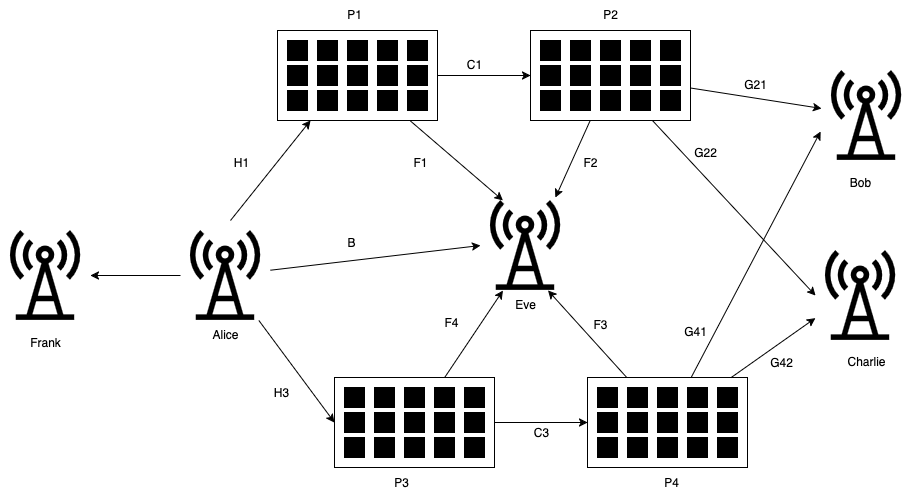
\includegraphics[width=\linewidth]{imgs/complex-situation.png}
  \caption{Complex setup for secure message transmission}
  \label{fig:correlation_sk2}
\end{figure}

More generally, we would have $M$ consecutive RIS (in series) that reflect a signal, $J$ legitimate receivers and $Q$ different paths of RIS (in parallel) to send the signal at the same time. \footnote{The paths could have a different number of RIS (for example, a path of three and another of two). The results would still hold.}

We will show simulation results for different combinations of ($M, J$), both with a single and double path. In all scenarios, $K = 2, N = 16, \eta = 0.9$ will be the number of antennas for all actors, the number of reflecting surfaces and the reflection coefficients. We take these parameters to compare the results to the original paper \cite{9328149}.

The direct link and the eavesdropper will try to understand the message by following the equation \eqref{eq:direct_detection}, while the receivers will try to understand it by following the equation \eqref{eq:reflection_detection}.

\subsubsection{Single RIS reflection (M=1)}

\begin{figure}[H]
  \centering
  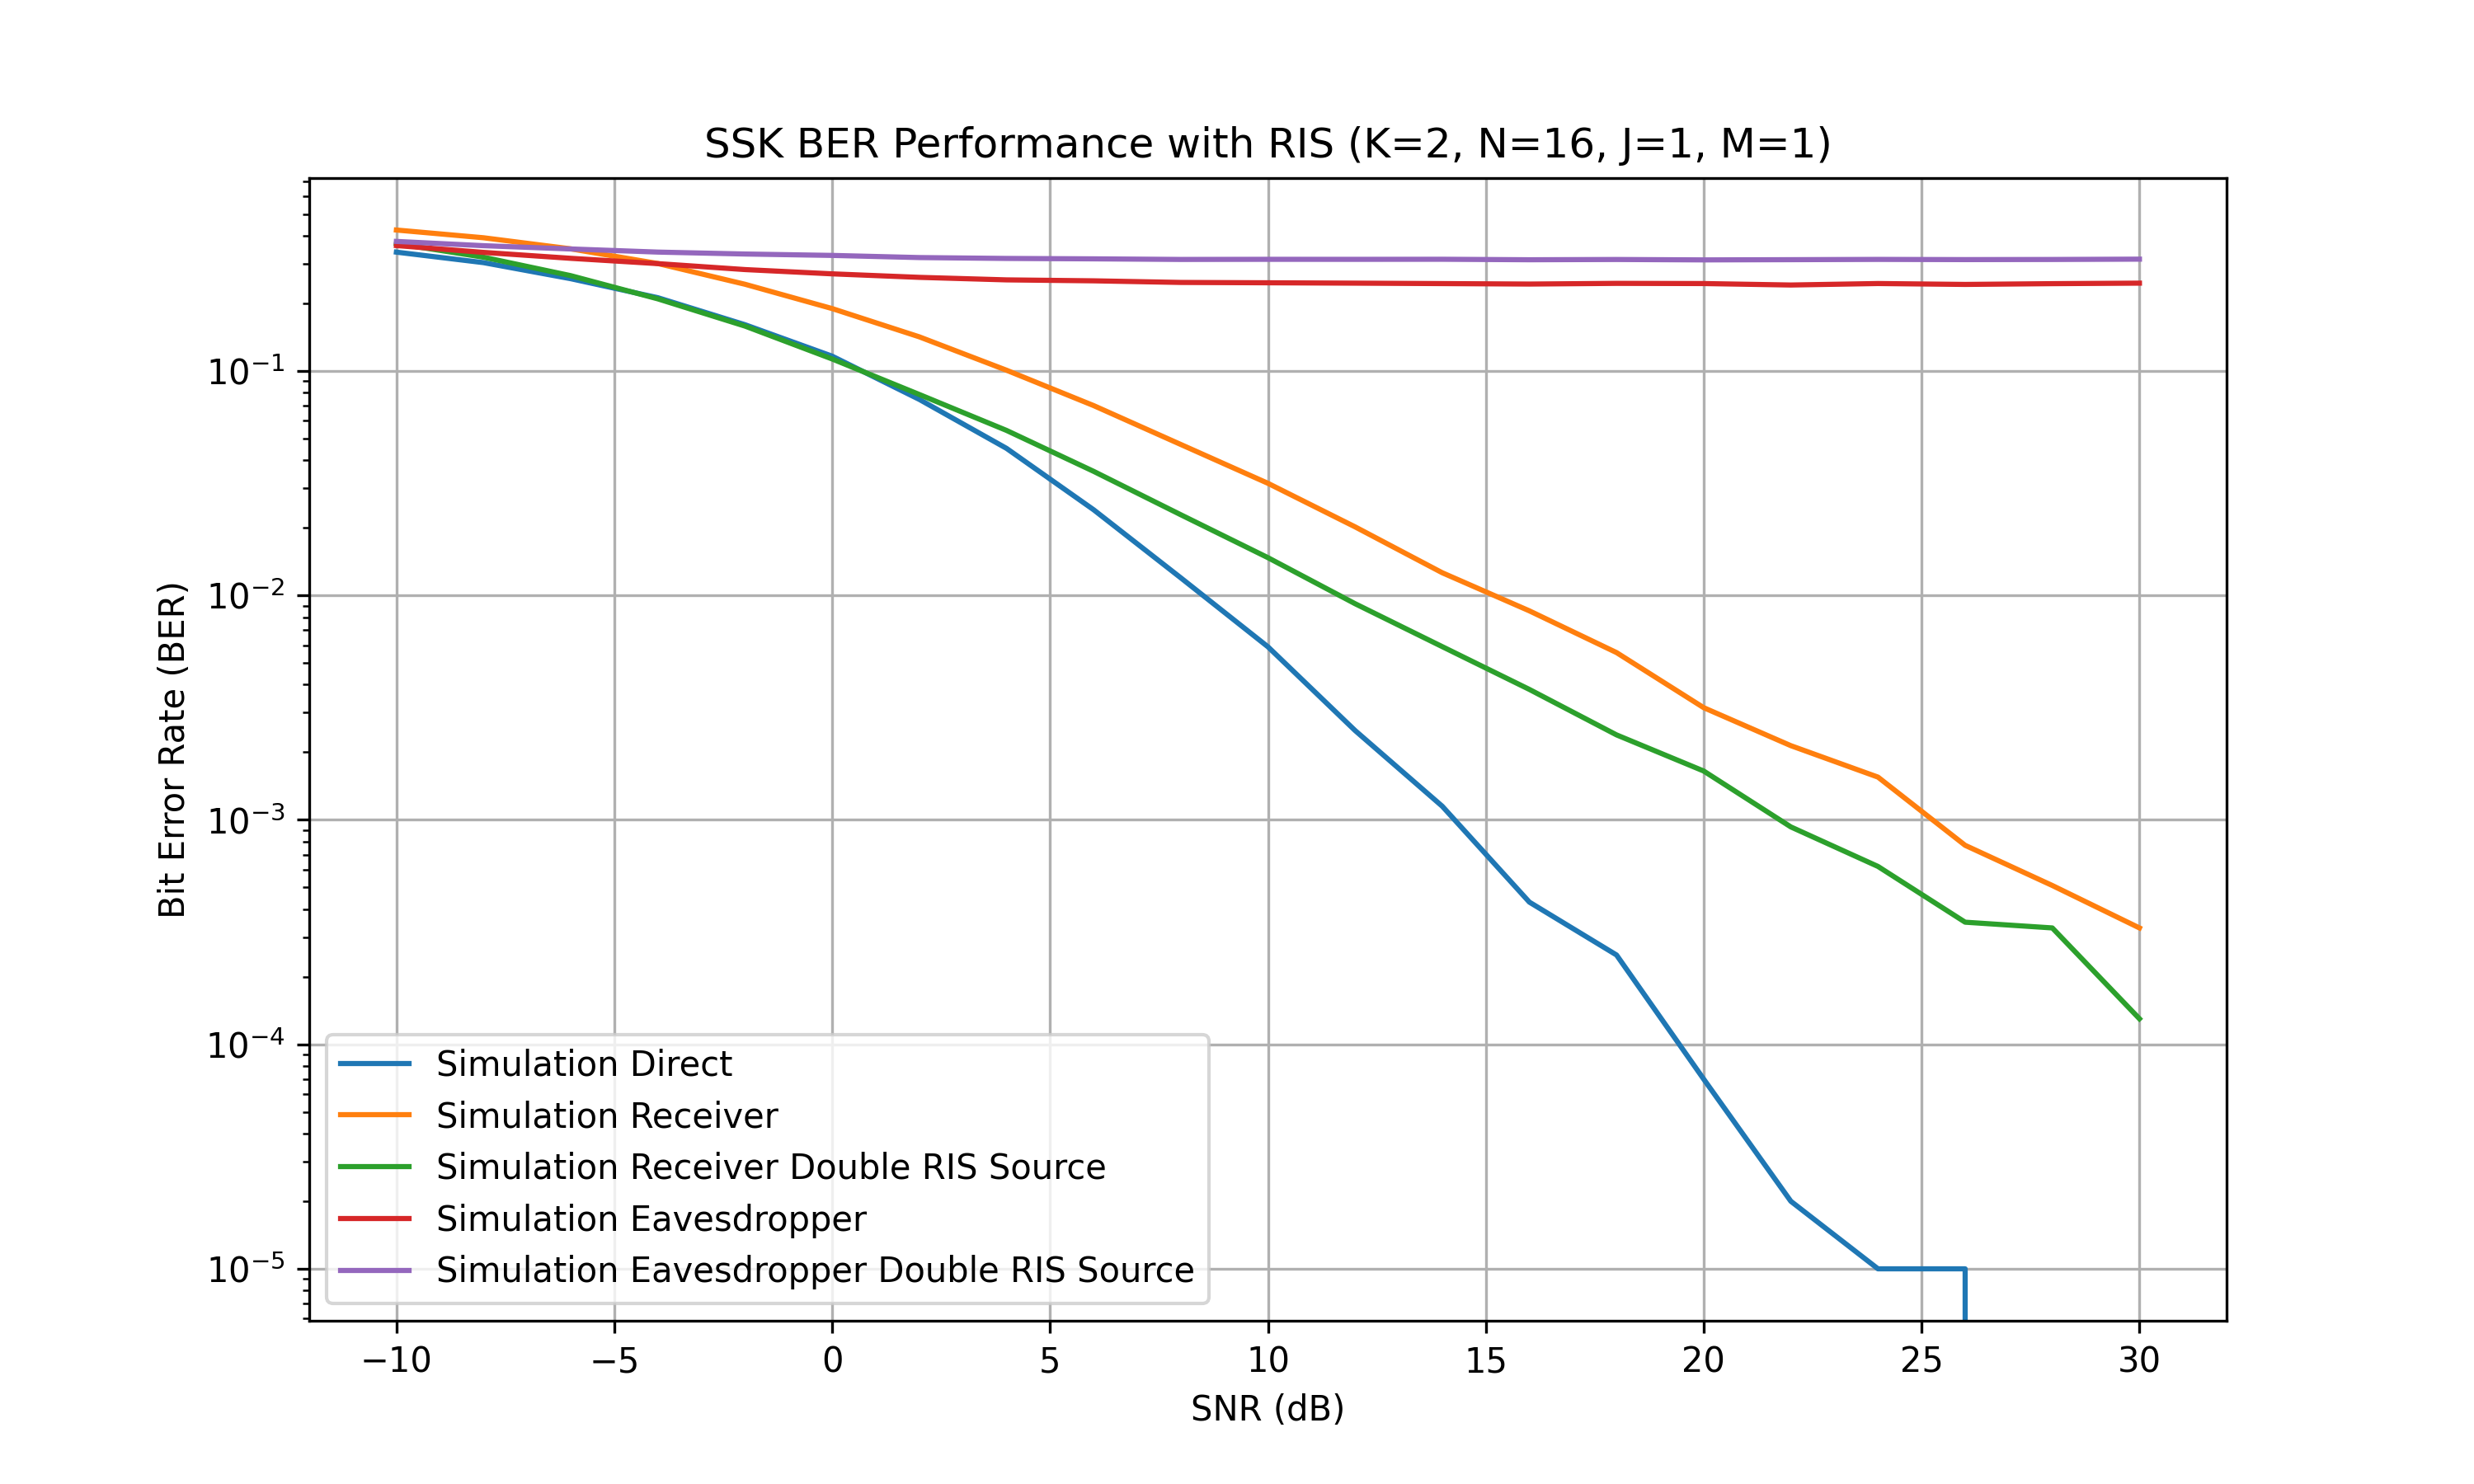
\includegraphics[width=0.9\linewidth]{imgs/ber-simulations/SSK BER Performance with RIS (K=2, N=16, J=1, M=1).png}
  \caption{SSK BER Performance with RIS (K=2, N=16, J=1, M=1)}
  \label{fig:simulation_j1_m1}
\end{figure}

We can see in ($M=1, J=1$) the results match with \cite{9328149}, for both \textit{Simulation Receiver} and \textit{Simulation Eavesdropper}.
\textit{Simulation Direct} is the strongest possible path, mainly because of the reflection loss due to $\eta$.
Combining two different RIS in parallel (\textit{Double RIS Source}) gives better signal to the receiver, while disturbing more the signal to the eavesdropper.

\begin{figure}[H]
  \centering
  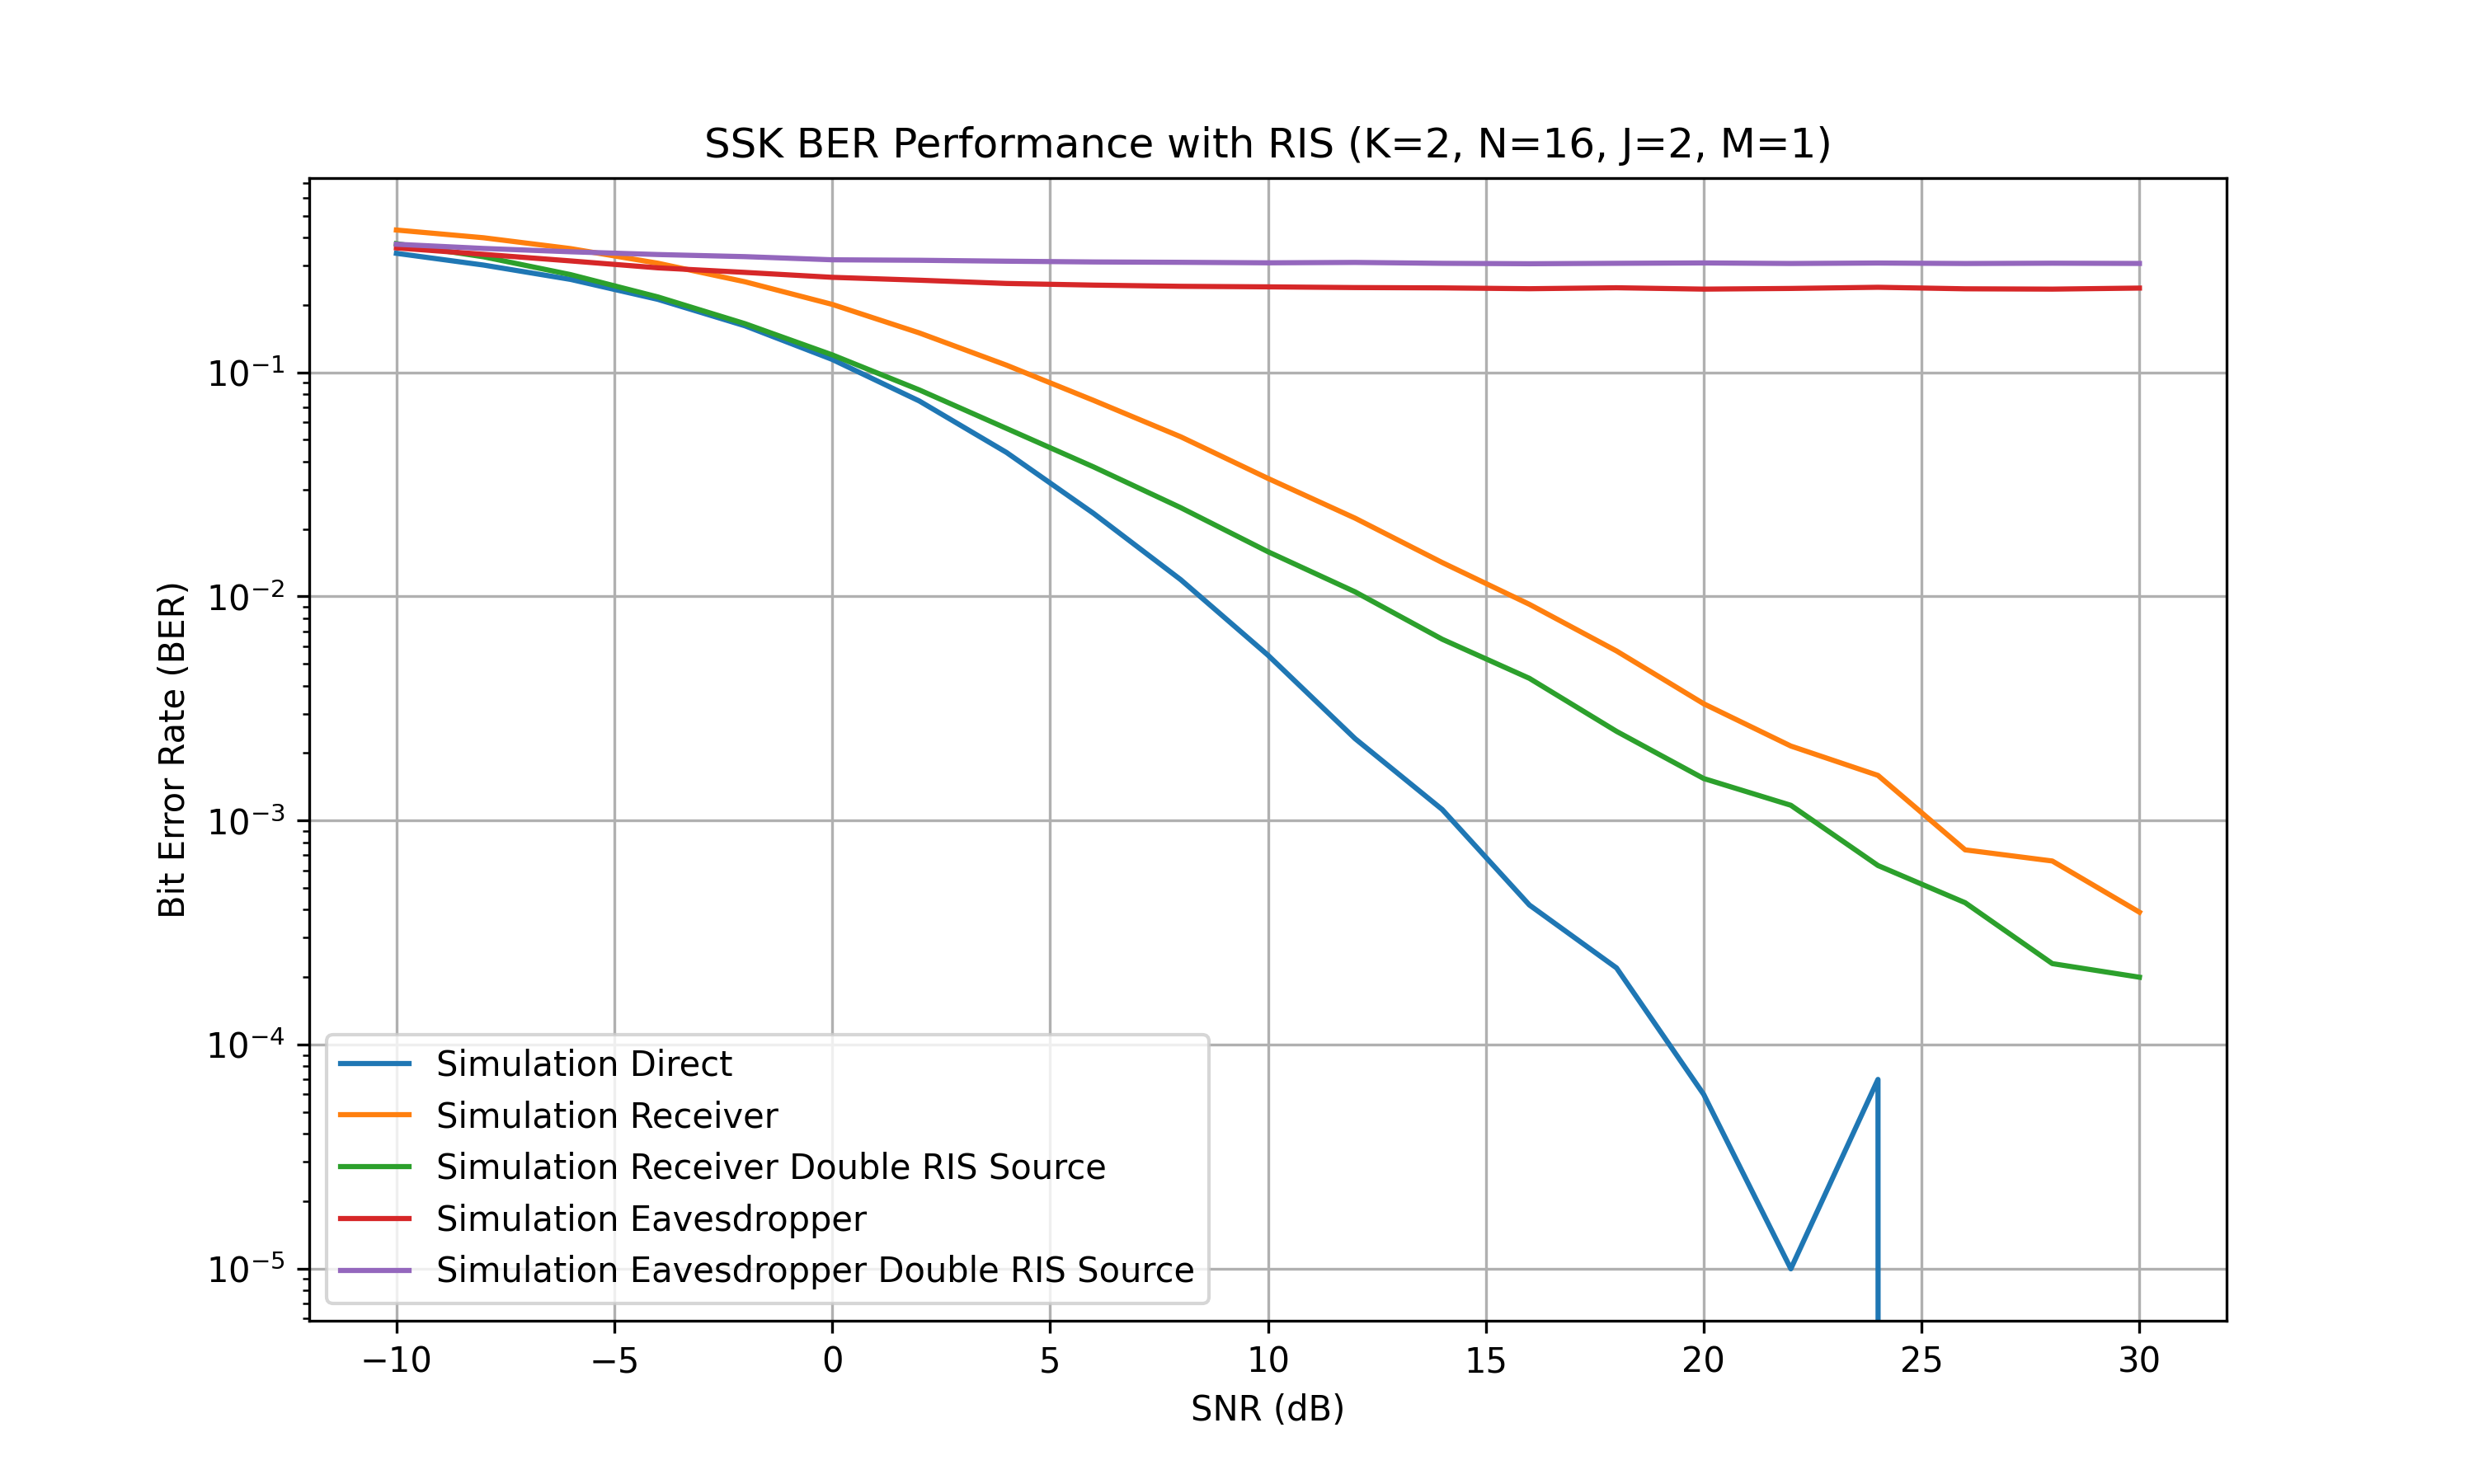
\includegraphics[width=0.9\linewidth]{imgs/ber-simulations/SSK BER Performance with RIS (K=2, N=16, J=2, M=1).png}
  \caption{SSK BER Performance with RIS (K=2, N=16, J=2, M=1)}
  \label{fig:simulation_j2_m1}
\end{figure}

Increasing the number of receivers does not influence the result of our framework: the receivers still get a good signal depending on the SNR, while the eavesdropper is not getting an advantage in understanding the message.

\subsubsection{Double RIS reflection (M=2)}

\begin{figure}[H]
  \centering
  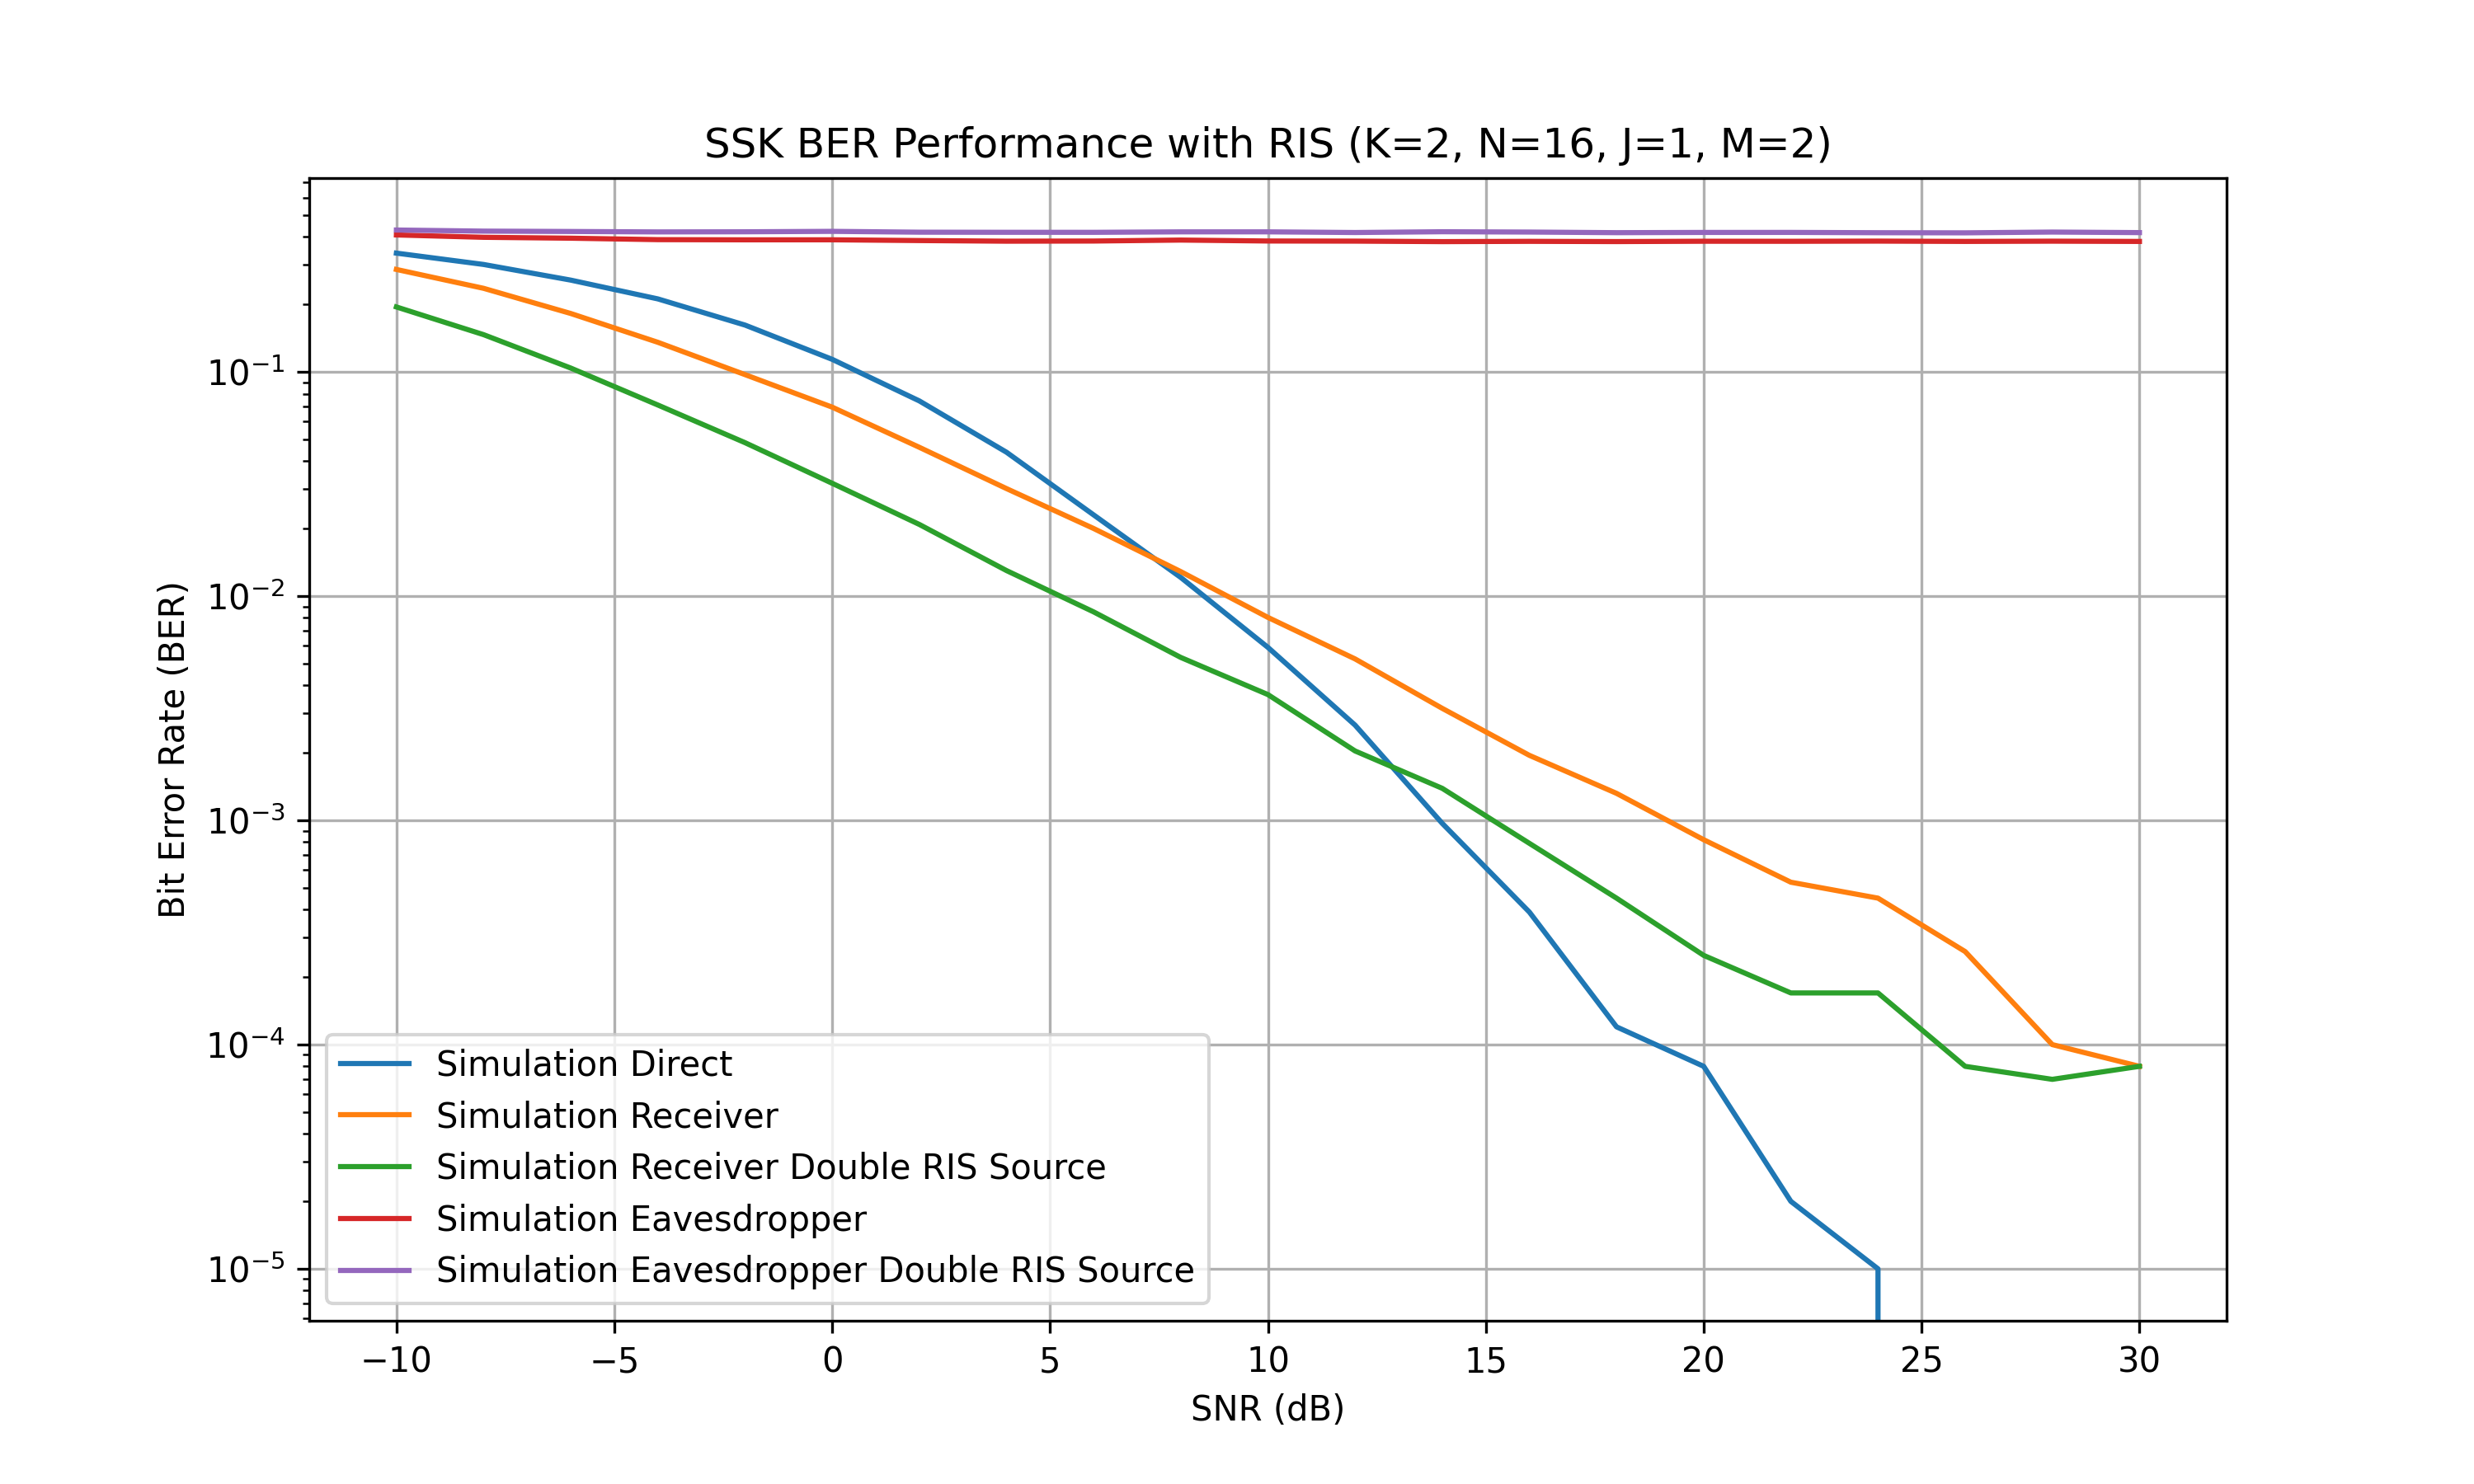
\includegraphics[width=0.9\linewidth]{imgs/ber-simulations/SSK BER Performance with RIS (K=2, N=16, J=1, M=2).png}
  \caption{SSK BER Performance with RIS (K=2, N=16, J=1, M=2)}
  \label{fig:simulation_j1_m2}
\end{figure}

With multiple RIS in series, the eavesdropper get a worse signal because of the double interference of the 2 RIS.
% \textbf{(TODO: Why the receiver is getting a better signal? Should it not be worse? Check normalization of the signal)}

\begin{figure}[H]
  \centering
  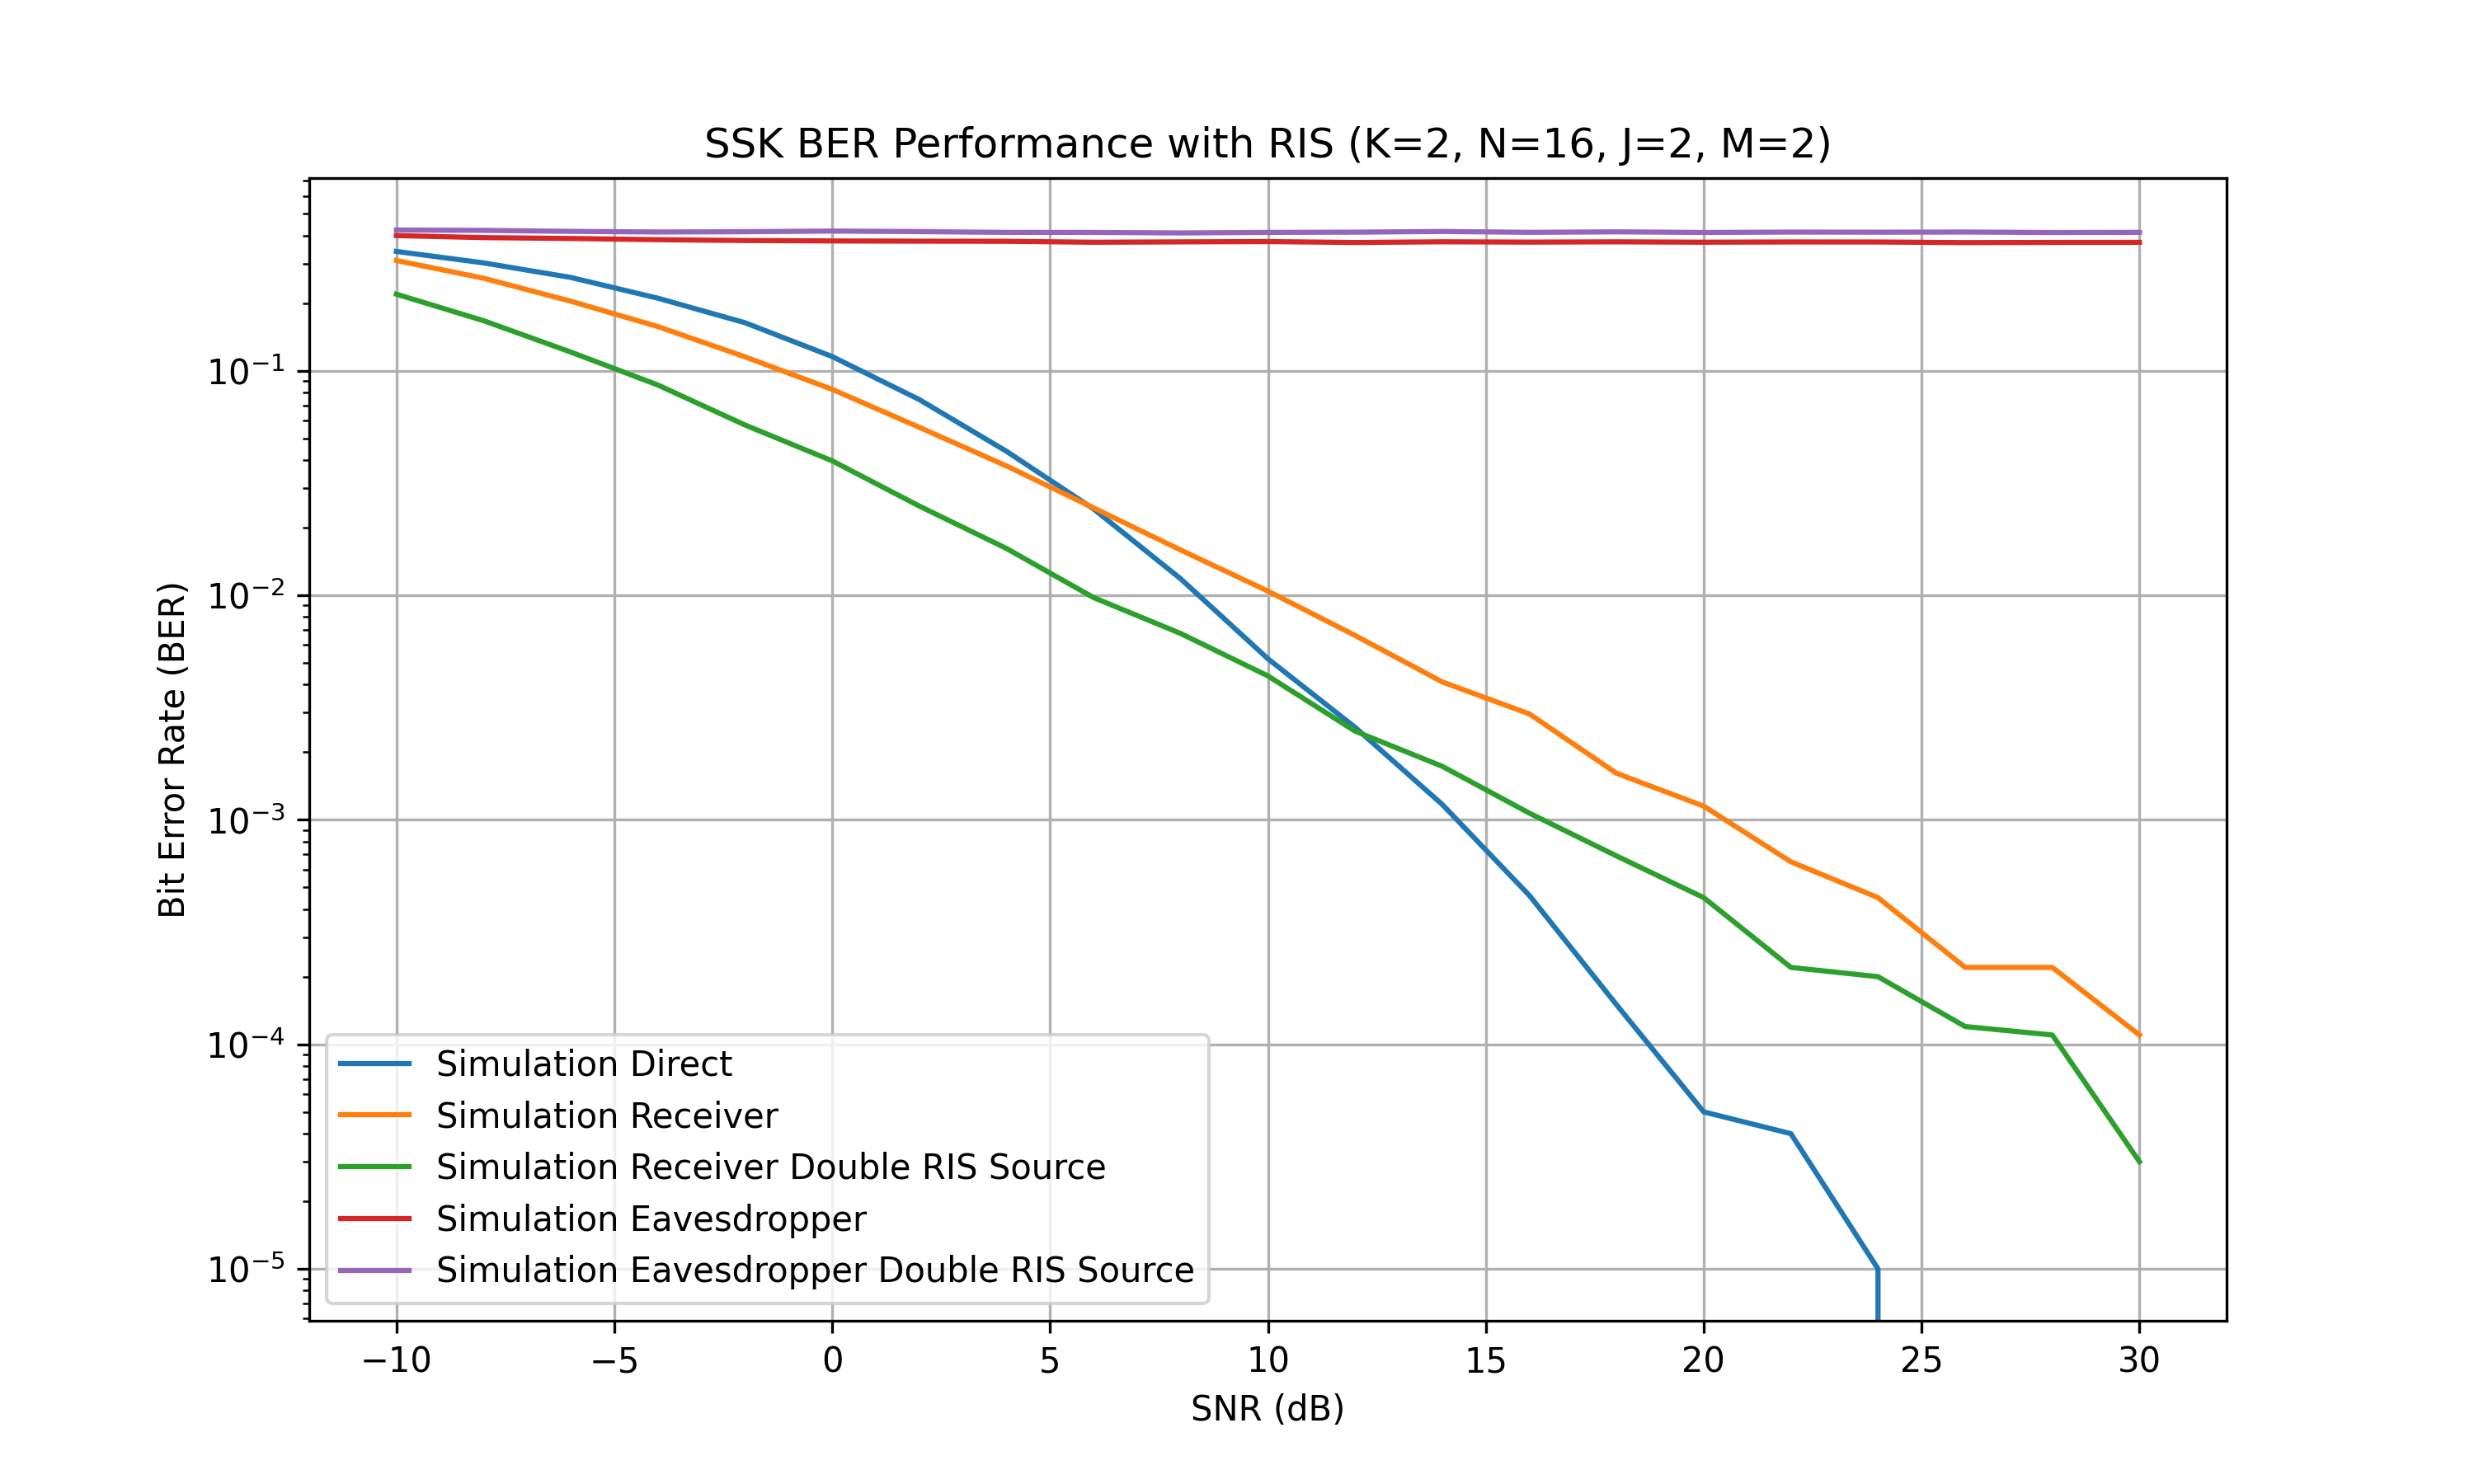
\includegraphics[width=0.9\linewidth]{imgs/ber-simulations/SSK BER Performance with RIS (K=2, N=16, J=2, M=2).png}
  \caption{SSK BER Performance with RIS (K=2, N=16, J=2, M=2)}
  \label{fig:simulation_j2_m2}
\end{figure}

Combining all together with two paths and double reflection to two receivers, our properties still hold strong.

\subsubsection{Theoretical conclusions}

From the graphs we can see that changes in the Signal to Noise Ratio (SNR) do not help the eavesdropper in understanding better the message. When there is a lot of noise, the performance is similar to the legitimate receivers, because no one is able to decipher the message.

When the noise level is much lower, and the signal strength much higher in comparison, the legitimate user understands the message much better, while the eavesdroppers do not. This is because even if the natural noise is reduced, the artificial noise caused by the unreadable RIS signal distorts the received communication for unwanted hearing users, and at the end the BER remains constant.

From \ref{fig:simulation_j1_m1}, we can already notice a lot of useful information. Firstly, the resulting graph comes out very similar to the one made by \cite{9328149}. This is good, because now we have confirmation of our base work, useful to also be confident about our extension and mathematical modifications. In their graph Fig 5.a, they show different lines based on multiple reflection coefficients $\eta$, while we used only $\eta = 0.9$, and different Rician Factors to model the power difference between the direct signal and the reflected one, while we used only the eavesdropper with value equal to $1$. Comparing those two particular lines to ours "Simulation Receiver" and "Simulation Eavesdropper".

We can focus better on our additions. Firstly, by adding the raw performance of the direct link, we can see that our reflected signal still gives for our legitimate users a solid link to communicate, that offers great performance even when considering the reflection coefficient loss $\eta$. Second, we can see that by adding a second reflection path with a double RIS source, our users get better signal while eavesdroppers get even more noise.

In the next graph \ref{fig:simulation_j2_m1} we can see how adding a second legitimate user does not influence the performance of our proposed general solution. This is great: our solution is more scalable, with the same capability to serve data securely. Adding more user constraints does not make our system more vulnerable or less understandable.

In \ref{fig:simulation_j1_m2} and \ref{fig:simulation_j2_m2} we can make similar considerations. Even by adding more reflections for each single path, our framework still shows high promises. We can see, however, that the legitimate receivers BER falls much faster. This is because without considering signal strength reductions due to path loss, multiplying the related matrices improves the overall signal calculated. This is why we also added a new type of simulation to our research, to test our framework with more realistic and specific scenarios.

\newpage
\subsection{BER realistic scenario simulation}

In this section, we evaluate our framework in more realistic spatial environments by creating BER heatmaps that show security performance across different physical locations. We model various path loss scenarios and analyze how they affect the security properties of our system.

We model the channel gain $H$ and the path loss based on the distance between the actors. We will define $\lambda$ as the wavelength of the signal, and $d$ as the distance between two actors.

\subsubsection{Channel gain calculation}

We model the Rician fading \cite{Rician_fading} matrix $\bm{\Xi}$, to consider possible fading due to multipath interference. Using the Shape Parameter $\tau$, defined as the ratio of the power contributions by line-of-sight path to the remaining multipaths, and the Scale parameter $\xi$, defined as the total power received in all paths, we can calculate

\begin{equation}
  \nu^2 = \frac{\tau \xi}{1 + \tau}
\end{equation}
\begin{equation}
  \sigma^2 = \frac{\xi}{2(1 + \tau)}
\end{equation}

and we can generate $\bm{\Xi}$ by creating a random complex matrix where the real and the imaginary values are extracted from a gaussian distribution $C(\frac{\nu}{\sqrt{2}}, \sigma)$ \cite{Rice_distribution}

Then, given an actor $r$ with $n_r$ antennas disposed as a \textit{uniform linear array}, we can define the \textit{unit spatial signature in the directional cosine $\Omega = cos \phi$} \cite{Fundamentals_Wireless_Communication_chapter7} as

\begin{equation}
  e_r(\Omega) = \frac{1}{\sqrt{n_r}}
  \begin{bmatrix}
    1                                \\
    exp(-j2\pi\Delta\Omega)          \\
    exp(-j2\pi2\Delta\Omega)         \\
    \vdots                           \\
    exp(-j2\pi(n_r - 1)\Delta\Omega) \\
  \end{bmatrix}
\end{equation}

where
\begin{itemize}
  \item $\Delta$ is the distance between the antennas (usually $\lambda / 2$)
  \item $\phi$ is the angle of incidence of the line-of-sight onto the actor antenna
\end{itemize}

and we can model the channel gain matrix \cite{Fundamentals_Wireless_Communication_chapter7} as

\begin{equation}
  \bm{H} = \bm{\Xi} \odot \sqrt{n_t n_r} exp(-j2 \pi d / \lambda) e_r(\Omega_r) e_t(\Omega_t)^H
\end{equation}

We will use this equation both for a direct transmission between two actors, or between an actor and a RIS.

\subsubsection{Path loss calculation}

We begin by modeling the free space path loss \cite{Free_space_path_loss} between two points as
\begin{equation}
  \bm{PL} = ((4 \pi / \lambda)^2 d^k)^{-\frac{1}{2}}
\end{equation}
where $k$ is equal to $2$ when the antennas are isotropic, meaning they radiate power uniformly in all directions in three dimensional space. We will use $k = 2$ for our simulations, even if it is only a theoretical concept.

For a direct LOS communication between the transmitter and another actor (either a legitimate receiver or an eavesdropper), the signal received from input $x$ would be

\begin{equation}
  y = \bm{PL}_B * \bm{B}x
\end{equation}

Given a reflected signal with channel gain $GPH$, where
\begin{itemize}
  \item $\bm{G}$ is the communication transmitter-RIS
  \item $\bm{H}$ is the communication RIS-actors
  \item $\bm{P}$ is the RIS reflection coefficient diagonal matrix
\end{itemize}
we have two different LOS communications. We have different ways of calculating the total path loss:
\begin{itemize}
  \item we consider the RISs to be active, meaning they amplify the signal received before reflecting it and so they negate the path loss reduction. The signal received would be $y = PL_H * GPHx$. As a result, in case of multiple RISs, only the last connection path loss is considered. We will call this as a \textit{active path loss}
  \item we consider two separate path losses, one for each LOS. The signal received would be $y = PL_G * PL_H * \bm{GPH}x$. In case of multiple RISs, we multiply the path loss of all connections. We will call this as a \textit{product path loss}. This usually represents a non directional, isotropic RIS, where the reflected signal is scattered uniformly across all directions and the path loss is significant.
  \item we consider one single path loss from the sum of the two distances ($d = d_{t-RIS} + d_{RIS-r}$). The signal received would be $y = PL_{G+H} * \bm{GPH}x$. In case of multiple RISs, we add all the distances. We will call this as a \textit{sum path loss}. This is a simplification of a much more complex type of RIS, called directional RIS, which modulates the phase and magnitude of its elements to redirect the signal in a single direction. This regulation reduces the path loss caused by the second reflection, in relation to the number of elements $N$ of the RIS. It is possible to read more in the paper \cite{8888223}. It is important to note that, while we are showing results of how a scenario with this type of path loss may act, we will just vary the calculation of the path loss for each point in the map, and will not make any calculations of directional phases themselves. The RIS would still look like an uniform sending relay, and it is included in the document to show the potentiality of our framework in that condition. So for the \textit{sum path loss}, it is important to remember this theoretical limitation. For example, we will show the BER for two different receivers in different locations and various situations, but of course it not be possible to serve in multiple direction for that type of RIS. Mathematically, you could see our graphs of this kind as showing the situation where we have  $\lim_{X \to \infty} X$ RIS, all in the same position, each one directed to a different point of the map, with none interfering with each other. It is most certainly an interesting topic for a later research, the actual implementation of our framework with the constraint of directionality of the RIS. This could be done by putting more constraints on the vector $q$ in \eqref{q_random_vector}.
\end{itemize}

We will show the main graph, showing the heatmap of the BER for each square, and two or three graphs, showing the logarithmic heatmap of the power received in that point from the transmitter of from a reflection passing through a RIS. For the BER, you could consider all spots not signed by a label as a possible eavesdropper location. \textbf{T} represents the transmitter, \textbf{P*} are the RIS and \textbf{R*} the legitimate receivers.

\subsubsection{Single angle of reflection, aided by 1 RIS}

Here we have a standard scenario where the transmitter has only a conical view between two buildings, and the receivers do not have direct LOS. What we want to show is that without LOS the message is completely unreadable except for the legitimate users, while the spots in LOS with the transmitter still receive various levels of noise.

For all of the three kinds of path loss, we will have the following parameters: $\lambda = 0.08m$, as standard for 5G connections, $ \tau = 0.6, \xi = 1, \eta = 0.9, SNR = 10db, K = 4, N = 25$. In particular, we want to use for this scenario a higher number of antennas per actor and reflecting elements per RIS to show: 1) a bit more complex configuration that the standard $K = 2, N = 16$; 2) show that the BER does have an upper limit on 0.5, the value of random guessing. This is because, even if a higher $K$ could make one suppose you have only $1/K$ probability of guessing the turned on antenna, the actual bit representation is only made of $0$ and $1$, and thus the probability of error for each bit is $0.5$.

\paragraph*{Path loss: active}

We can see here how this type of path loss ensures that in the vicinity of the RIS the Bit Error Rate remains very high, thanks to the active power component of the RIS itself.

We can see the reflected signal from the RIS has the RIS itself as the center.

\begin{figure}[H]
  \centering
  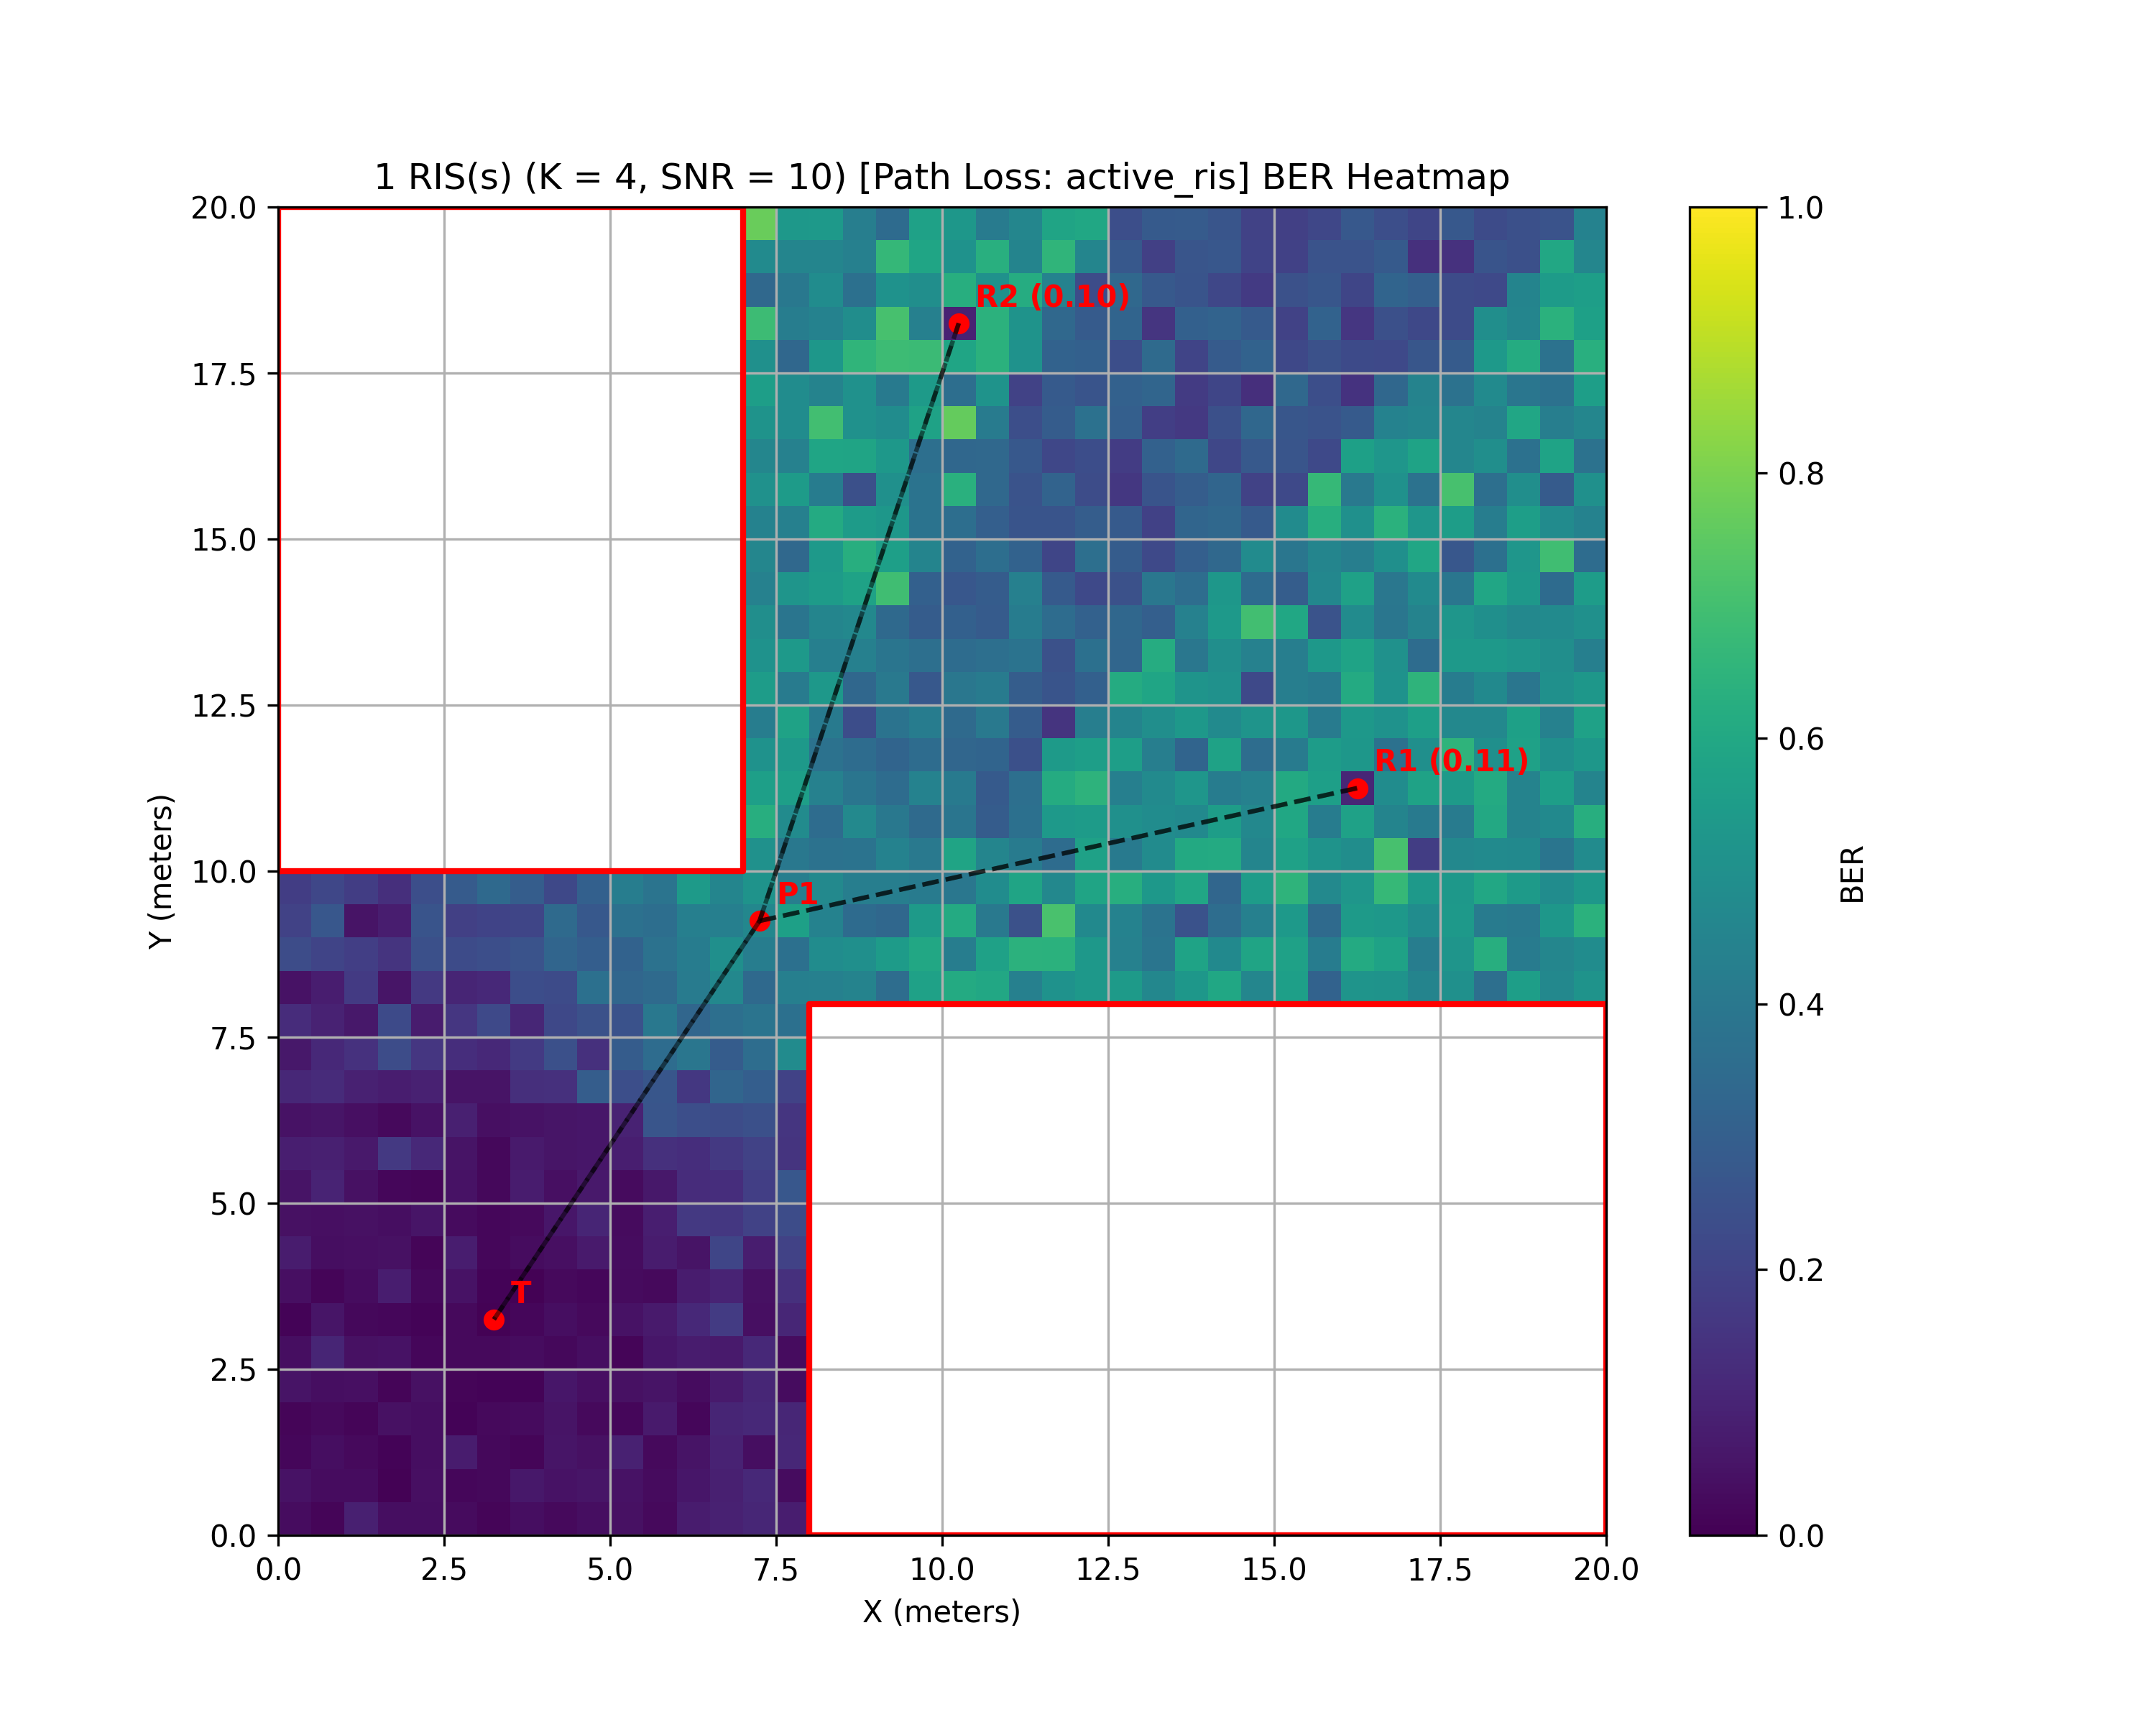
\includegraphics[width=0.7\linewidth]{imgs/heatmap-simulations/1 RIS(s) (K = 4, SNR = 10) [Path Loss_ active_ris] BER Heatmap.png}
  \caption{1 RIS(s) [Path Loss: active ris] BER Heatmap}
\end{figure}

\begin{figure}[H]
  \centering
  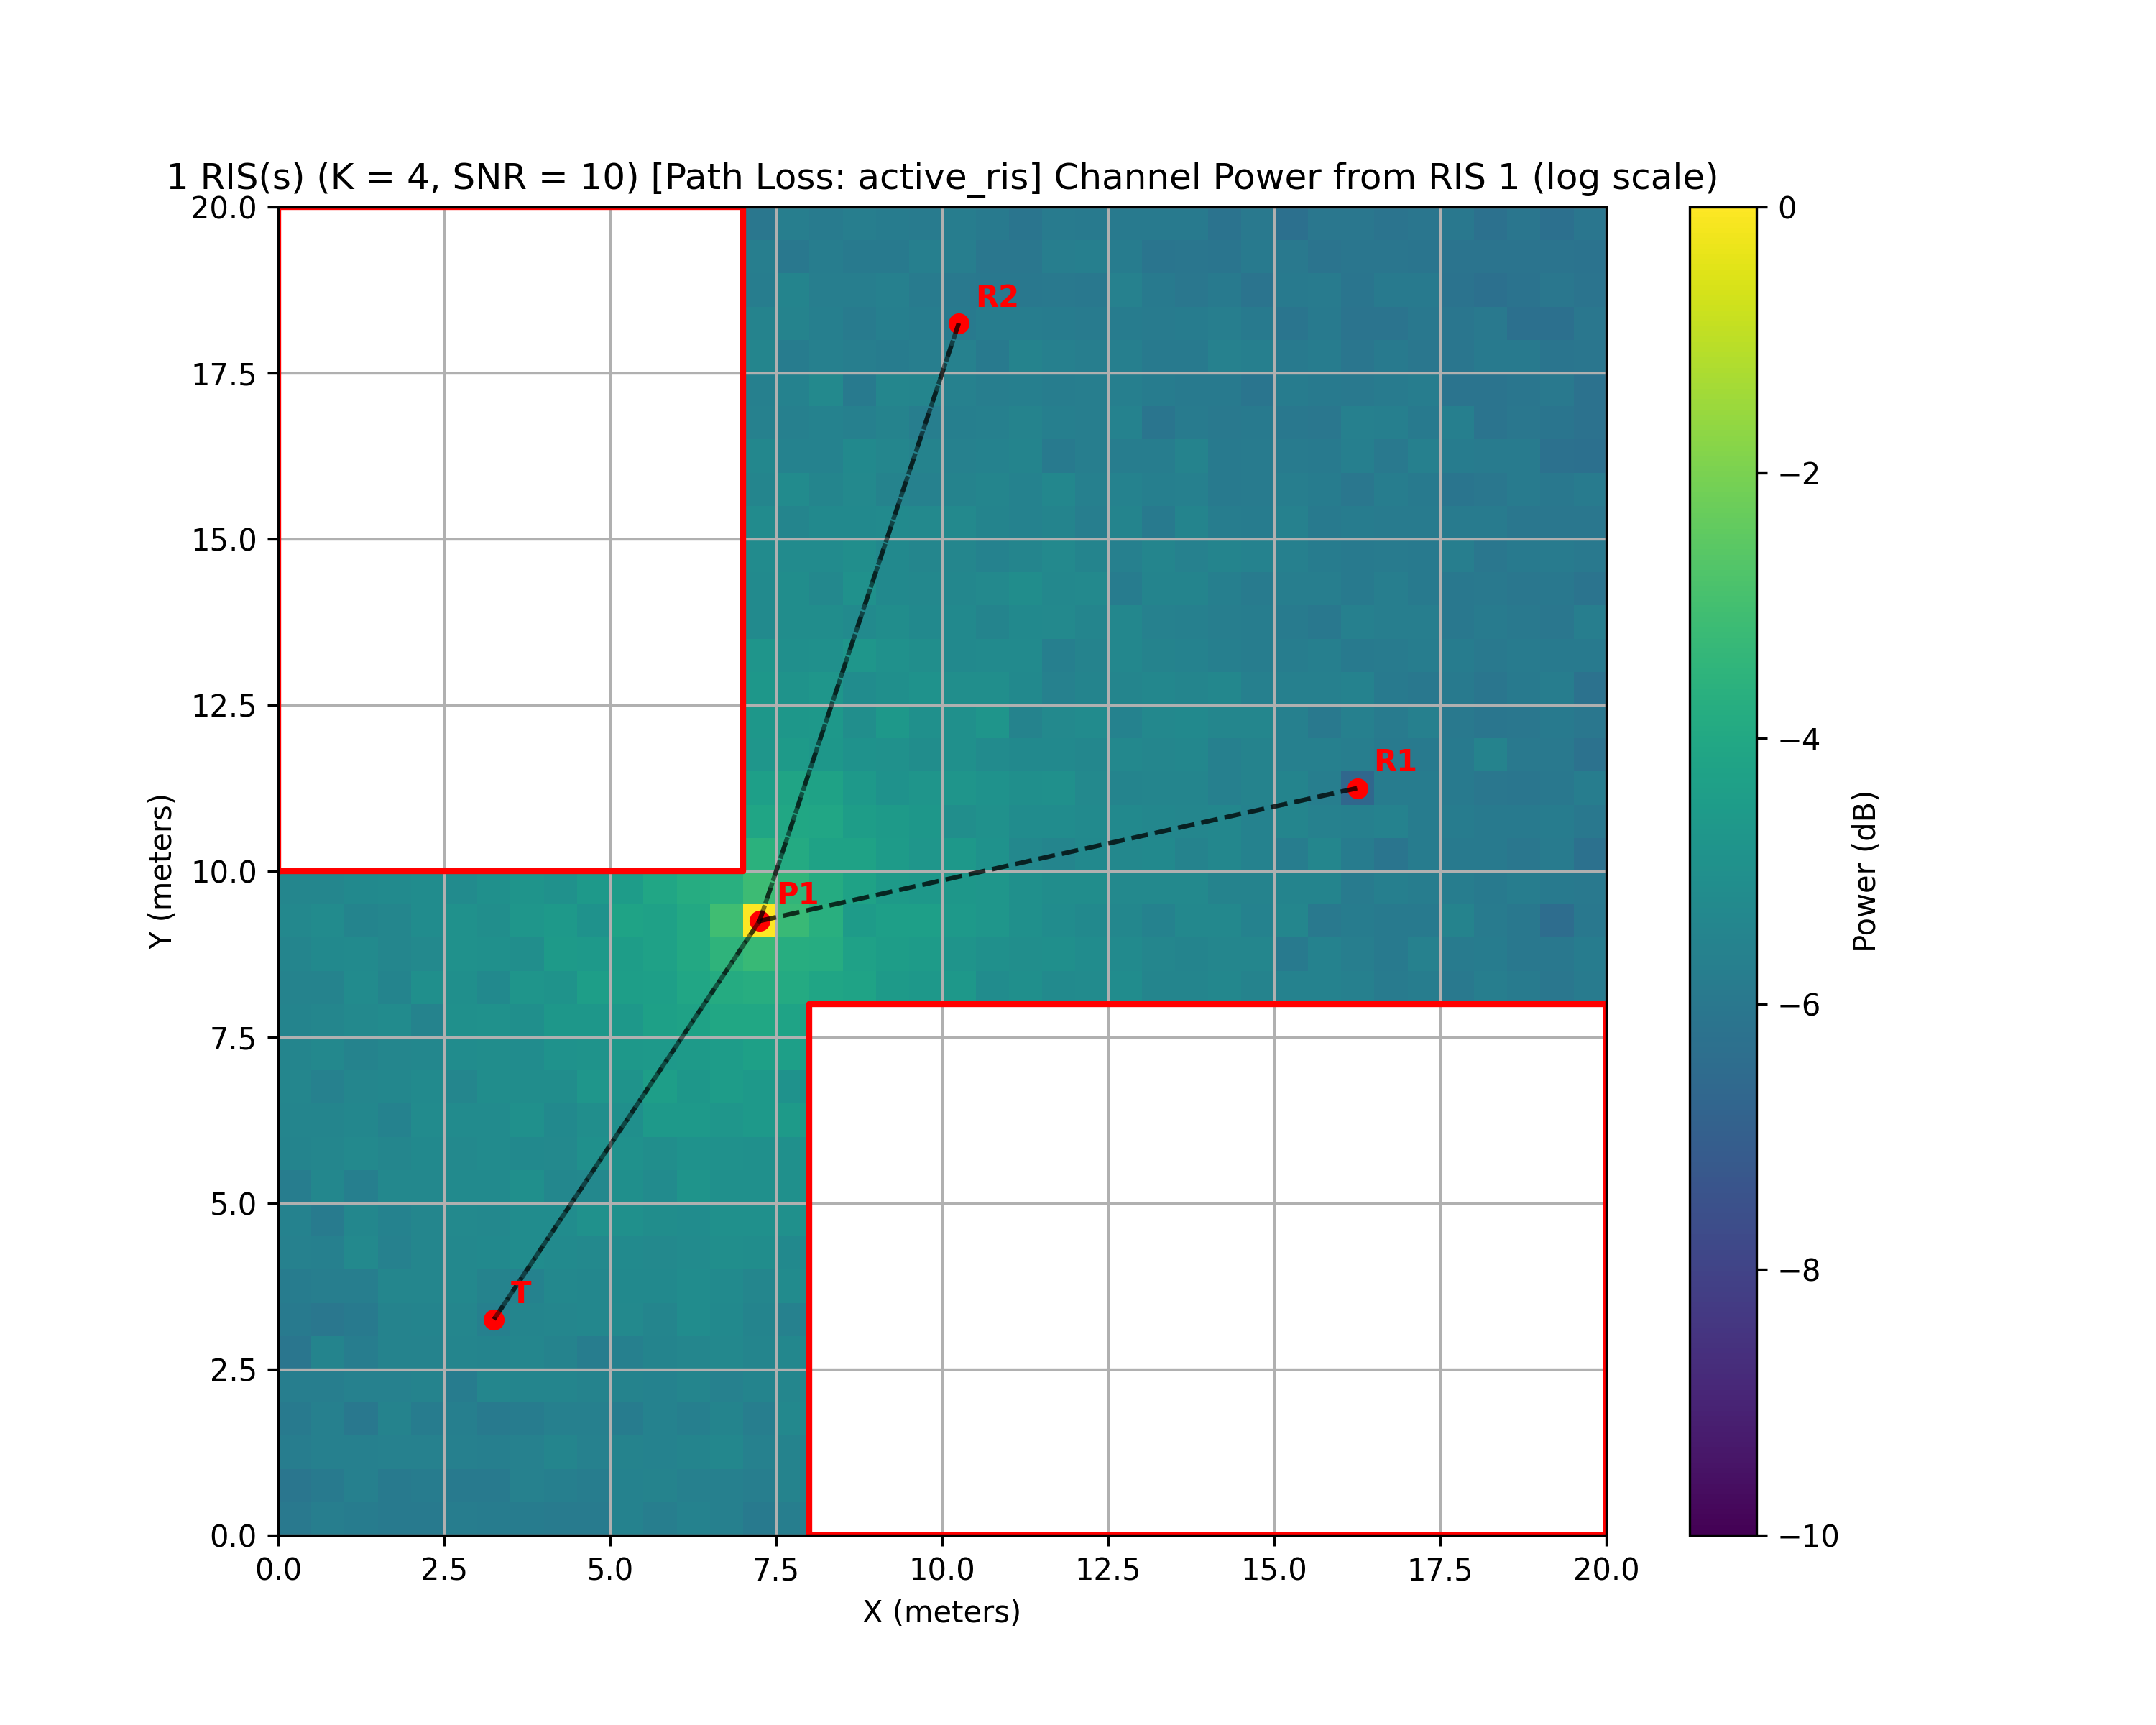
\includegraphics[width=0.7\linewidth]{imgs/heatmap-simulations/1 RIS(s) (K = 4, SNR = 10) [Path Loss_ active_ris] Channel Power from RIS 1 (log scale).png}
  \caption{1 RIS(s) [Path Loss: active ris] Channel Power from RIS 1 (log scale)}
\end{figure}

\begin{figure}[H]
  \centering
  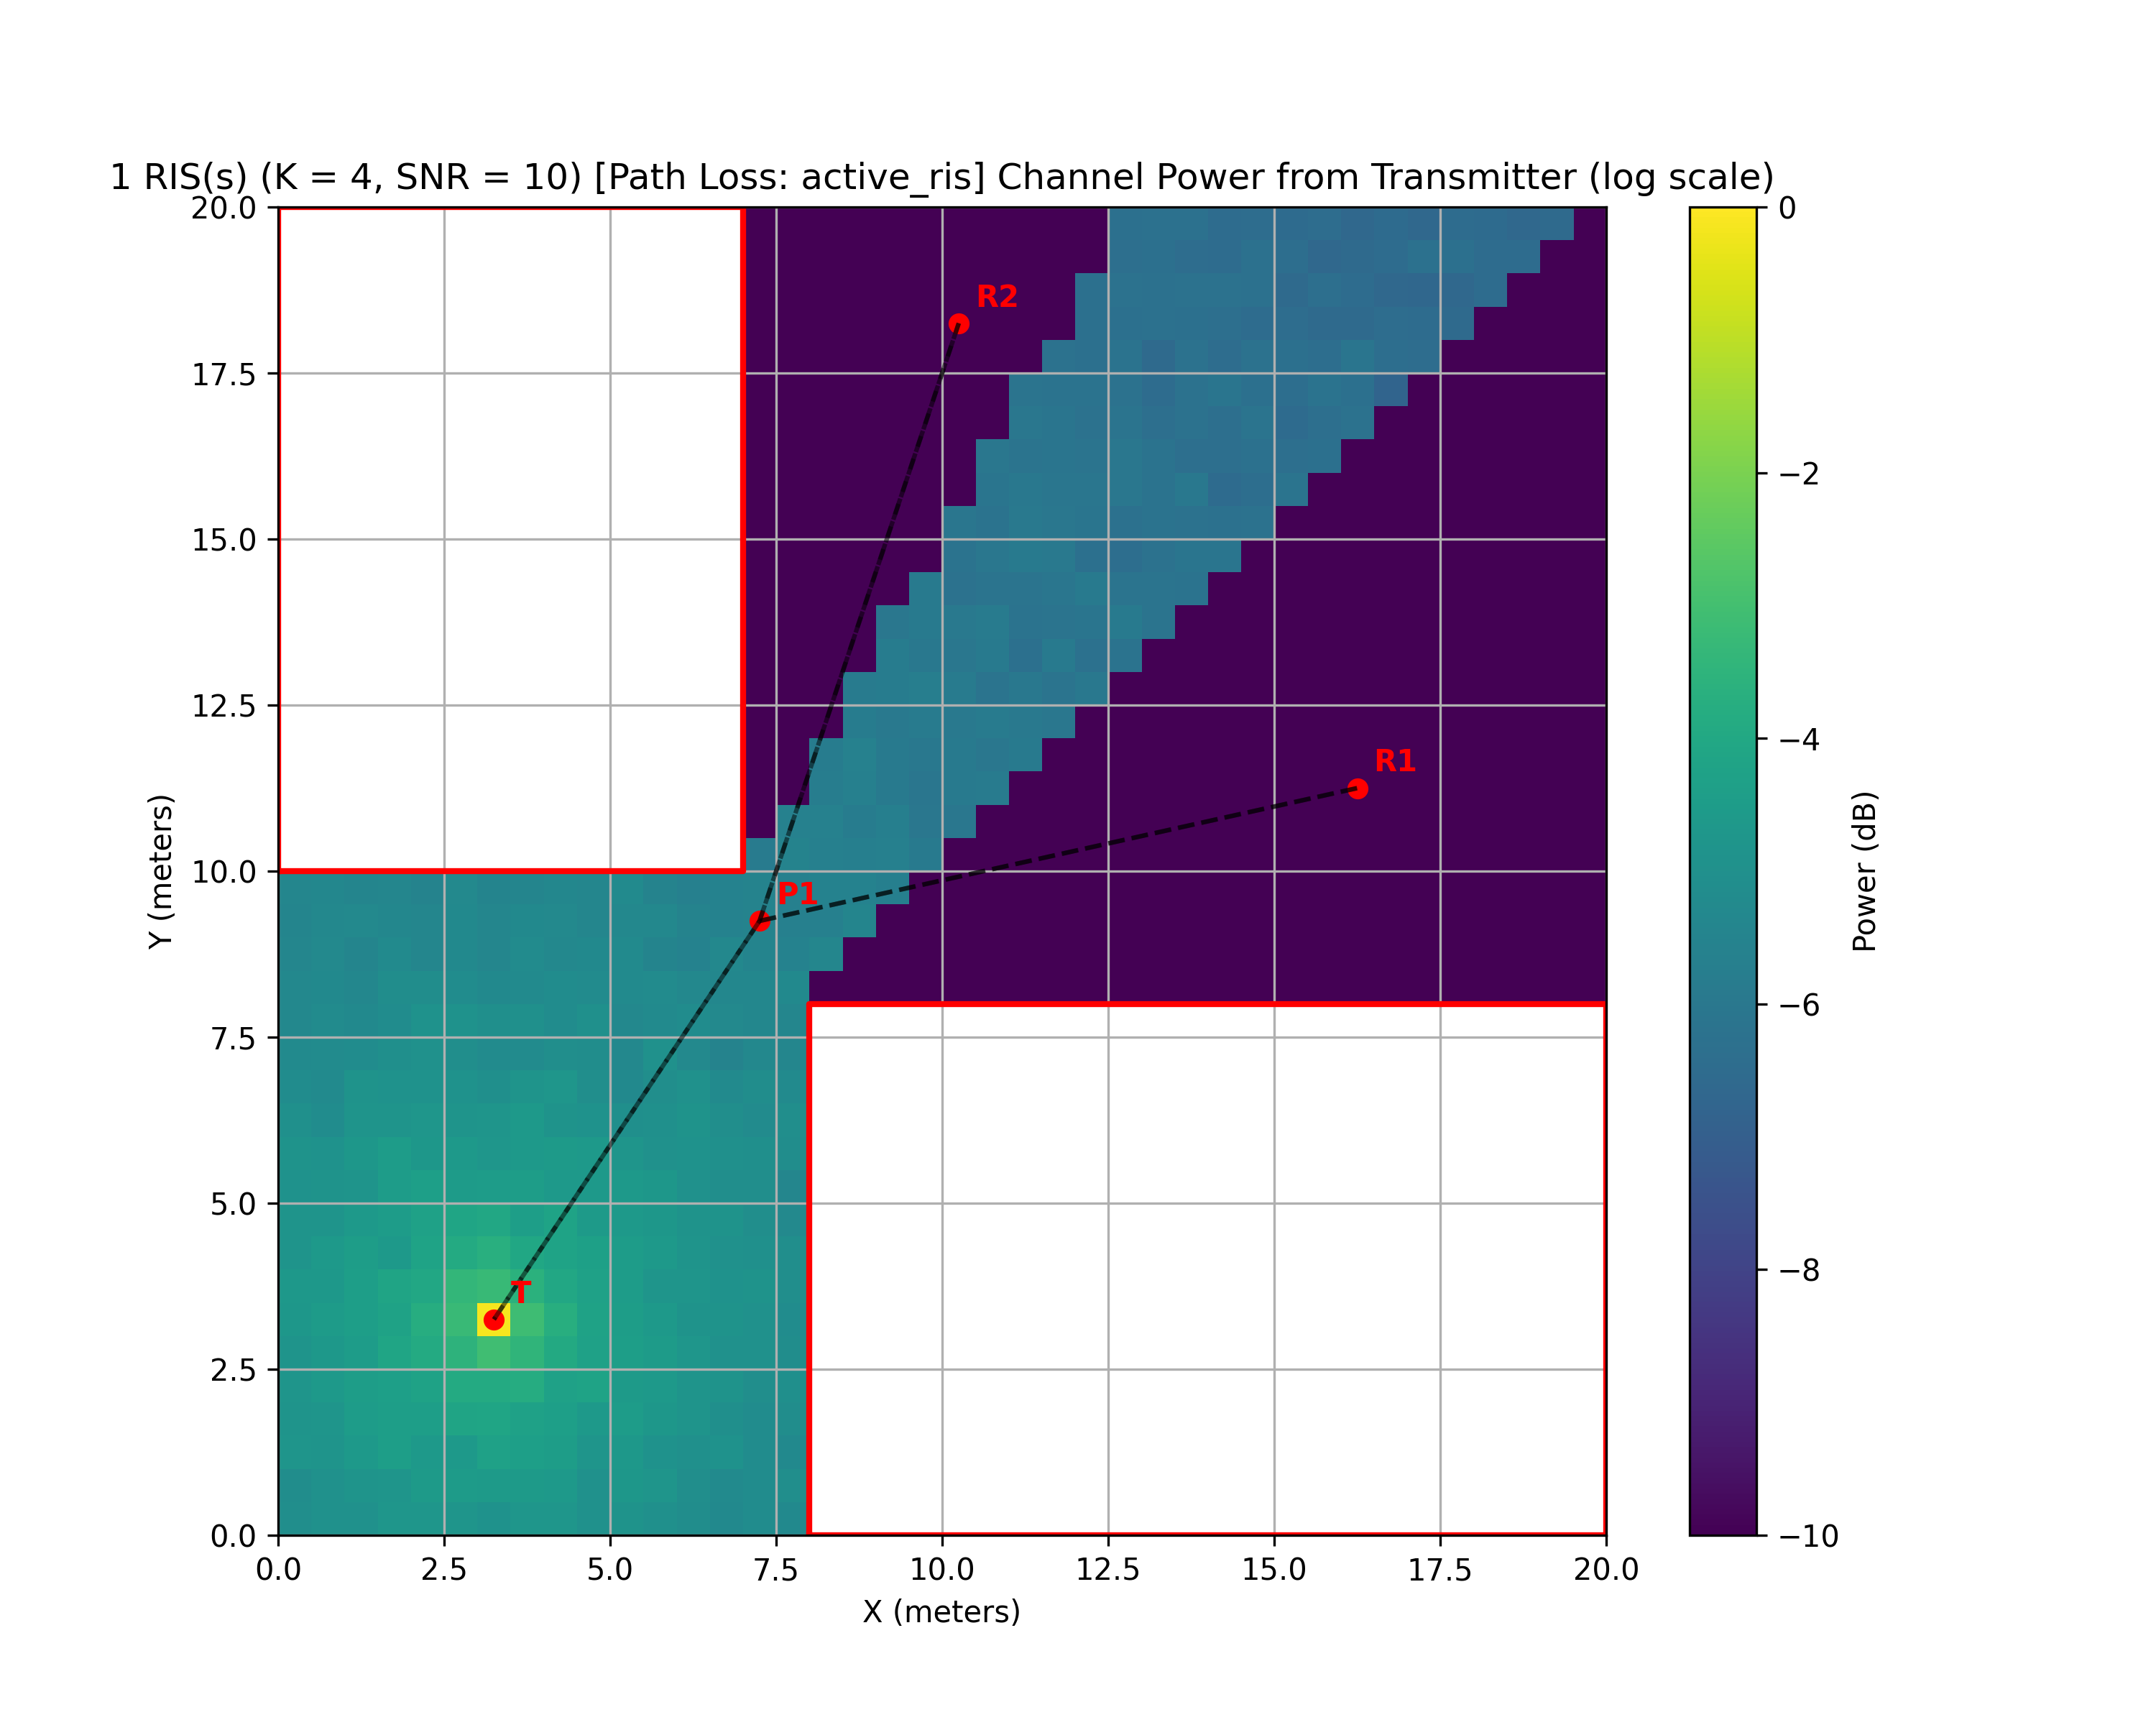
\includegraphics[width=0.7\linewidth]{imgs/heatmap-simulations/1 RIS(s) (K = 4, SNR = 10) [Path Loss_ active_ris] Channel Power from Transmitter (log scale).png}
  \caption{1 RIS(s) [Path Loss: active ris] Channel Power from Transmitter (log scale)}
\end{figure}

\paragraph*{Path loss: product}

With this type of path loss, the signal coming from the RIS has significantly less power than the direct link from the transmitter, and cannot influence significantly the outcome. Outside LOS, the framework still works as expected.

The power of the signal reflected from the RIS is so low, it does not show in the heatmap, as it is lower than $1e-10$.

\begin{figure}[H]
  \centering
  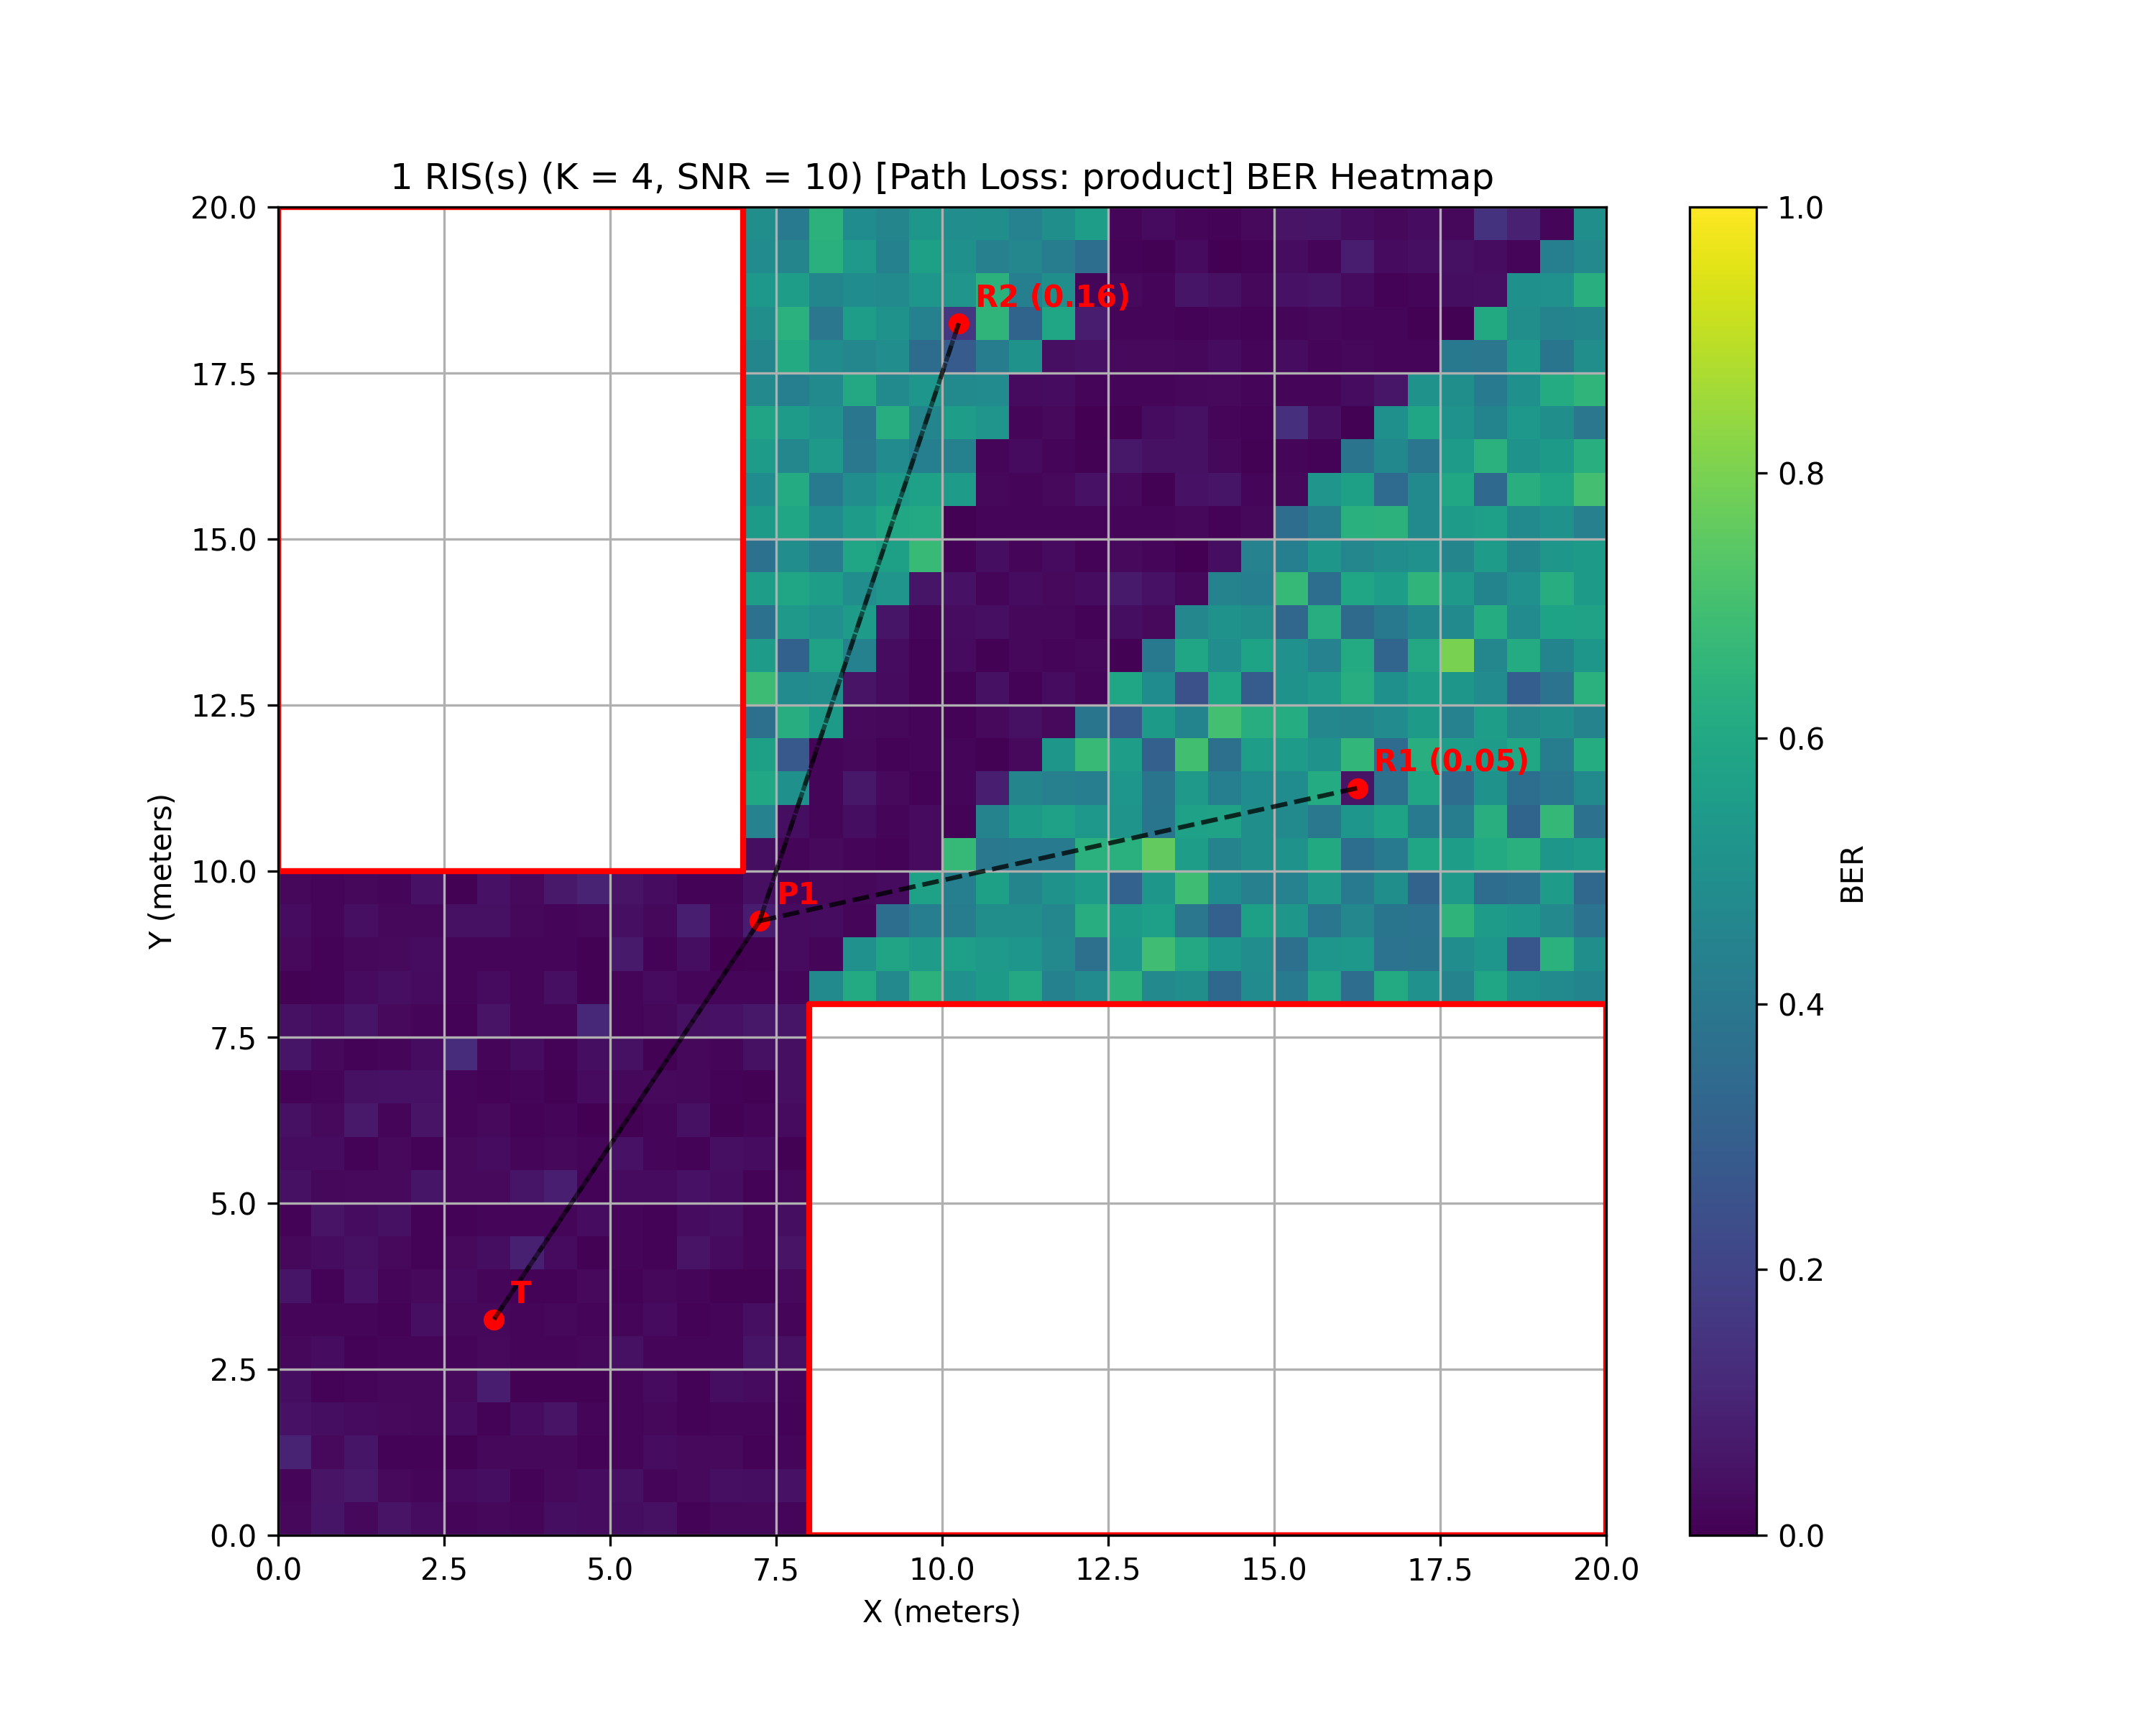
\includegraphics[width=0.7\linewidth]{imgs/heatmap-simulations/1 RIS(s) (K = 4, SNR = 10) [Path Loss_ product] BER Heatmap.png}
  \caption{1 RIS(s) [Path Loss: product] BER Heatmap}
\end{figure}

\begin{figure}[H]
  \centering
  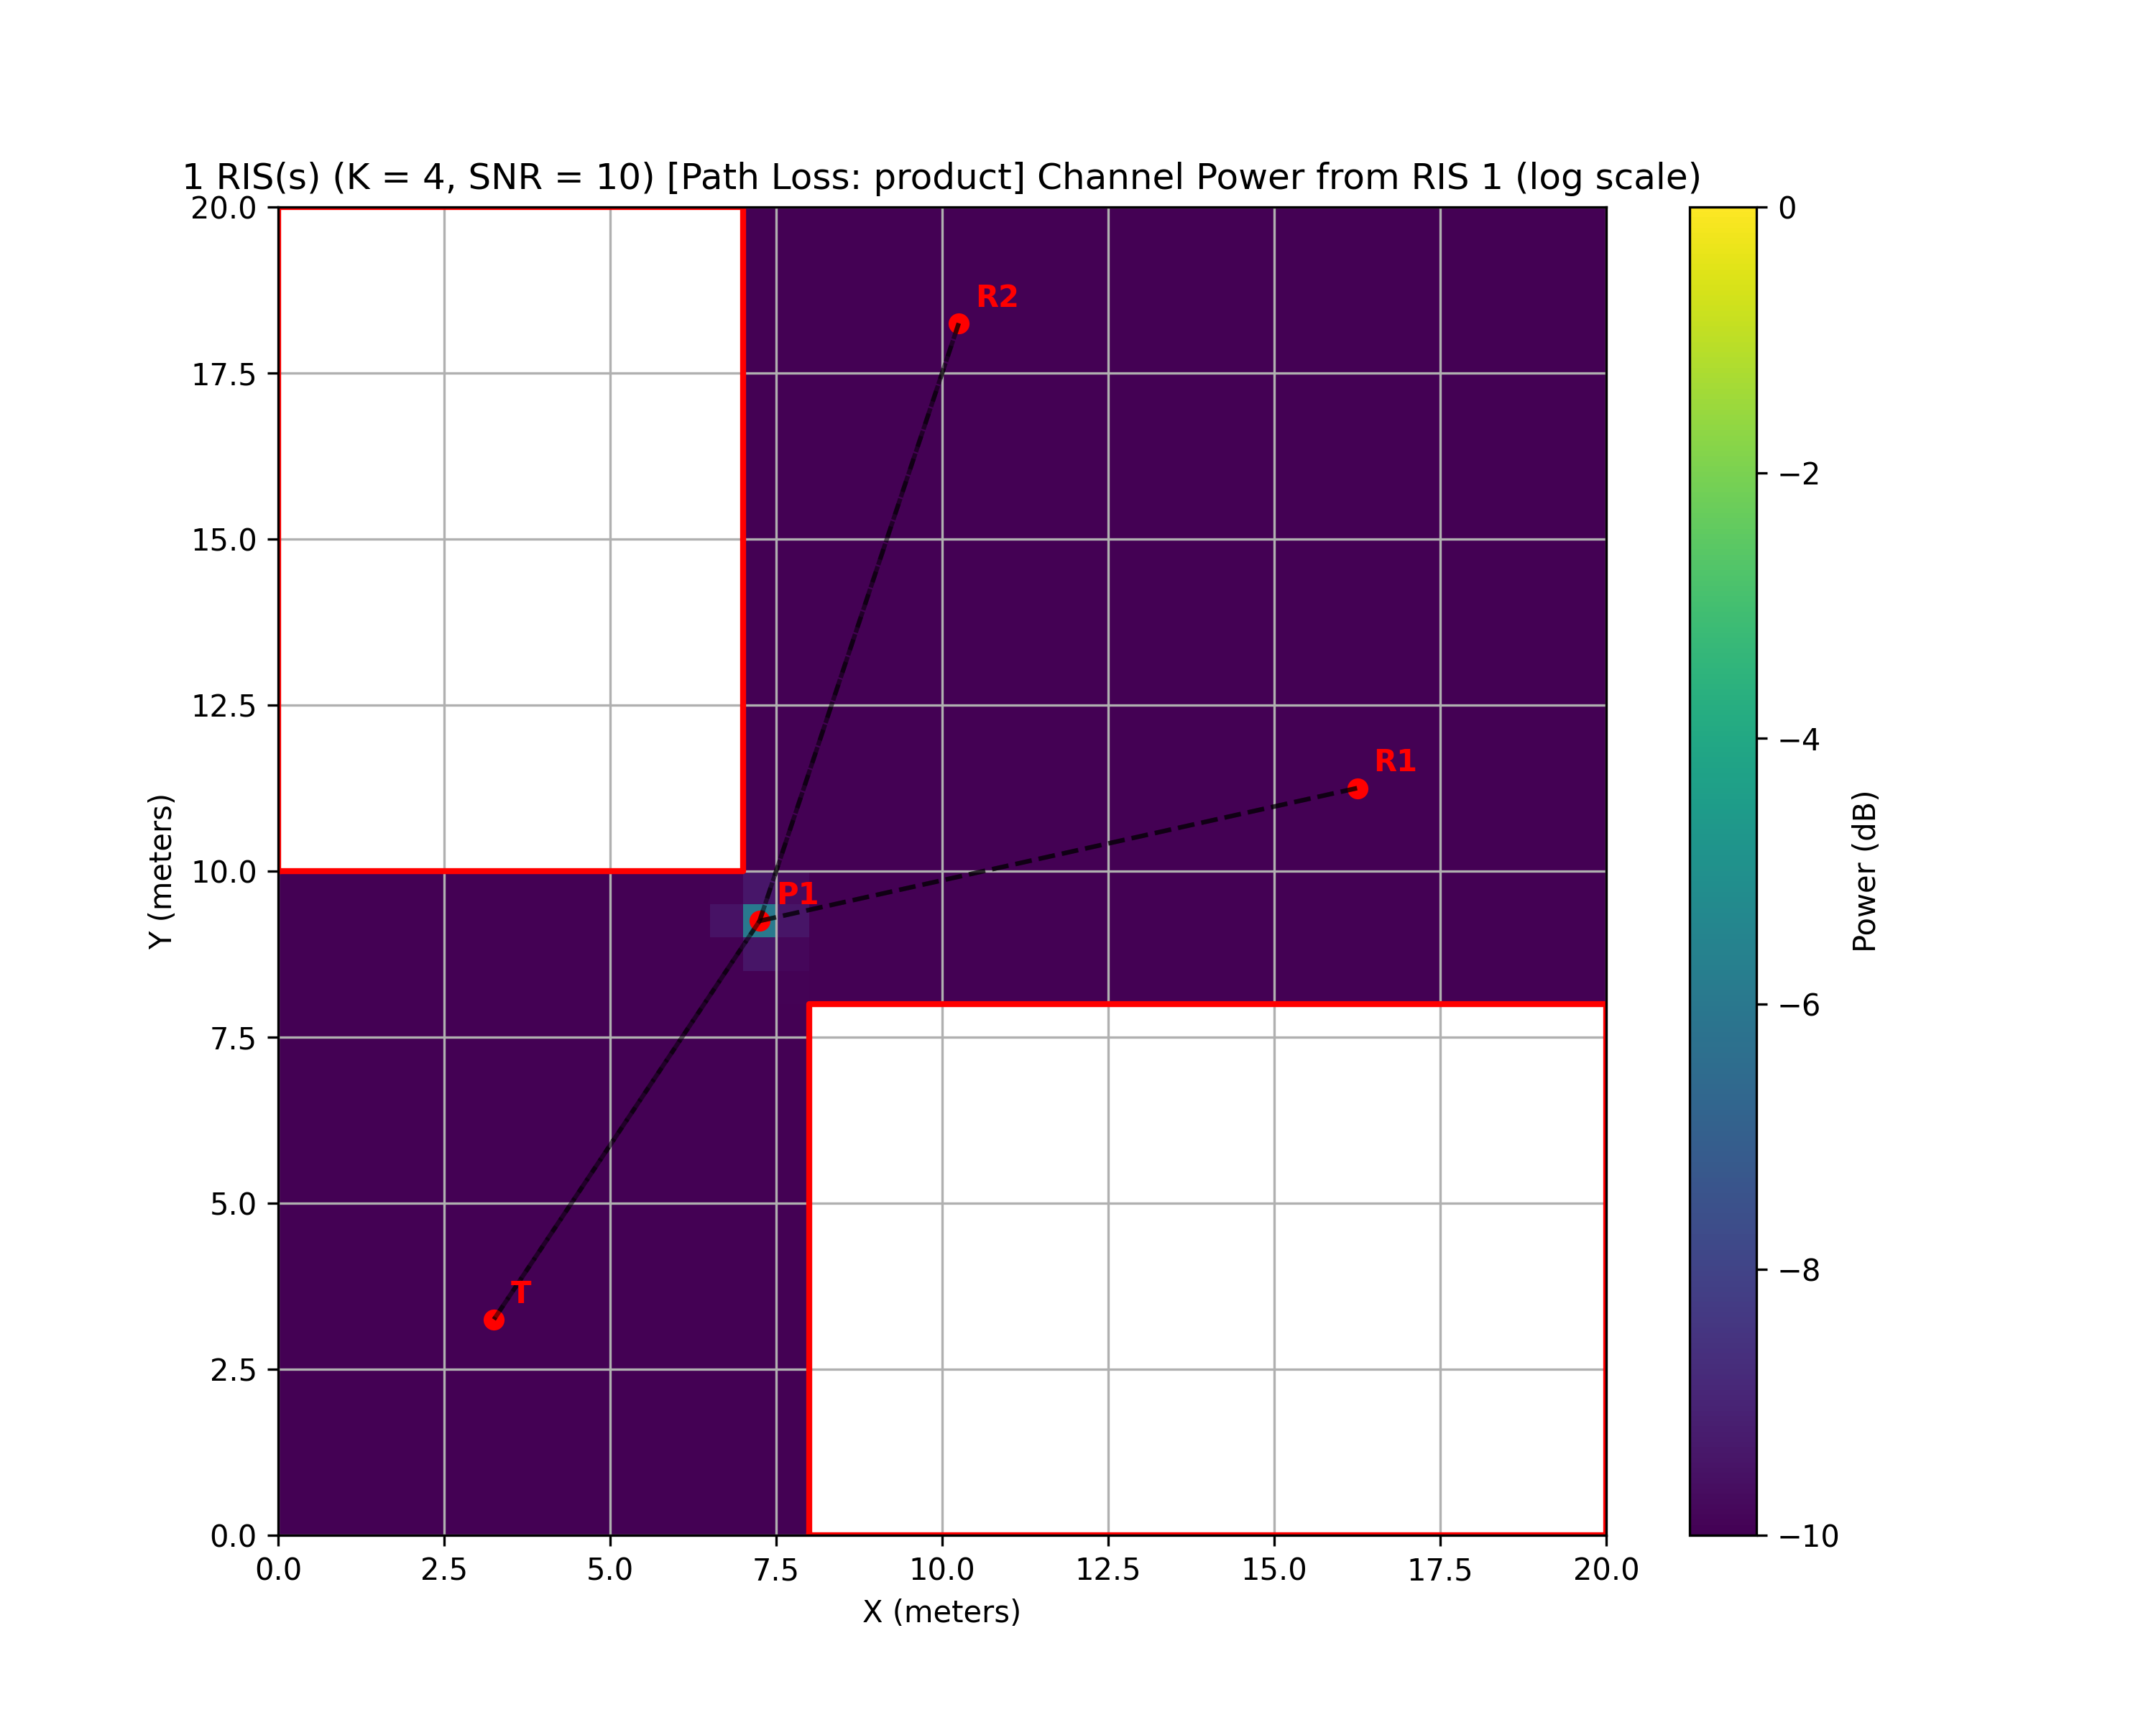
\includegraphics[width=0.7\linewidth]{imgs/heatmap-simulations/1 RIS(s) (K = 4, SNR = 10) [Path Loss_ product] Channel Power from RIS 1 (log scale).png}
  \caption{1 RIS(s) [Path Loss: product] Channel Power from RIS 1 (log scale)}
\end{figure}

\begin{figure}[H]
  \centering
  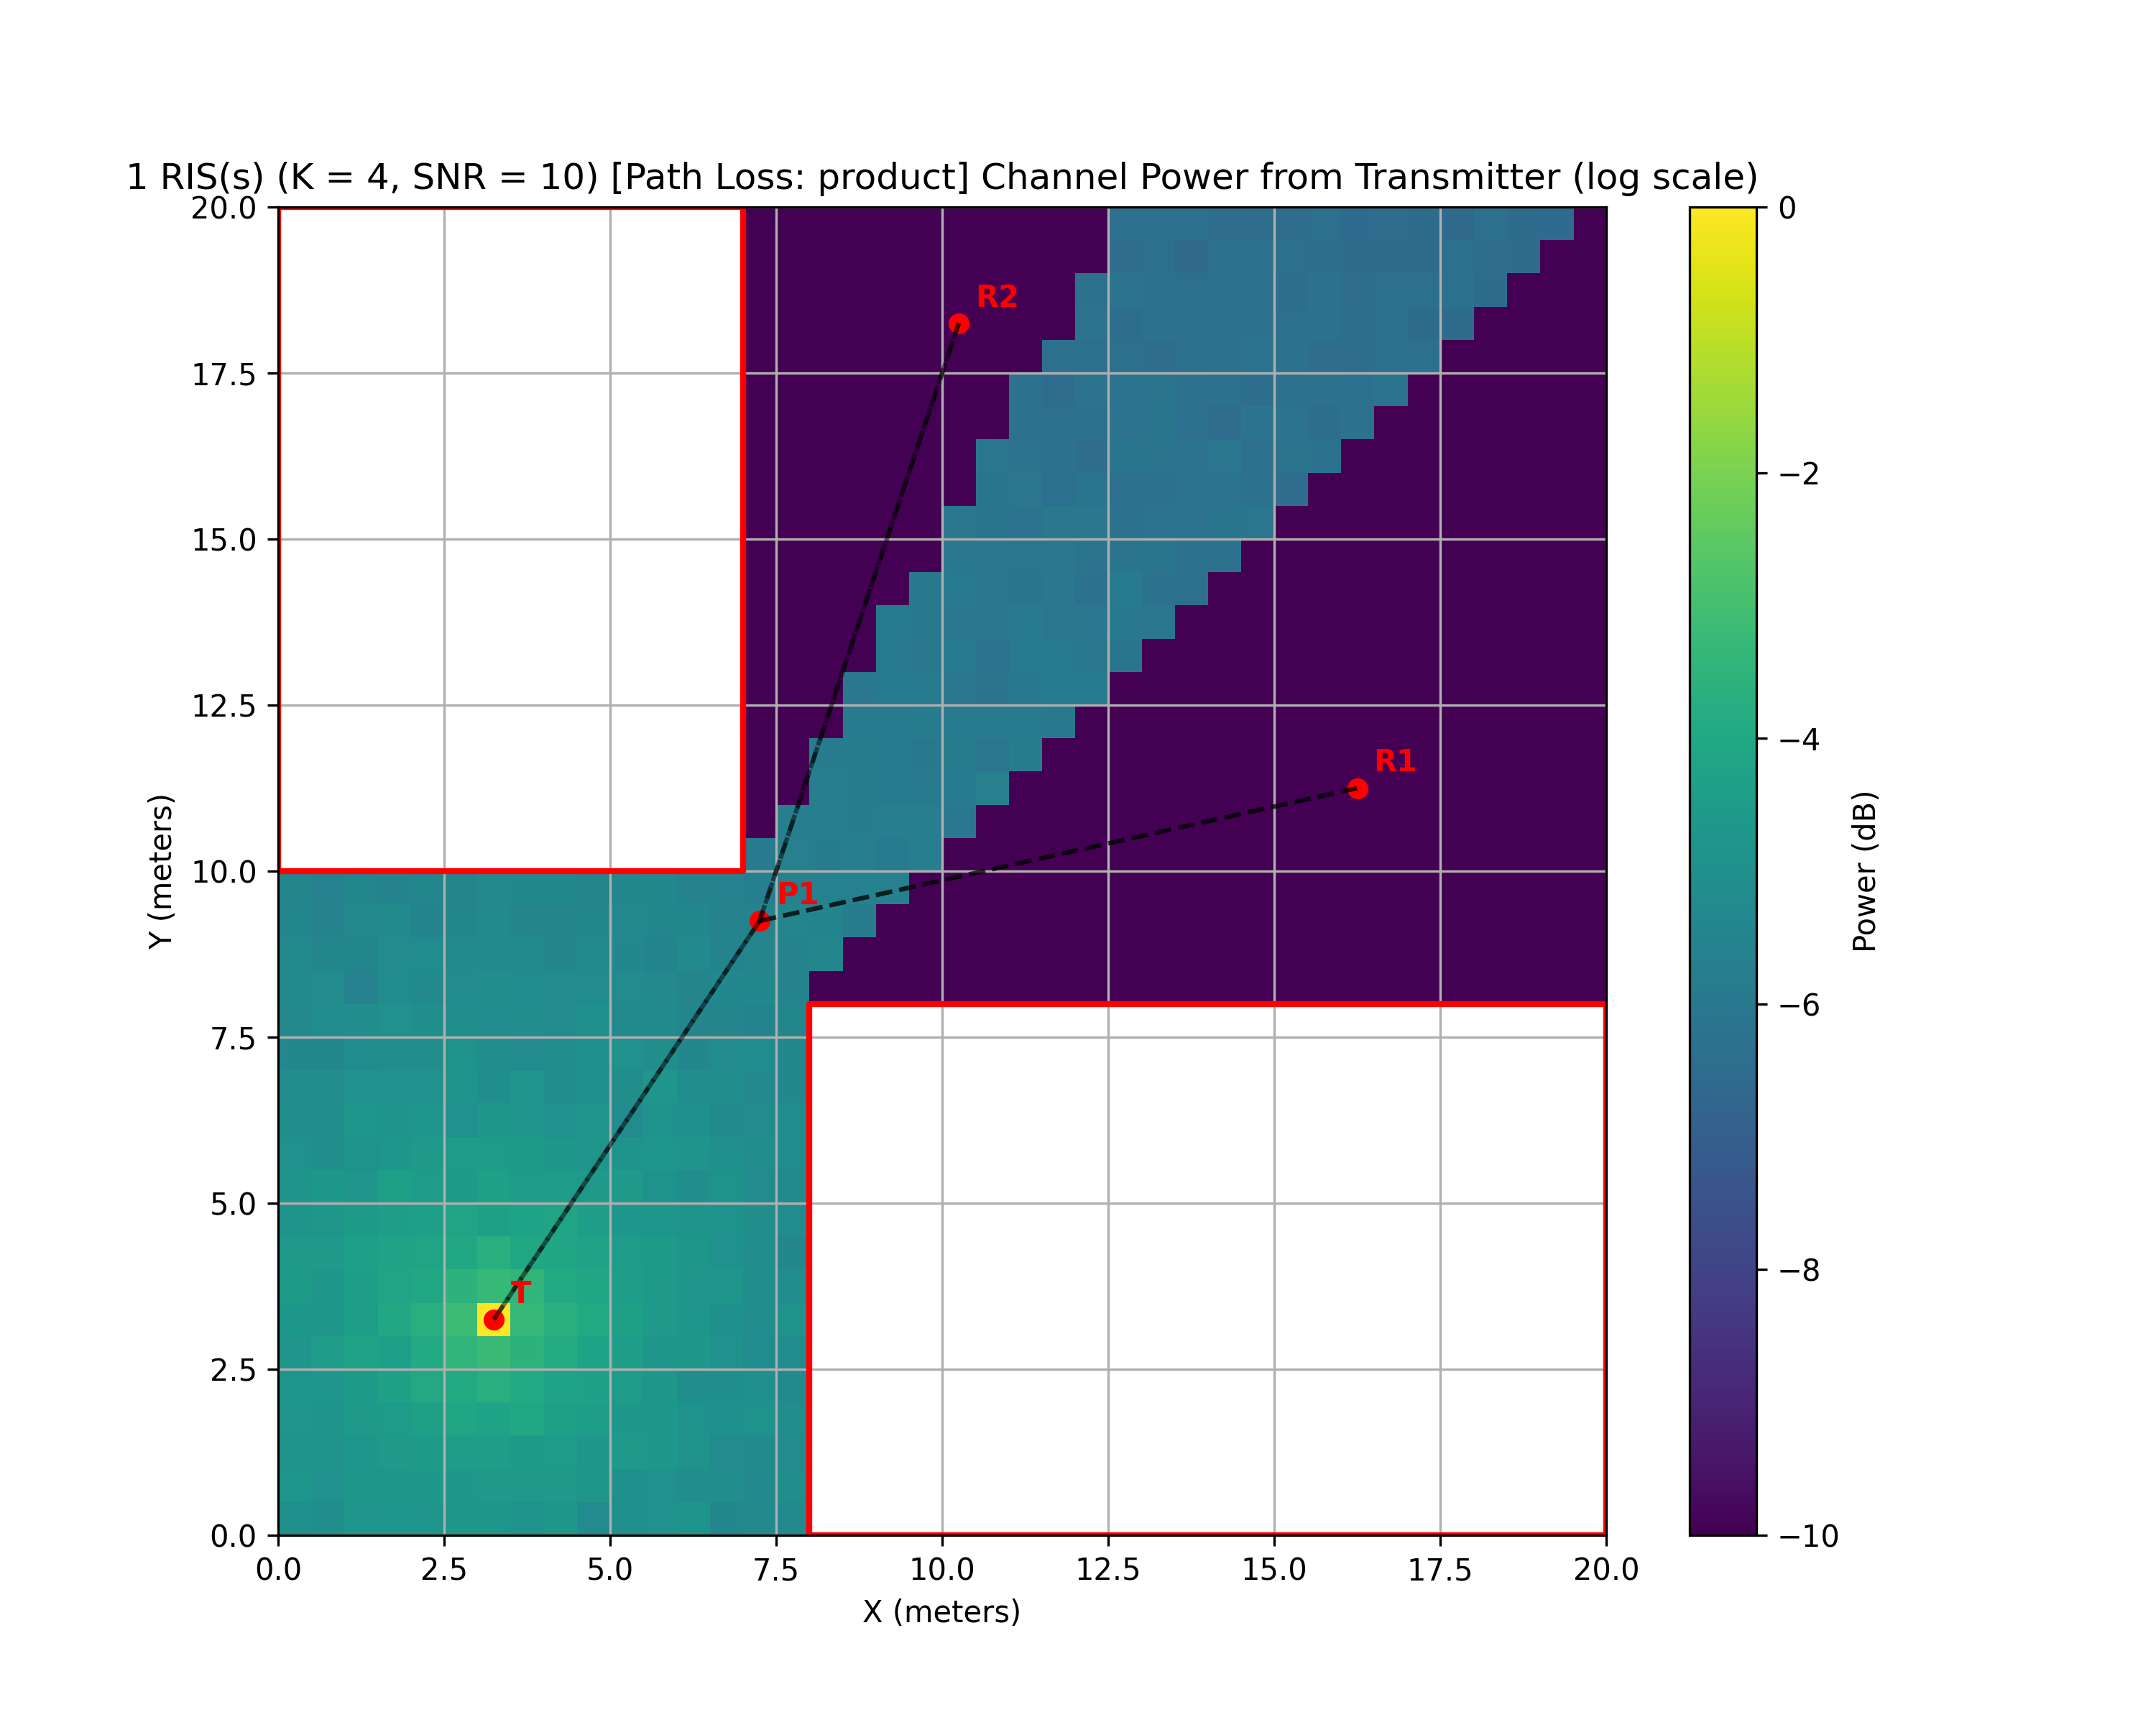
\includegraphics[width=0.7\linewidth]{imgs/heatmap-simulations/1 RIS(s) (K = 4, SNR = 10) [Path Loss_ product] Channel Power from Transmitter (log scale).png}
  \caption{1 RIS(s) [Path Loss: product] Channel Power from Transmitter (log scale)}
\end{figure}

\paragraph*{Path loss: sum}
This is the path loss that better confirms our previous BER analysis. Without LOS, the BER for eavesdropper is stable at 0.5, the same as random guessing. With LOS, the RIS is still able to influence significantly the outcome, with more noise that reduces the BER at 0.3

We can see how the power coming from the RIS reflection looks more uniform than the others. This is because, as we said before, this type of path loss actually models a directional RIS. The total result of this graph does not exist. You could see them as the union of all the possible graphs considering a single direction of the reflection.

\begin{figure}[H]
  \centering
  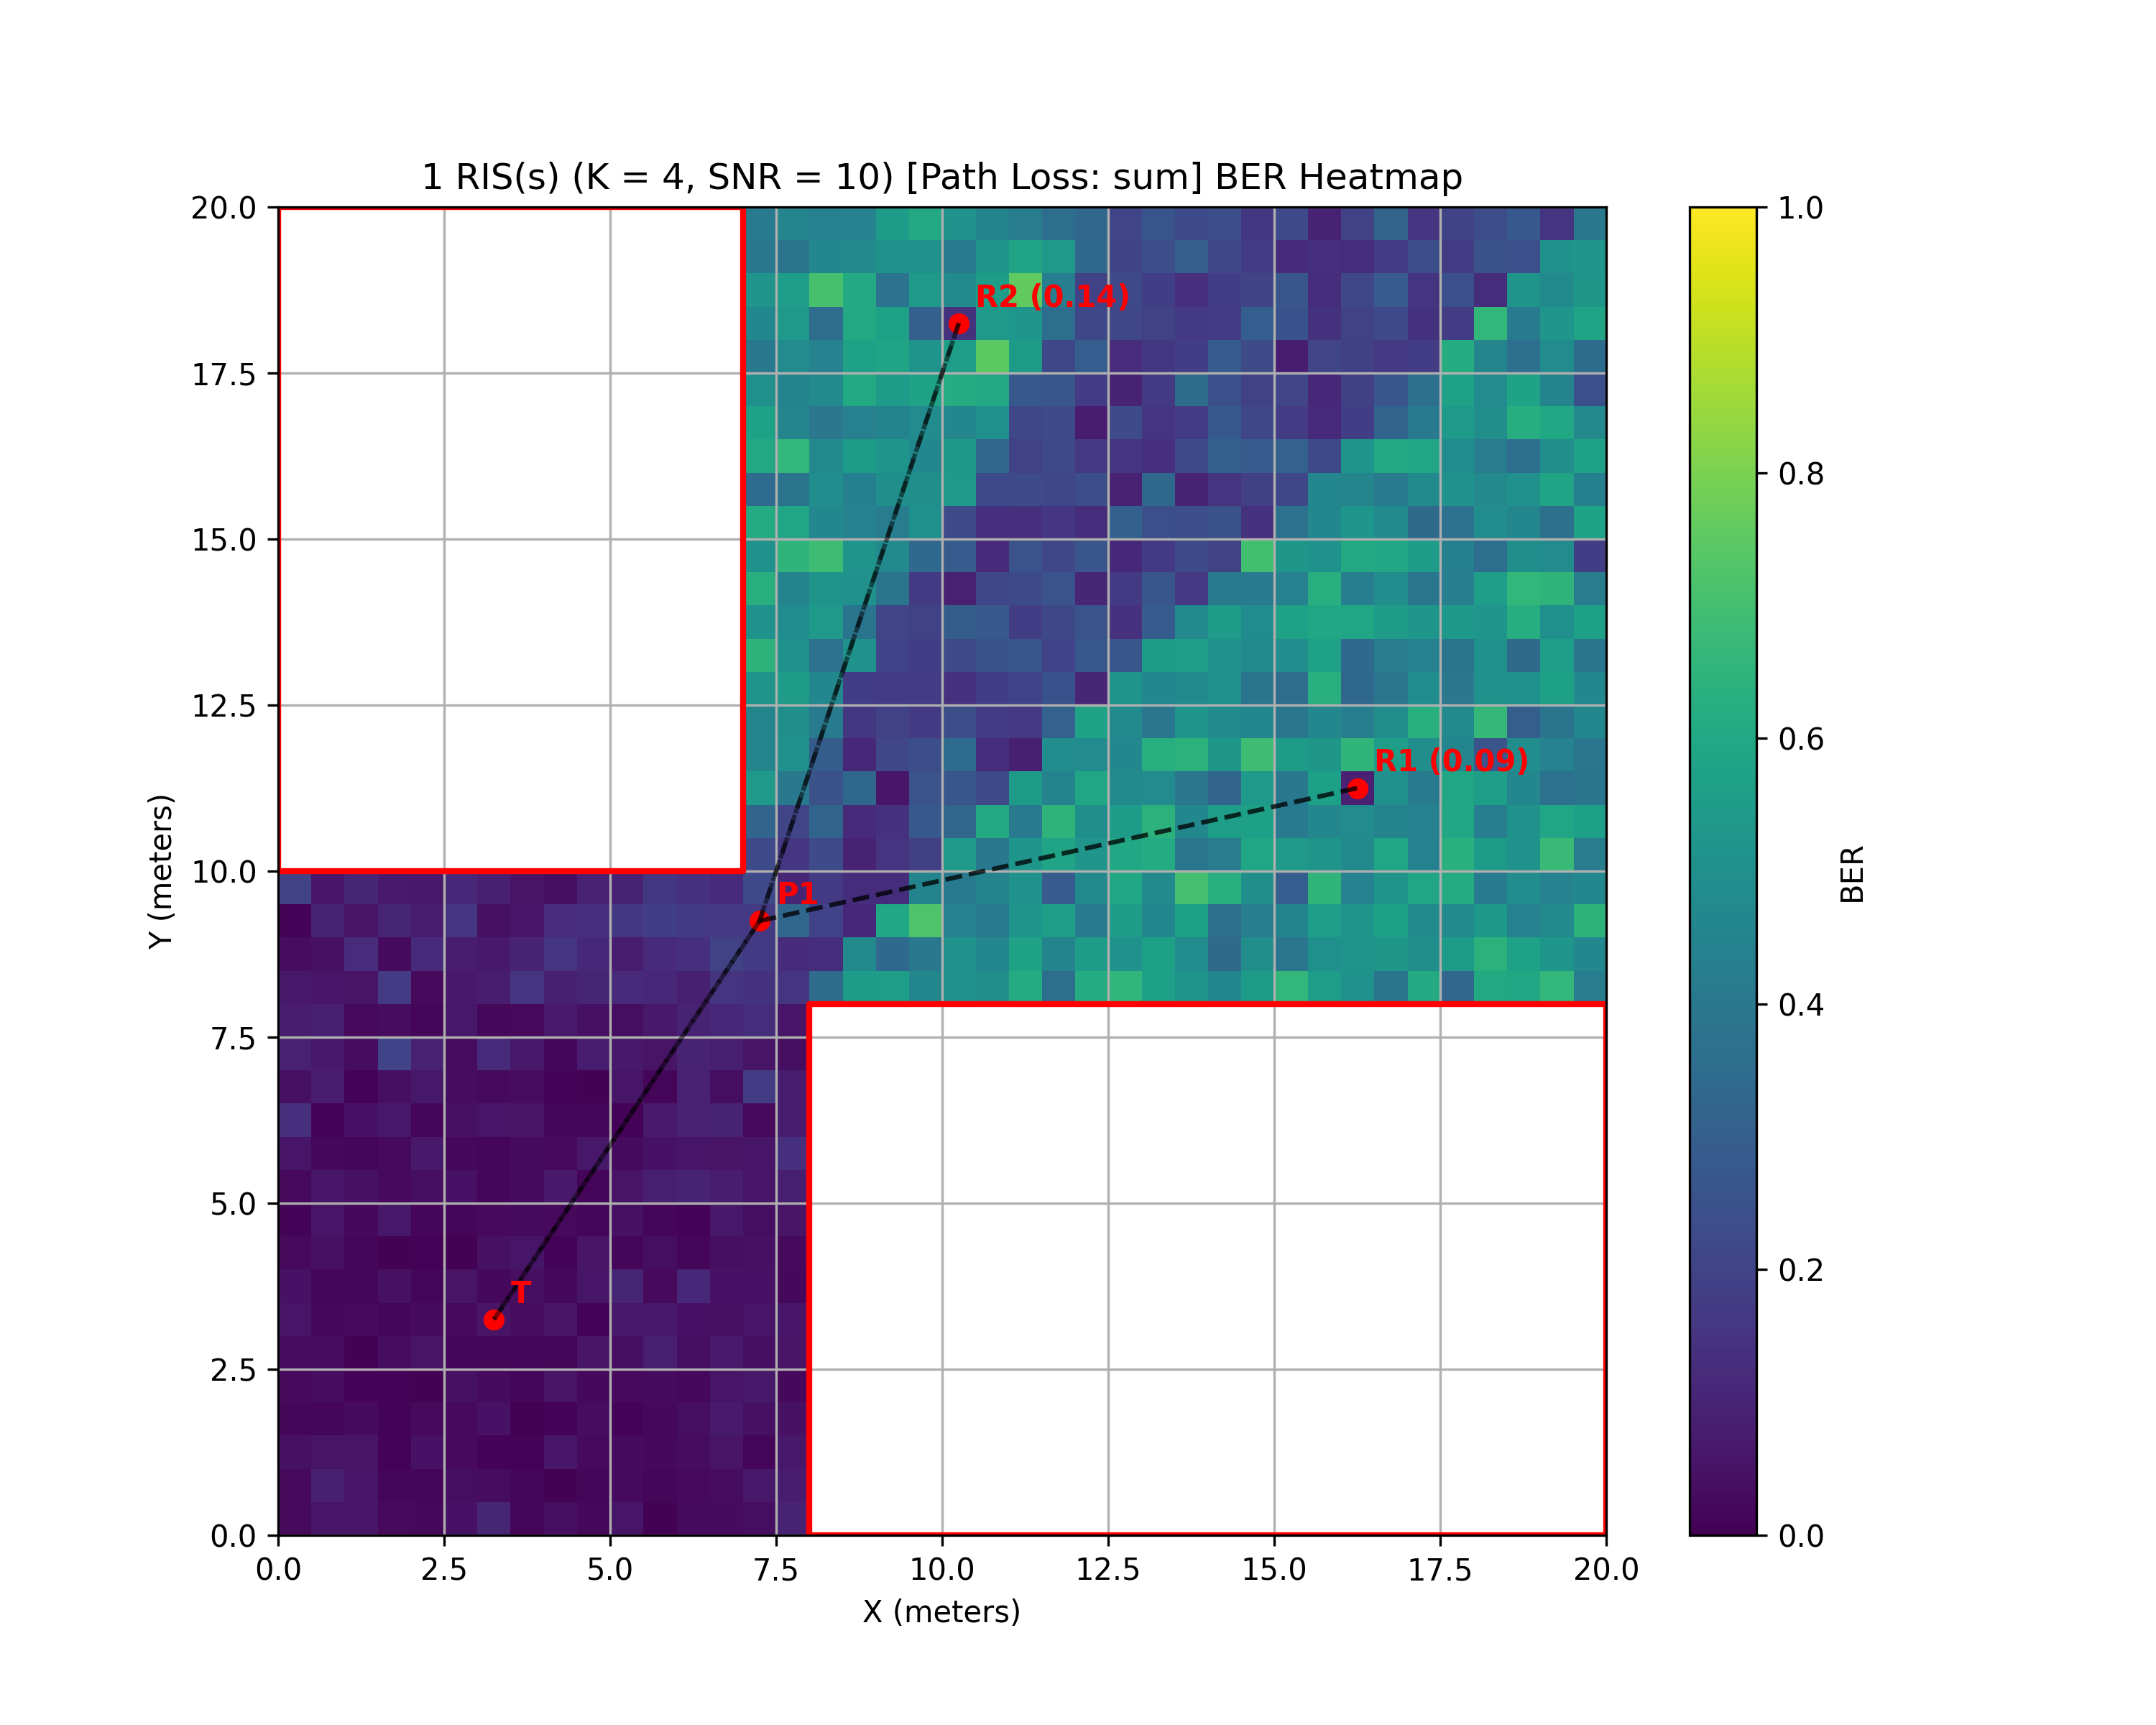
\includegraphics[width=0.7\linewidth]{imgs/heatmap-simulations/1 RIS(s) (K = 4, SNR = 10) [Path Loss_ sum] BER Heatmap.png}
  \caption{1 RIS(s) [Path Loss: sum] BER Heatmap}
\end{figure}

\begin{figure}[H]
  \centering
  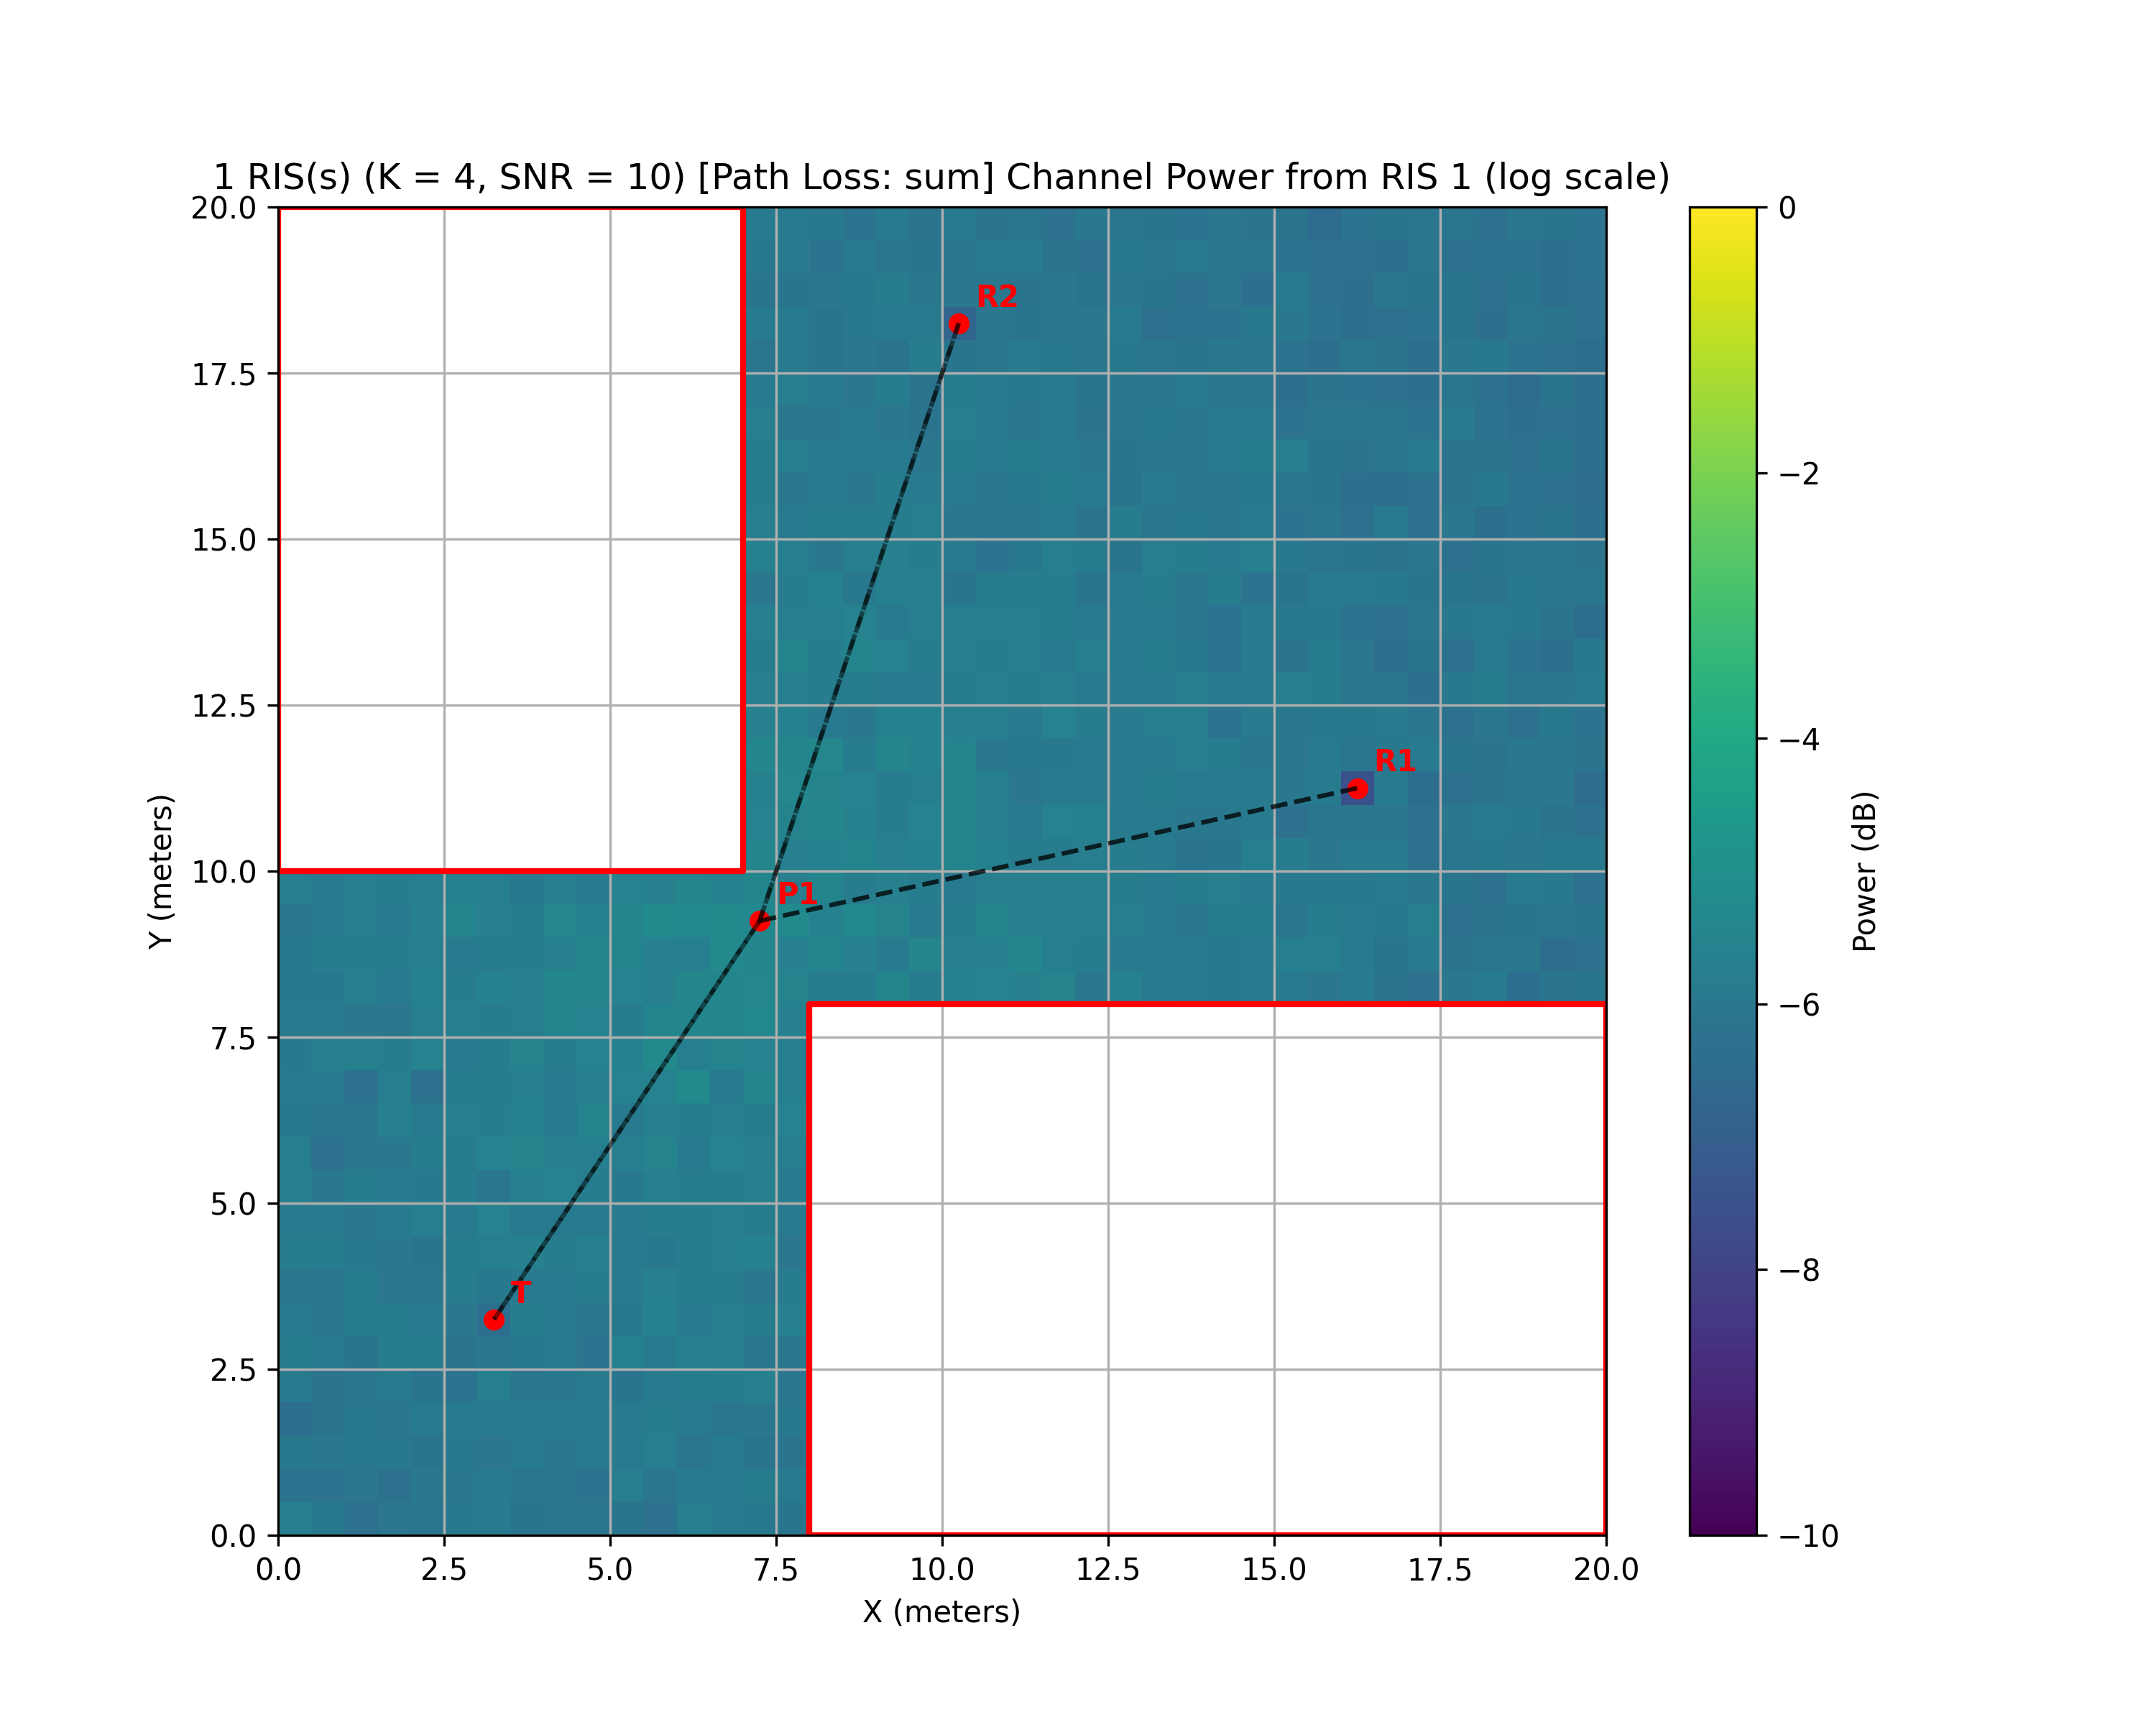
\includegraphics[width=0.7\linewidth]{imgs/heatmap-simulations/1 RIS(s) (K = 4, SNR = 10) [Path Loss_ sum] Channel Power from RIS 1 (log scale).png}
  \caption{1 RIS(s) [Path Loss: sum] Channel Power from RIS 1 (log scale)}
\end{figure}

\begin{figure}[H]
  \centering
  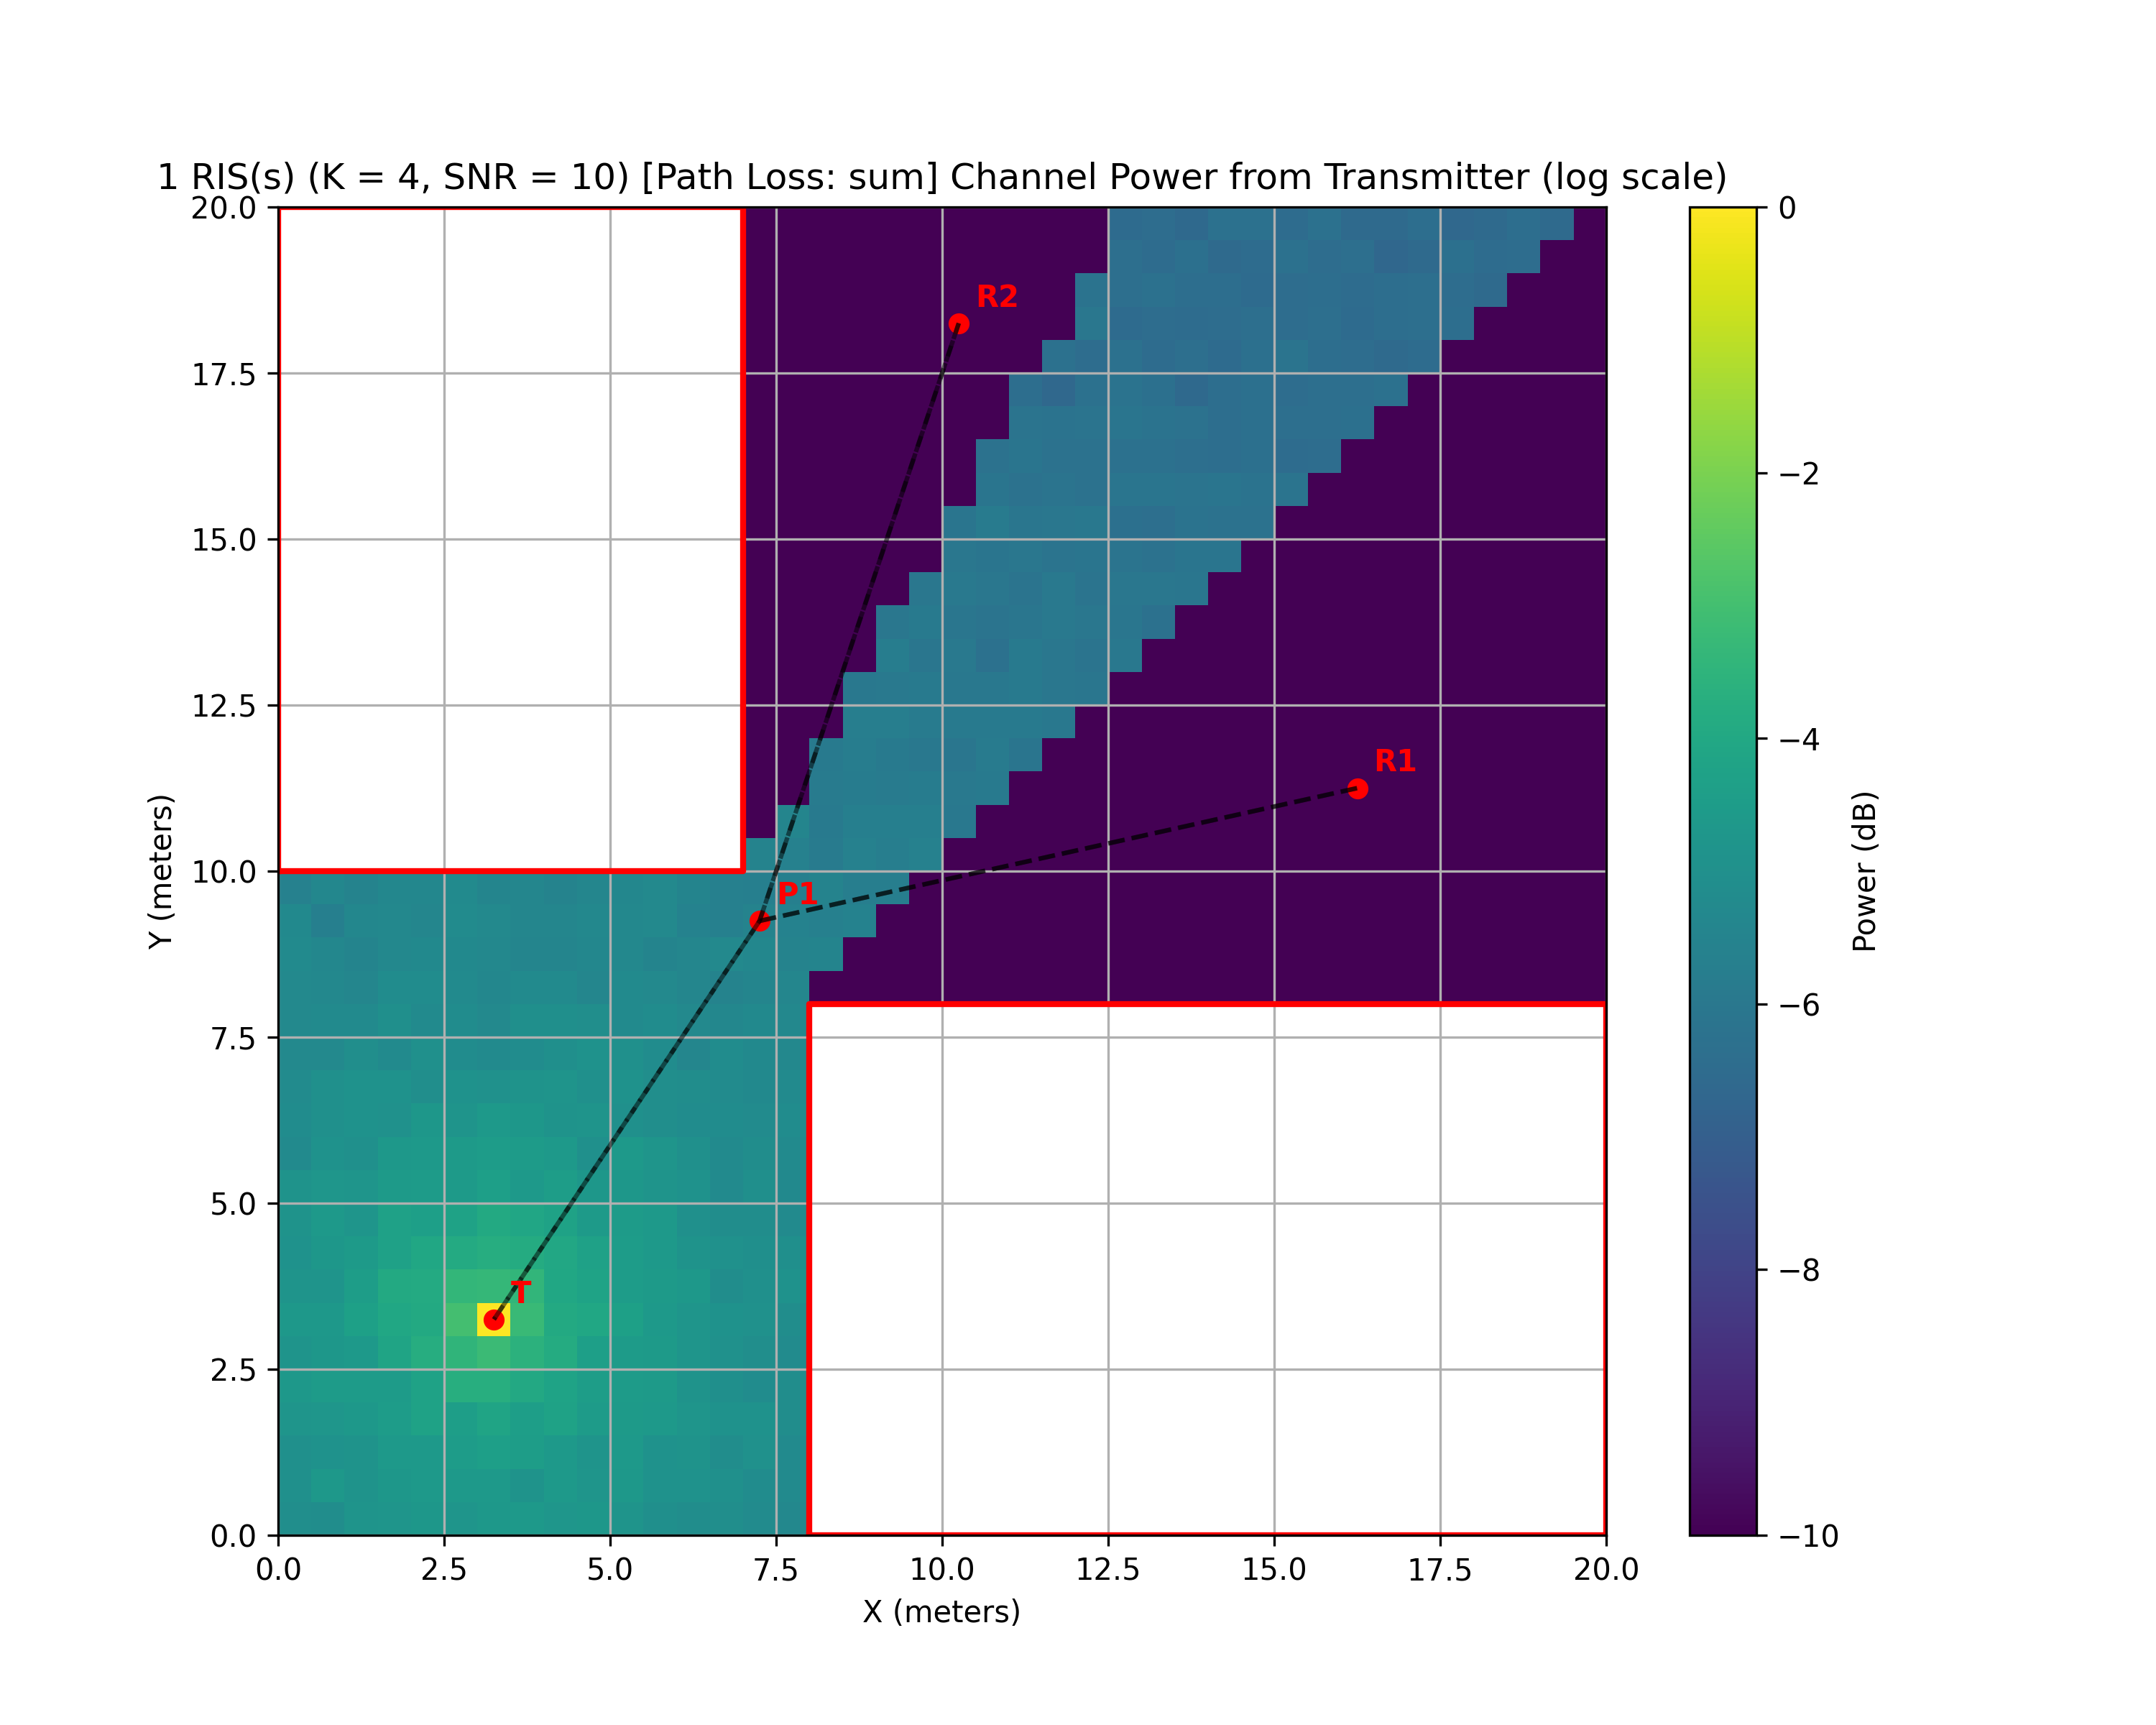
\includegraphics[width=0.7\linewidth]{imgs/heatmap-simulations/1 RIS(s) (K = 4, SNR = 10) [Path Loss_ sum] Channel Power from Transmitter (log scale).png}
  \caption{1 RIS(s) [Path Loss: sum] Channel Power from Transmitter (log scale)}
\end{figure}

\subsubsection{Double reflection from 2 RIS in series}

It is certainly interesting to also study what would happen if we concatenate two RIS in series in relation to their combined path loss. For these tests, we used $\lambda = 0.08m, \tau = 0.6, \xi = 1, \eta = 0.9, SNR = 10db, K = 2, N = 16$.

All scenarios suppose the RIS use the same kind of path loss, meaning they are of different kind (active, passive uniform, passive directional). Of course, it would be an interesting case studying combining different variations of them to reach the most cost and power - efficient configuration.

Additional scenarios with RIS in parallel would also be valuable for future research, as they would likely show promising security characteristics based on our preliminary analysis.

\paragraph*{Path loss: active}
Similar to the previous scenario, we can clearly see where the RIS have significant power to influence the signal reception, and where without LOS the signal is undecipherable for eavesdroppers.

As said before, it is slightly visible where the direct signal from \textbf{T} is and is not present. It is not visible however the difference where only \textbf{P2} creates interference from where both \textbf{P1} and \textbf{P2} contribute to the noise. You could imagine the area by selecting the intersection between the two RIS Channel Power graphs.

\begin{figure}[H]
  \centering
  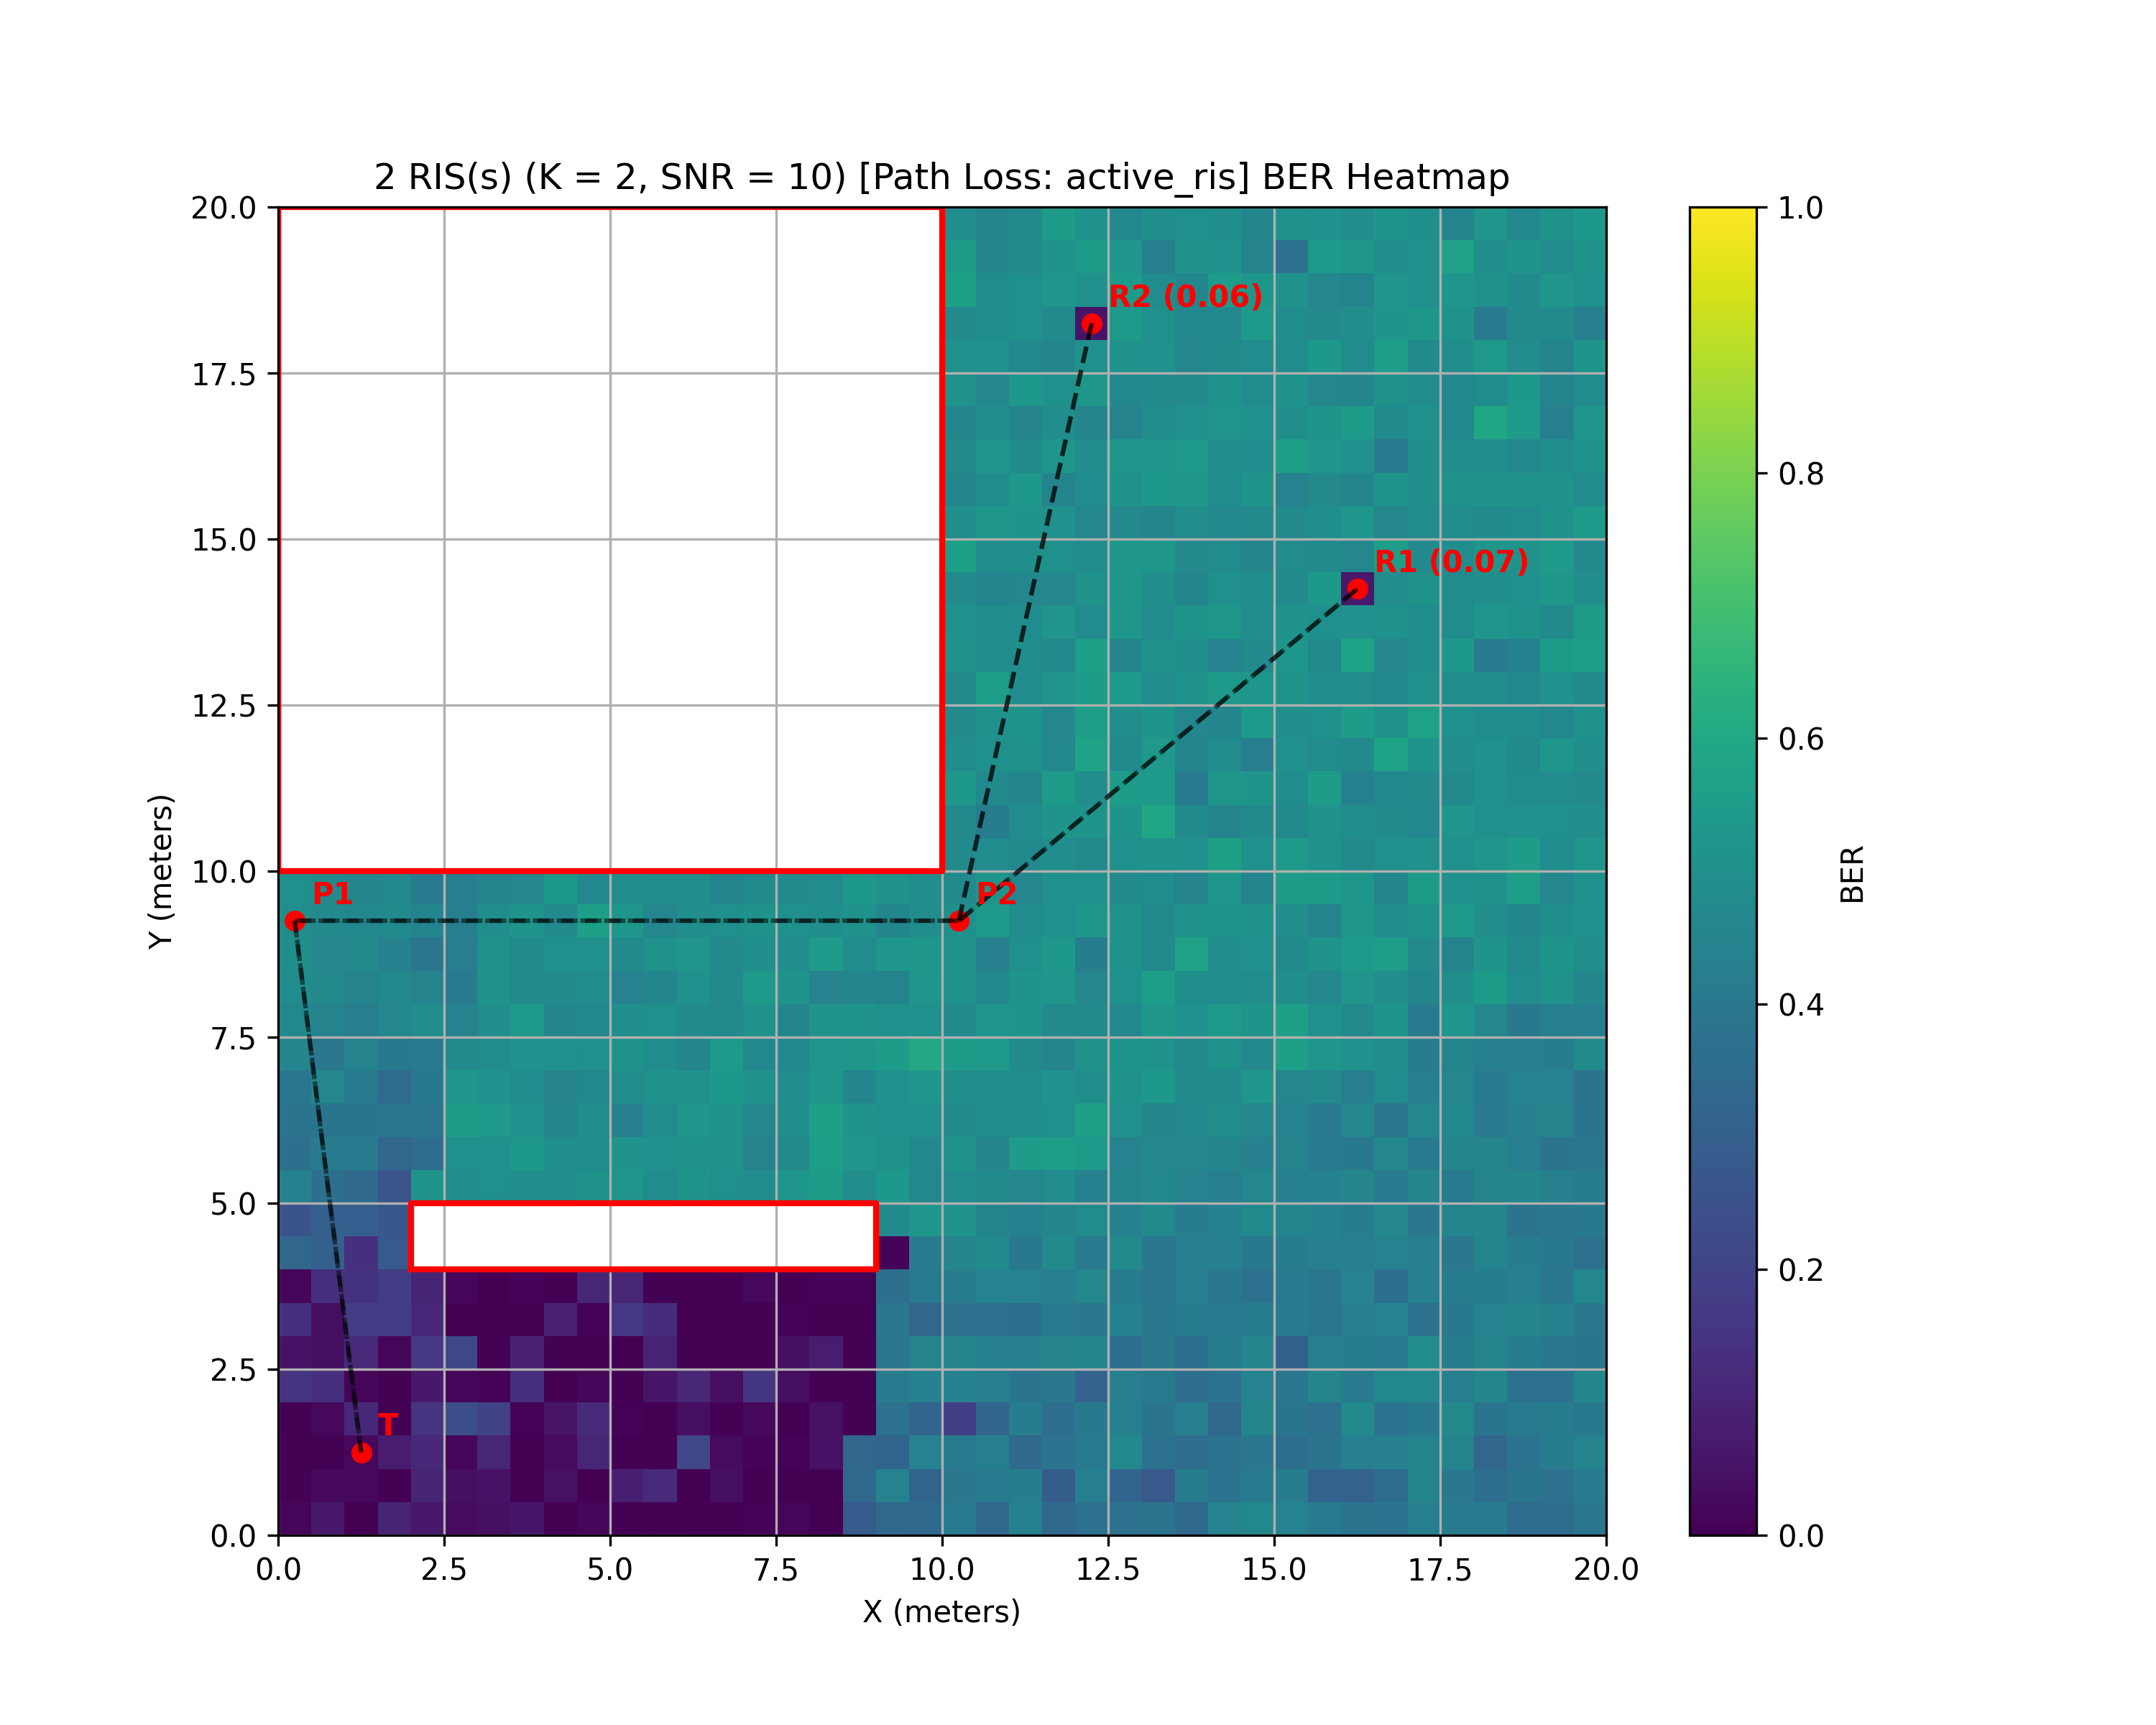
\includegraphics[width=0.7\linewidth]{imgs/heatmap-simulations/2 RIS(s) (K = 2, SNR = 10) [Path Loss_ active_ris] BER Heatmap.png}
  \caption{2 RIS(s) [Path Loss: active ris] BER Heatmap}
\end{figure}

\begin{figure}[H]
  \centering
  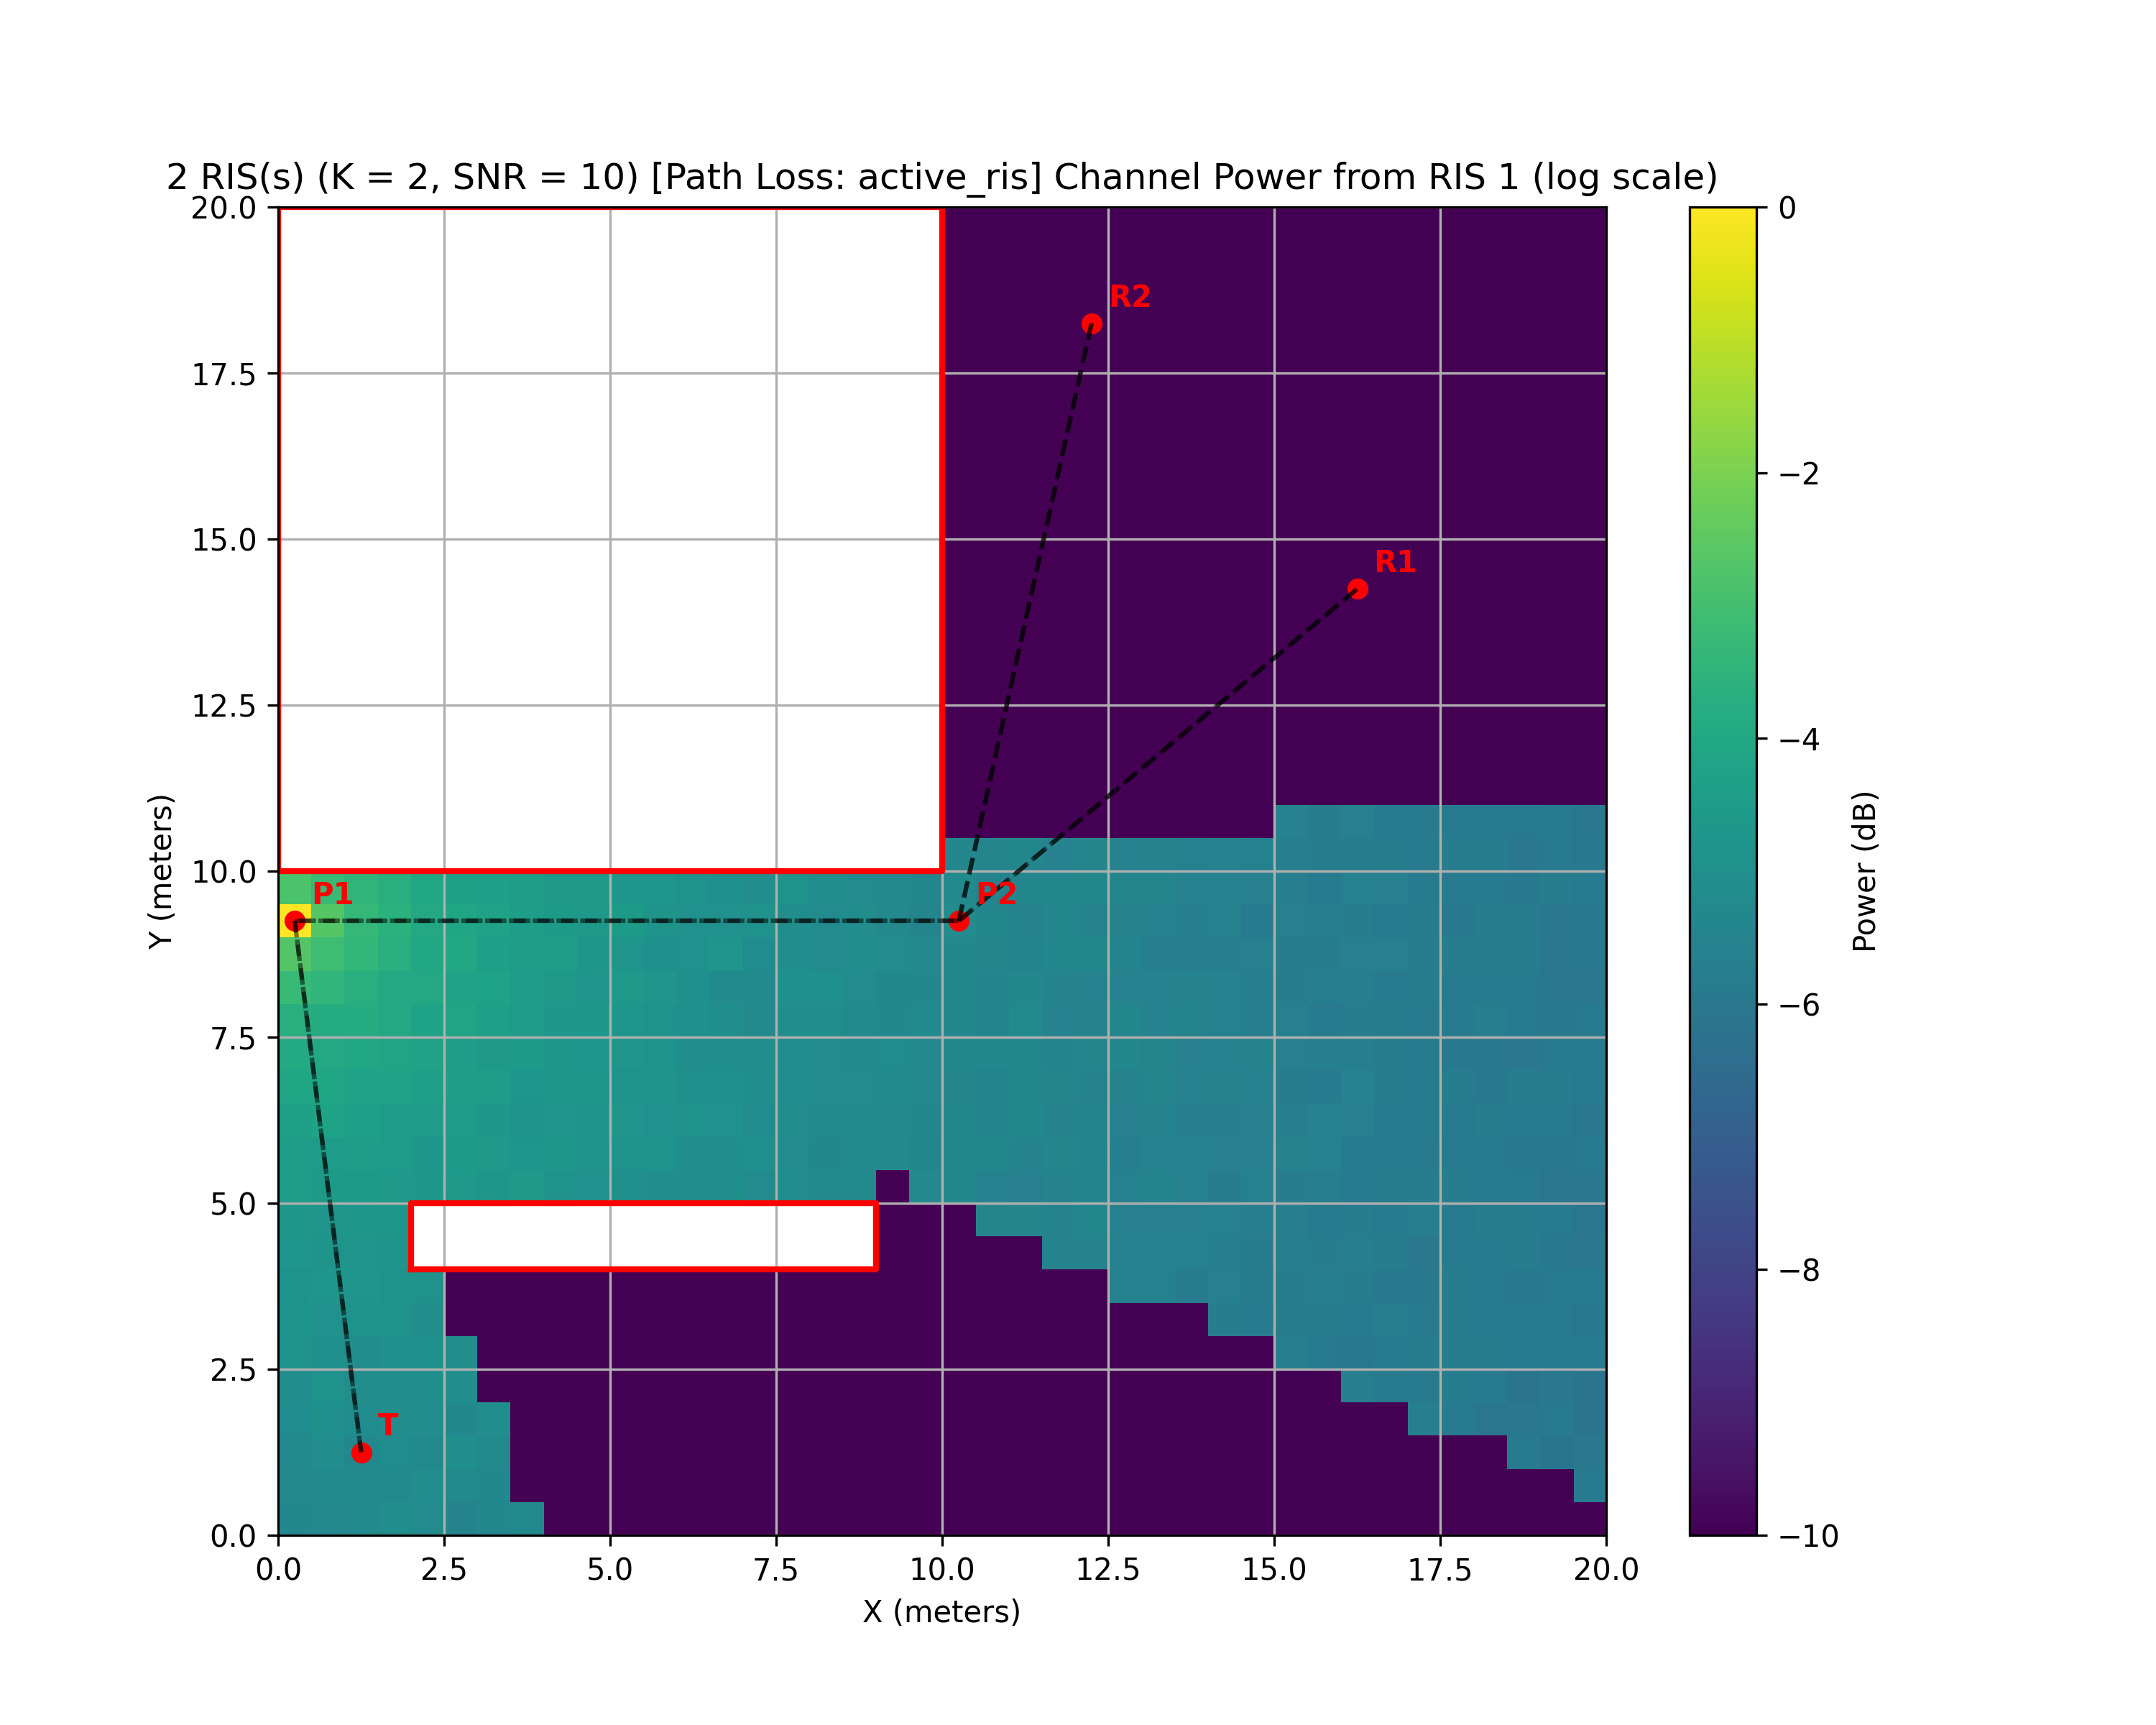
\includegraphics[width=0.7\linewidth]{imgs/heatmap-simulations/2 RIS(s) (K = 2, SNR = 10) [Path Loss_ active_ris] Channel Power from RIS 1 (log scale).png}
  \caption{2 RIS(s) [Path Loss: active ris] Channel Power from RIS 1 (log scale)}
\end{figure}

\begin{figure}[H]
  \centering
  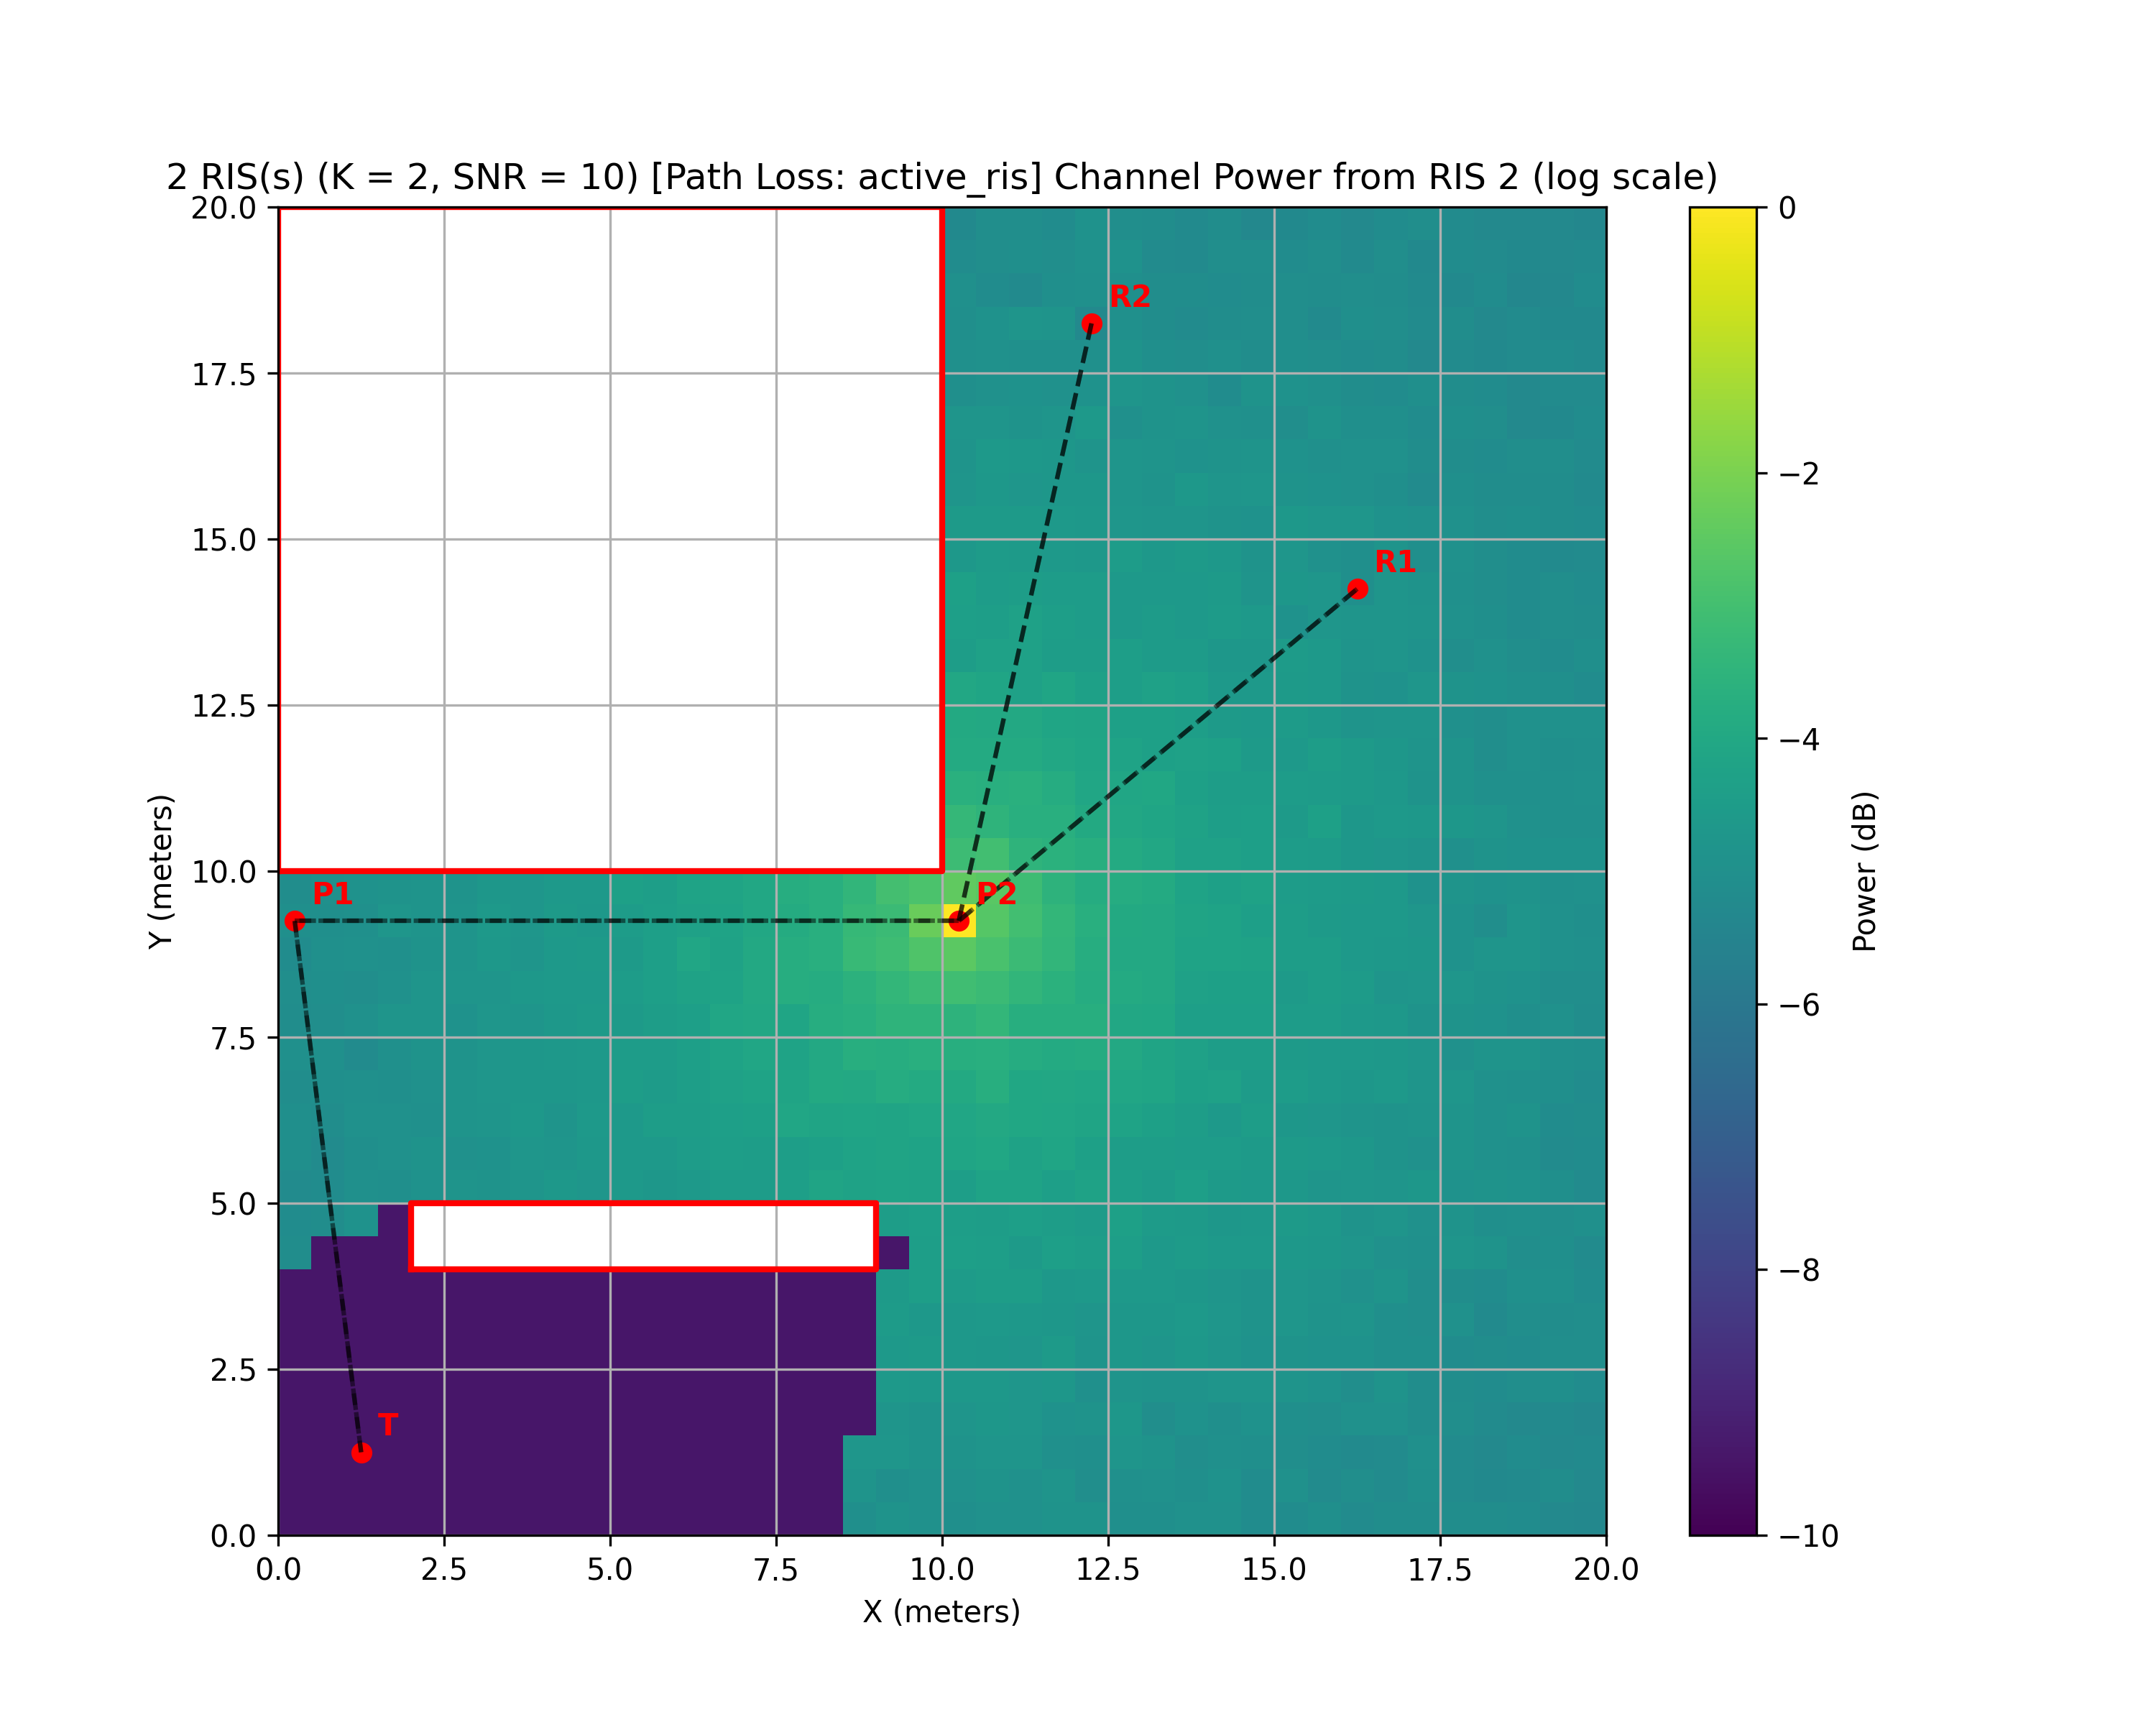
\includegraphics[width=0.7\linewidth]{imgs/heatmap-simulations/2 RIS(s) (K = 2, SNR = 10) [Path Loss_ active_ris] Channel Power from RIS 2 (log scale).png}
  \caption{2 RIS(s) [Path Loss: active ris] Channel Power from RIS 2 (log scale)}
\end{figure}

\begin{figure}[H]
  \centering
  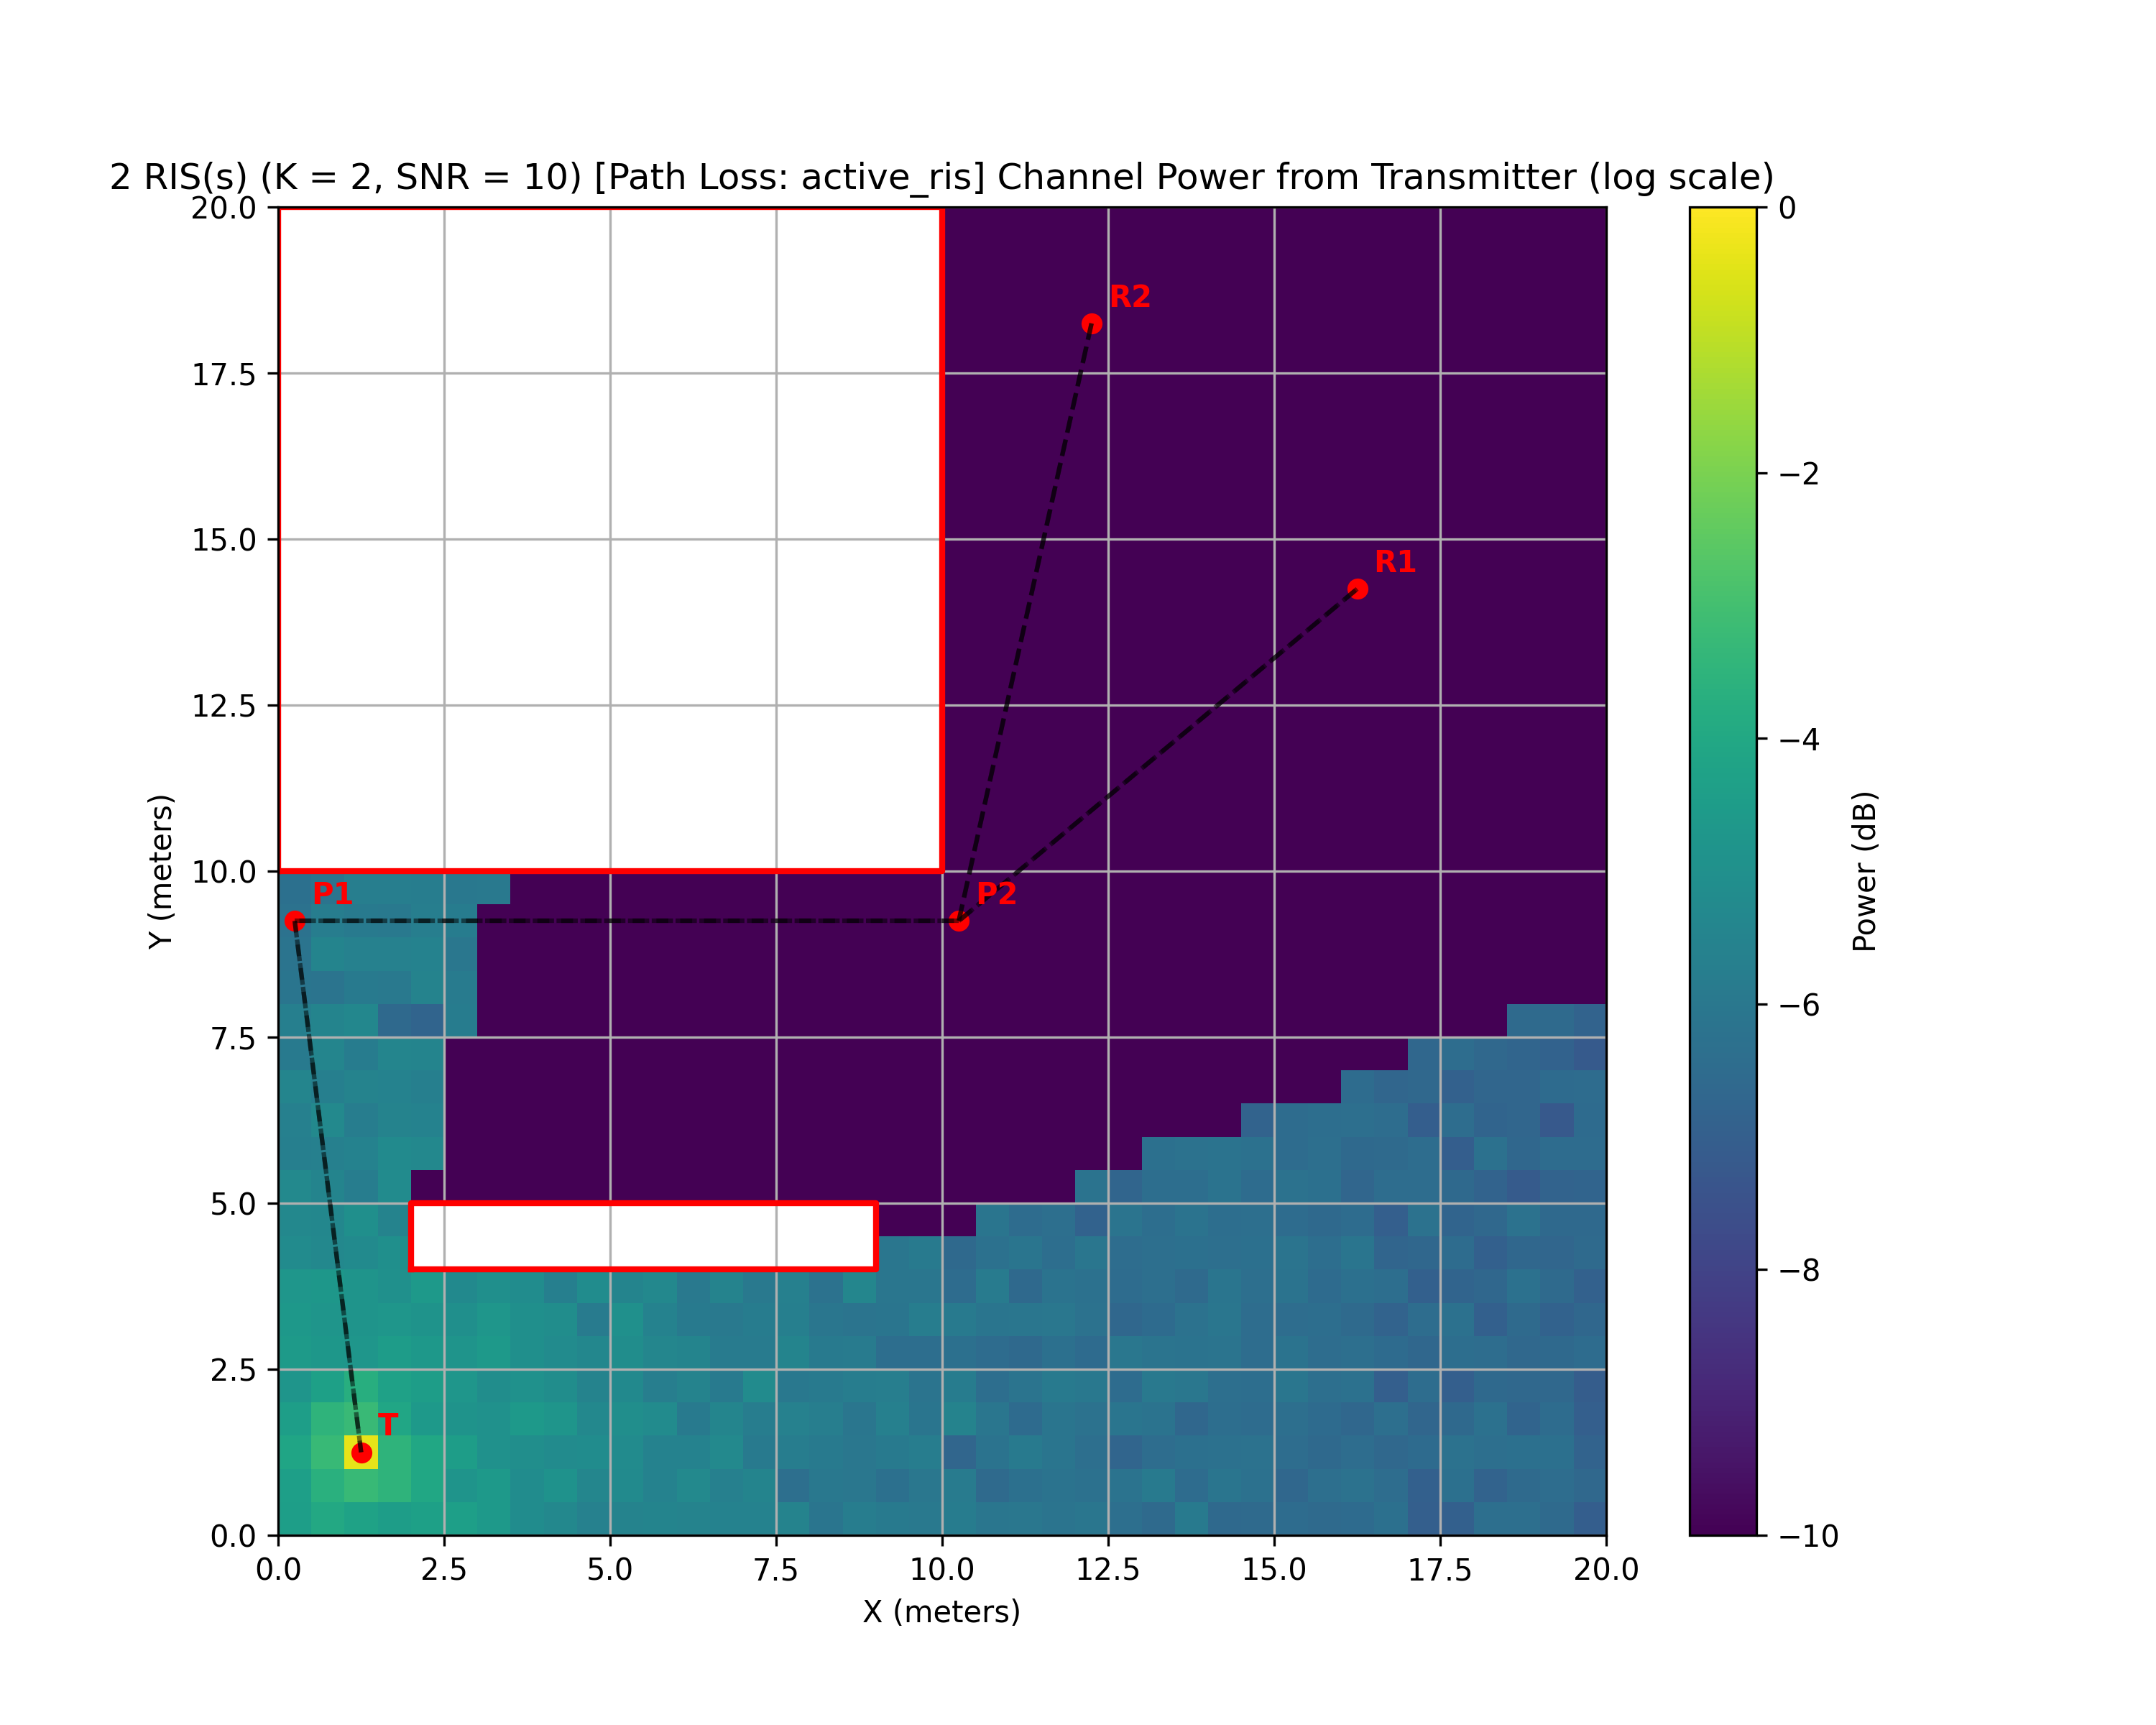
\includegraphics[width=0.7\linewidth]{imgs/heatmap-simulations/2 RIS(s) (K = 2, SNR = 10) [Path Loss_ active_ris] Channel Power from Transmitter (log scale).png}
  \caption{2 RIS(s) [Path Loss: active ris] Channel Power from Transmitter (log scale)}
\end{figure}

\paragraph*{Path loss: product}
We can draw similar conclusions as before for the product path loss. As we can see, the direct signal is not disturbed, and the reflection from \textbf{P2} after being already reflected from \textbf{P1} is so low, it does not even show on the \textbf{P2} position itself.

\begin{figure}[H]
  \centering
  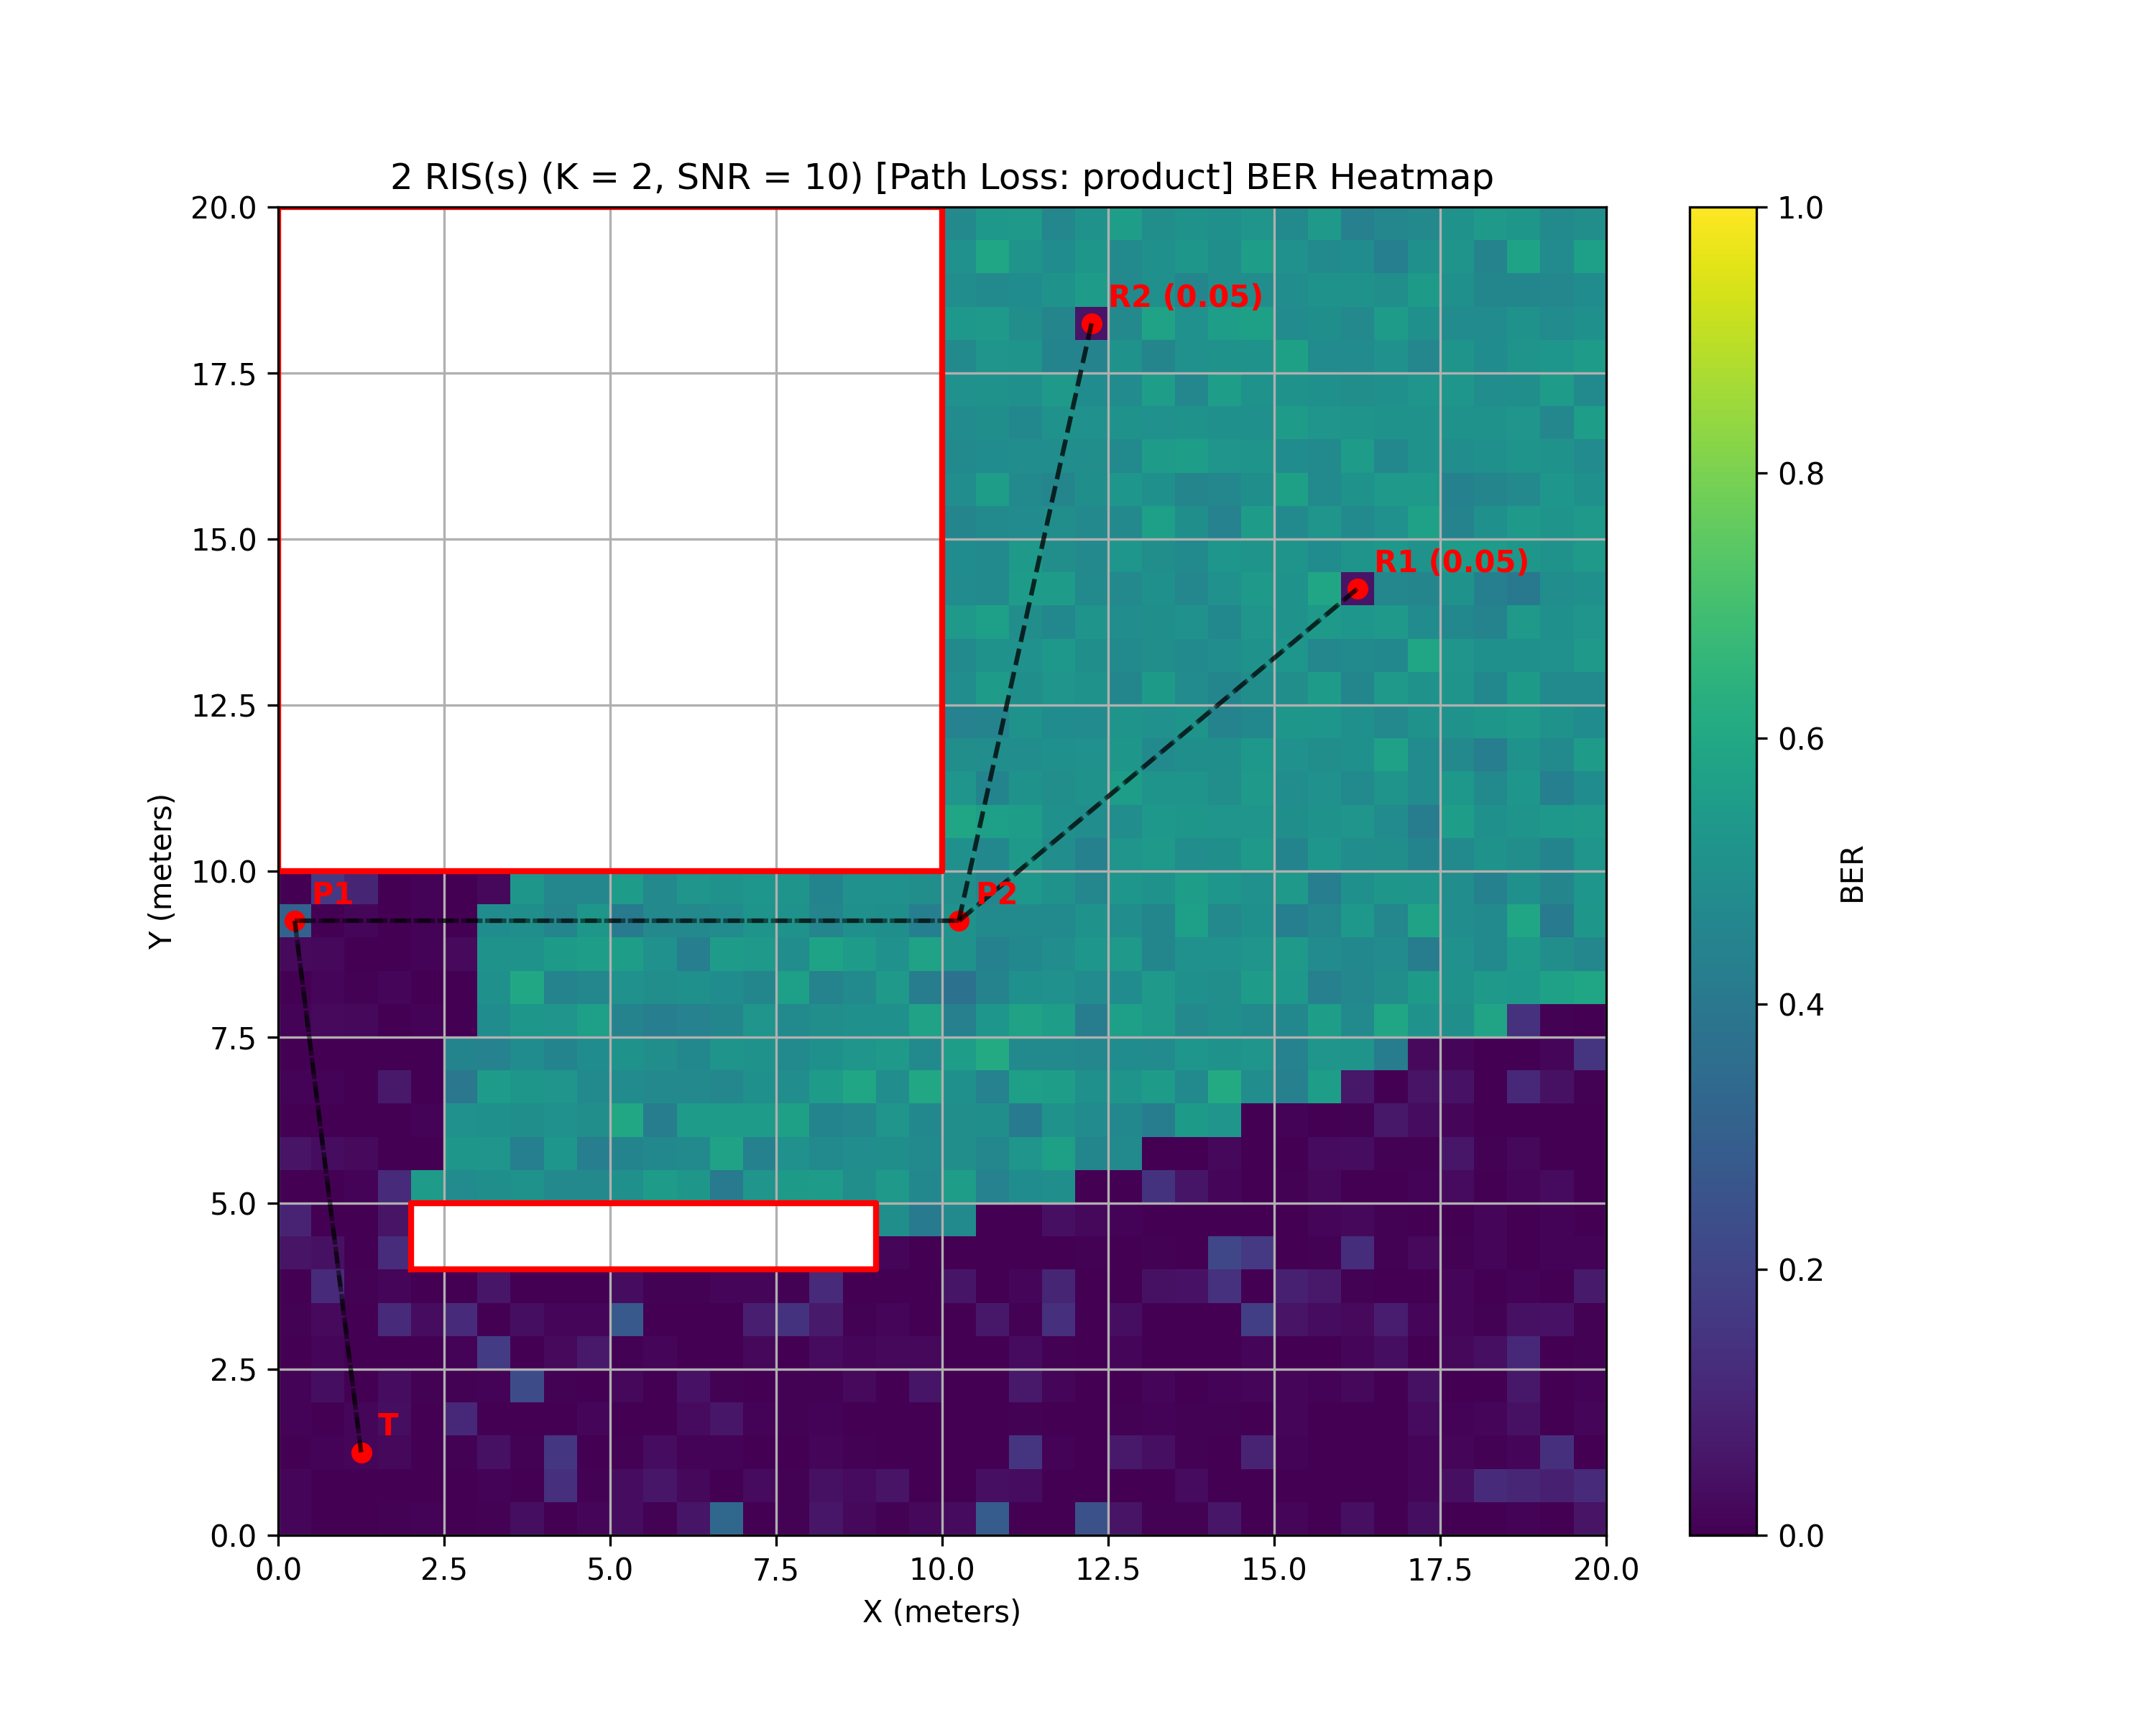
\includegraphics[width=0.7\linewidth]{imgs/heatmap-simulations/2 RIS(s) (K = 2, SNR = 10) [Path Loss_ product] BER Heatmap.png}
  \caption{2 RIS(s) [Path Loss: product] BER Heatmap}
\end{figure}

\begin{figure}[H]
  \centering
  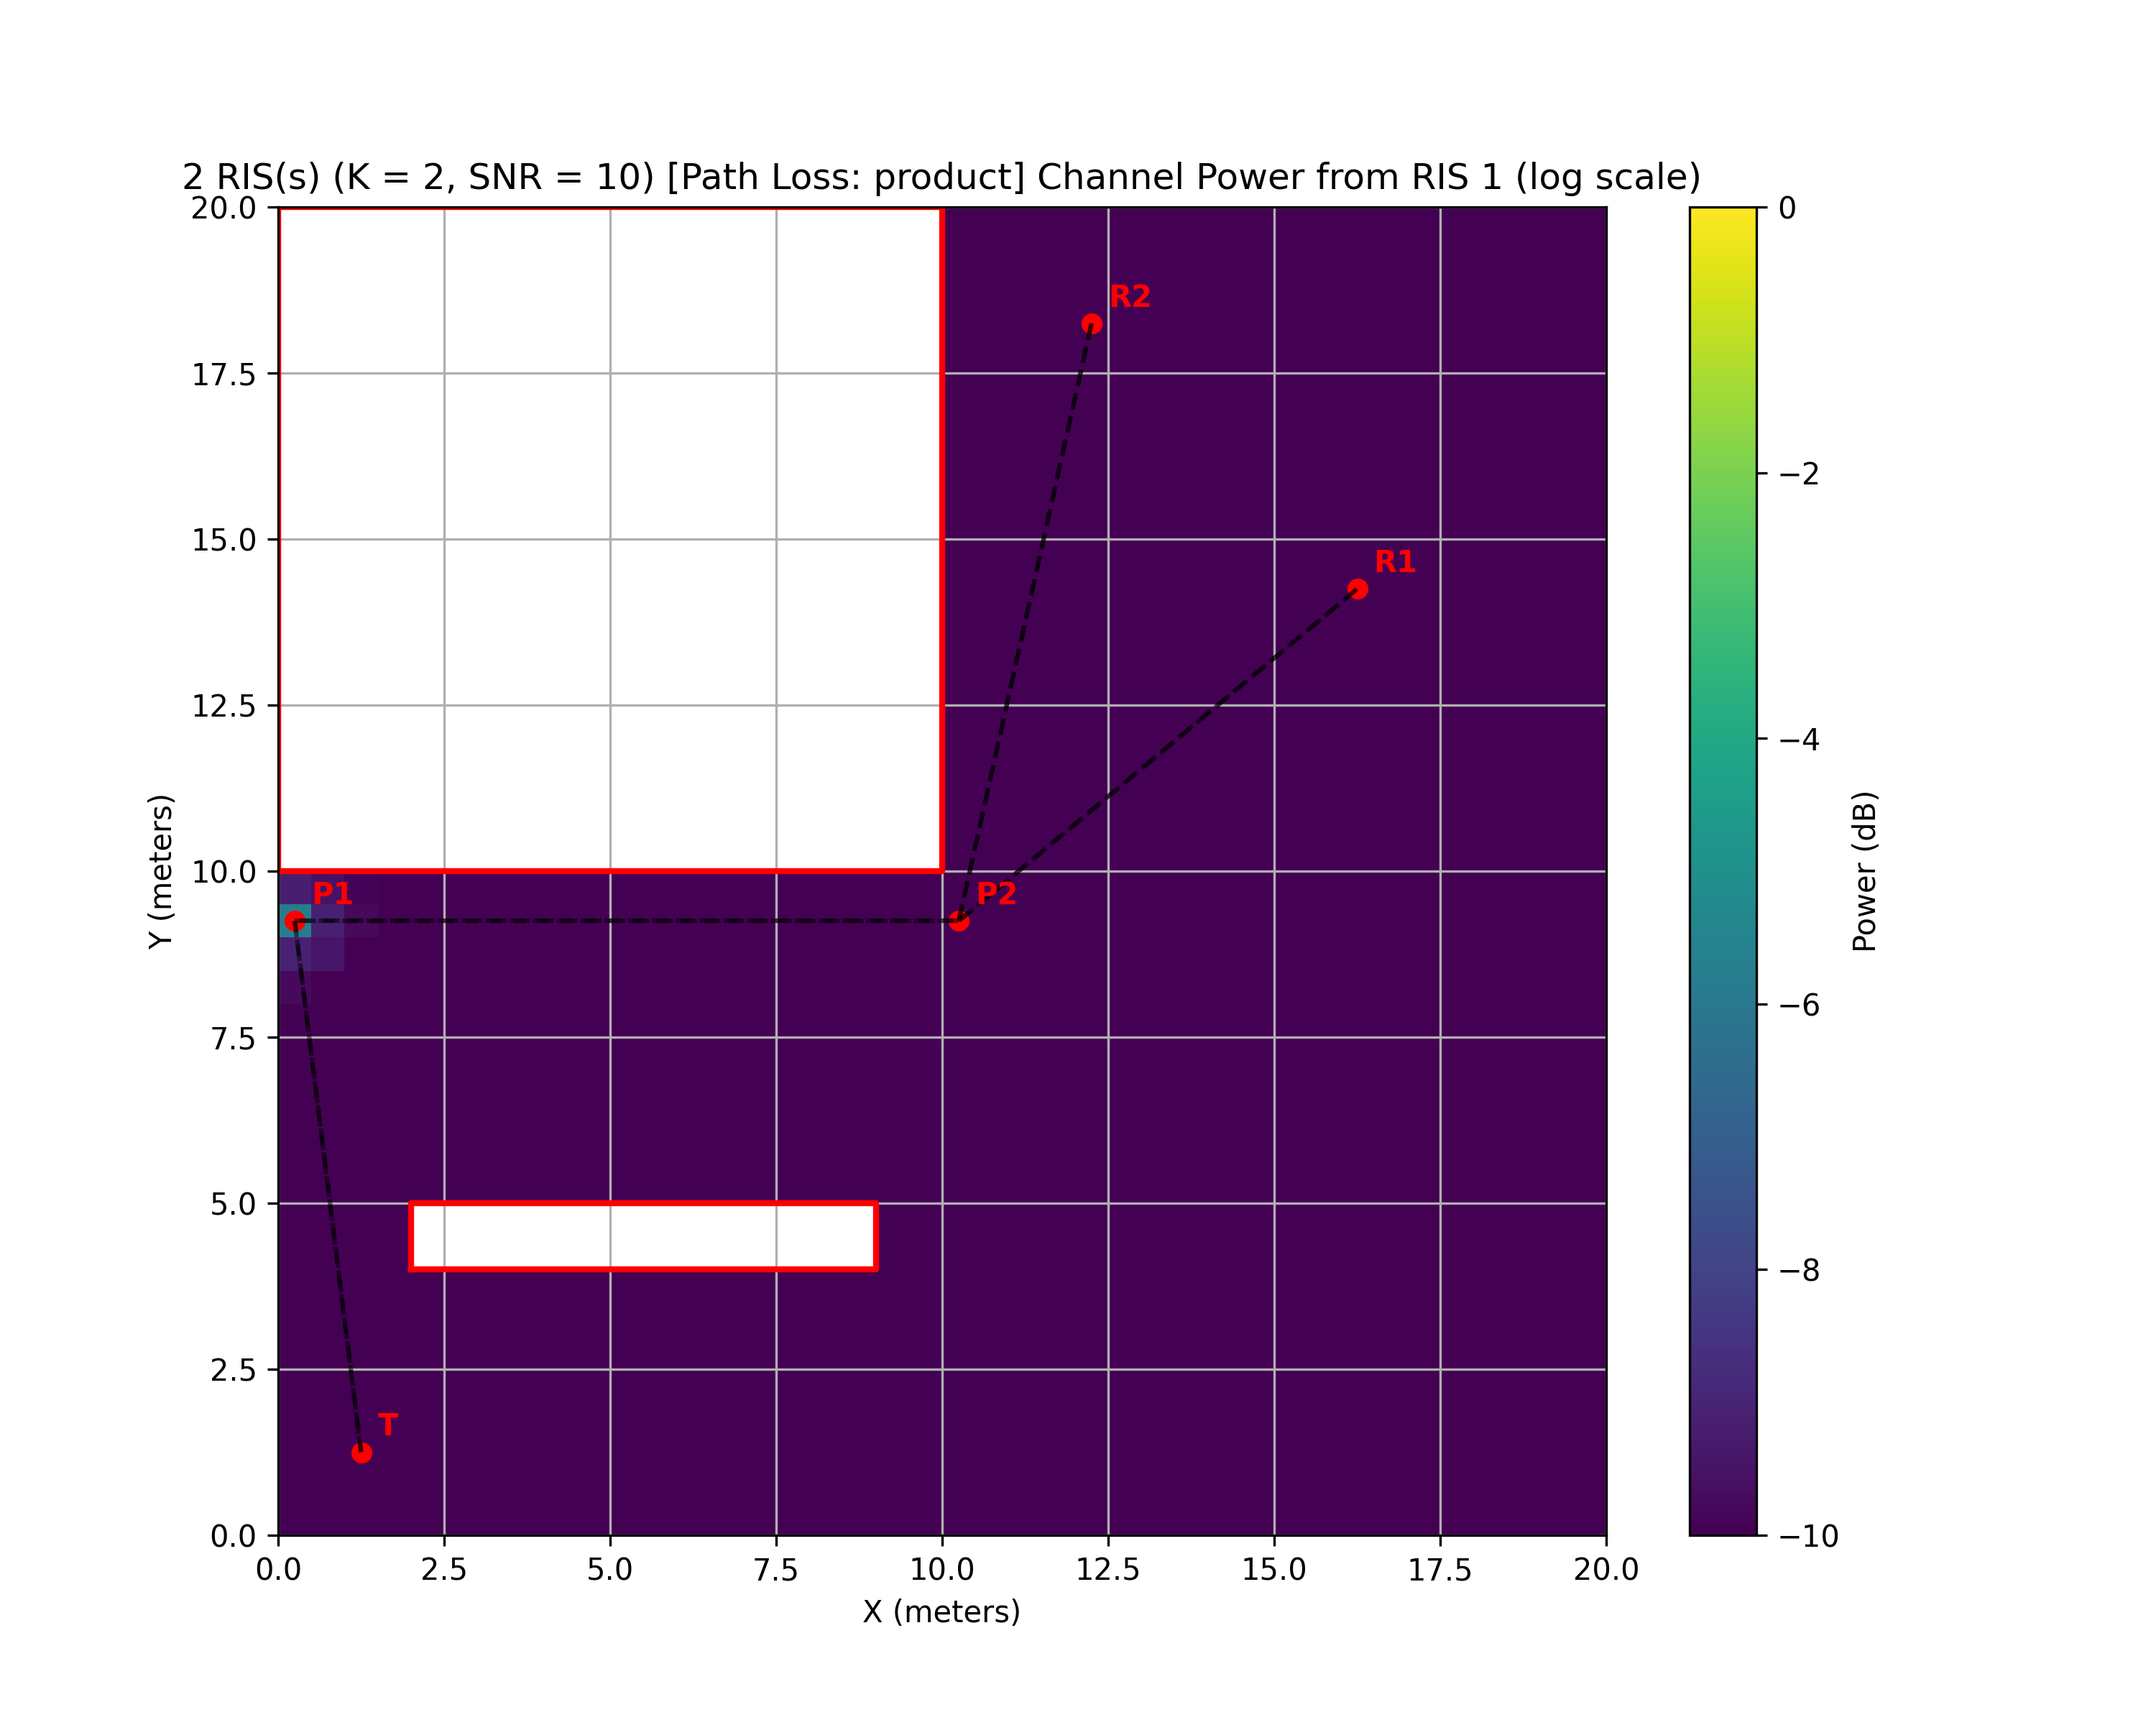
\includegraphics[width=0.7\linewidth]{imgs/heatmap-simulations/2 RIS(s) (K = 2, SNR = 10) [Path Loss_ product] Channel Power from RIS 1 (log scale).png}
  \caption{2 RIS(s) [Path Loss: product] Channel Power from RIS 1 (log scale)}
\end{figure}

\begin{figure}[H]
  \centering
  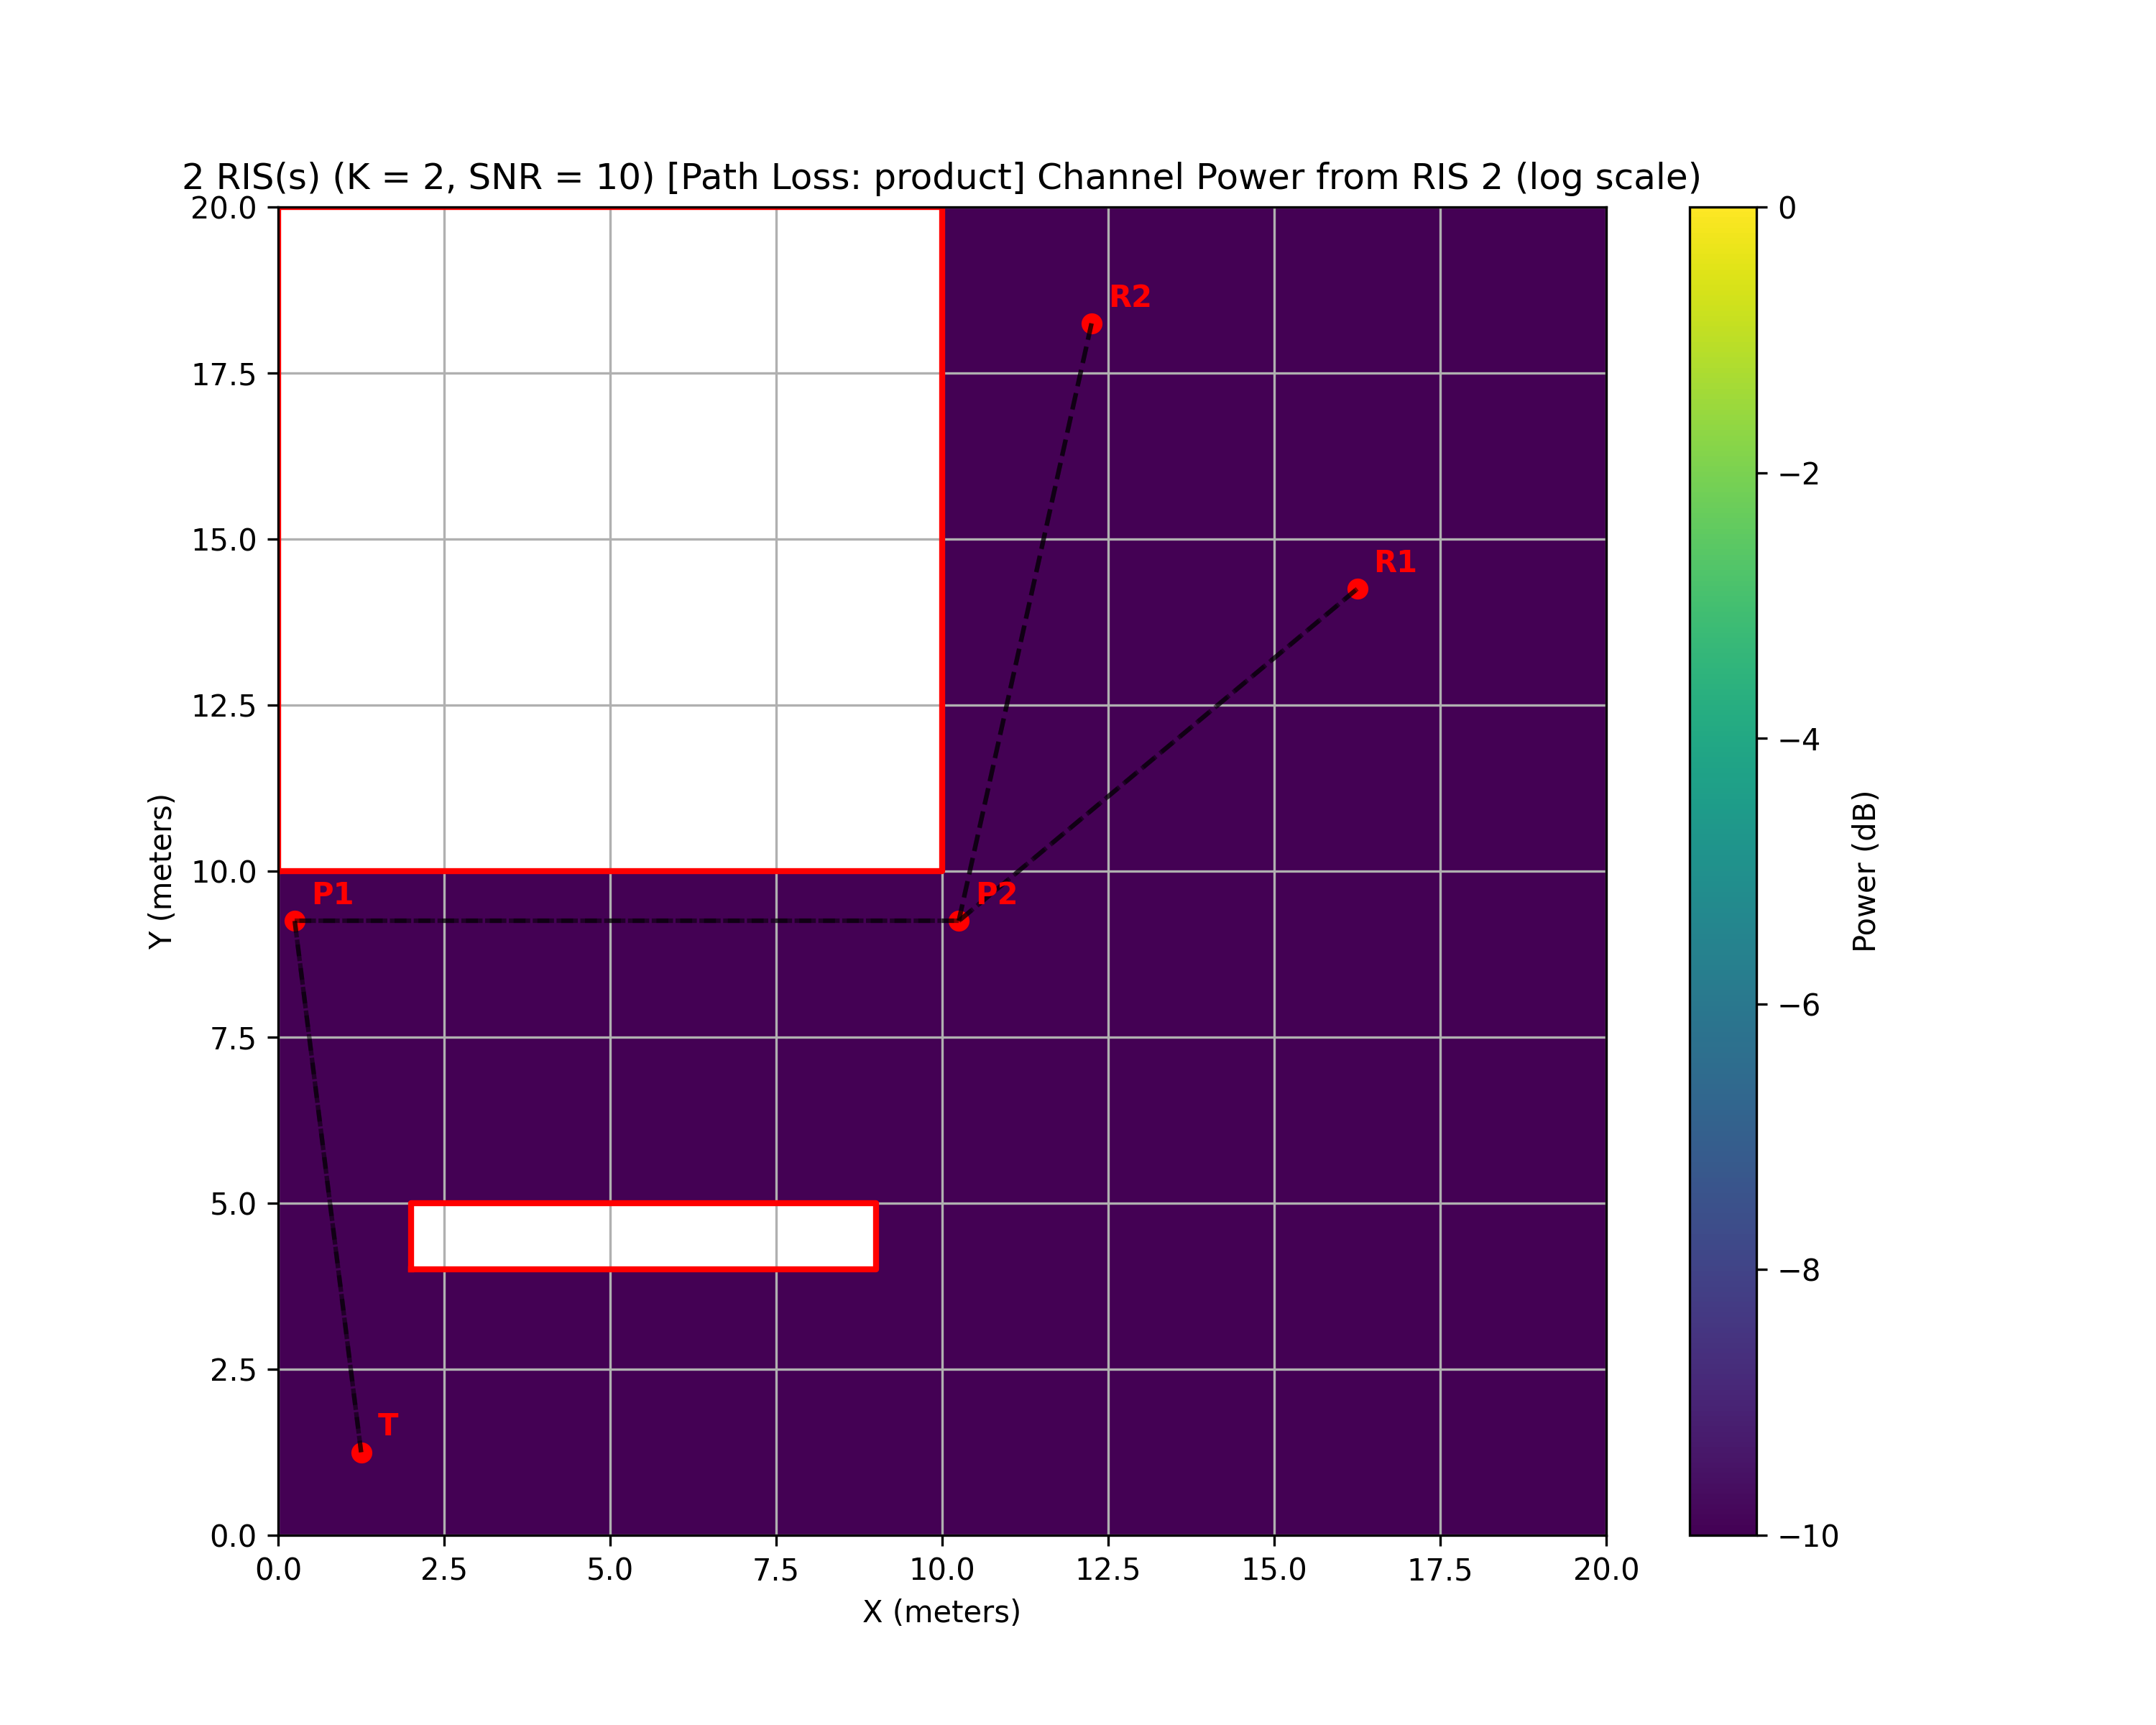
\includegraphics[width=0.7\linewidth]{imgs/heatmap-simulations/2 RIS(s) (K = 2, SNR = 10) [Path Loss_ product] Channel Power from RIS 2 (log scale).png}
  \caption{2 RIS(s) [Path Loss: product] Channel Power from RIS 2 (log scale)}
\end{figure}

\begin{figure}[H]
  \centering
  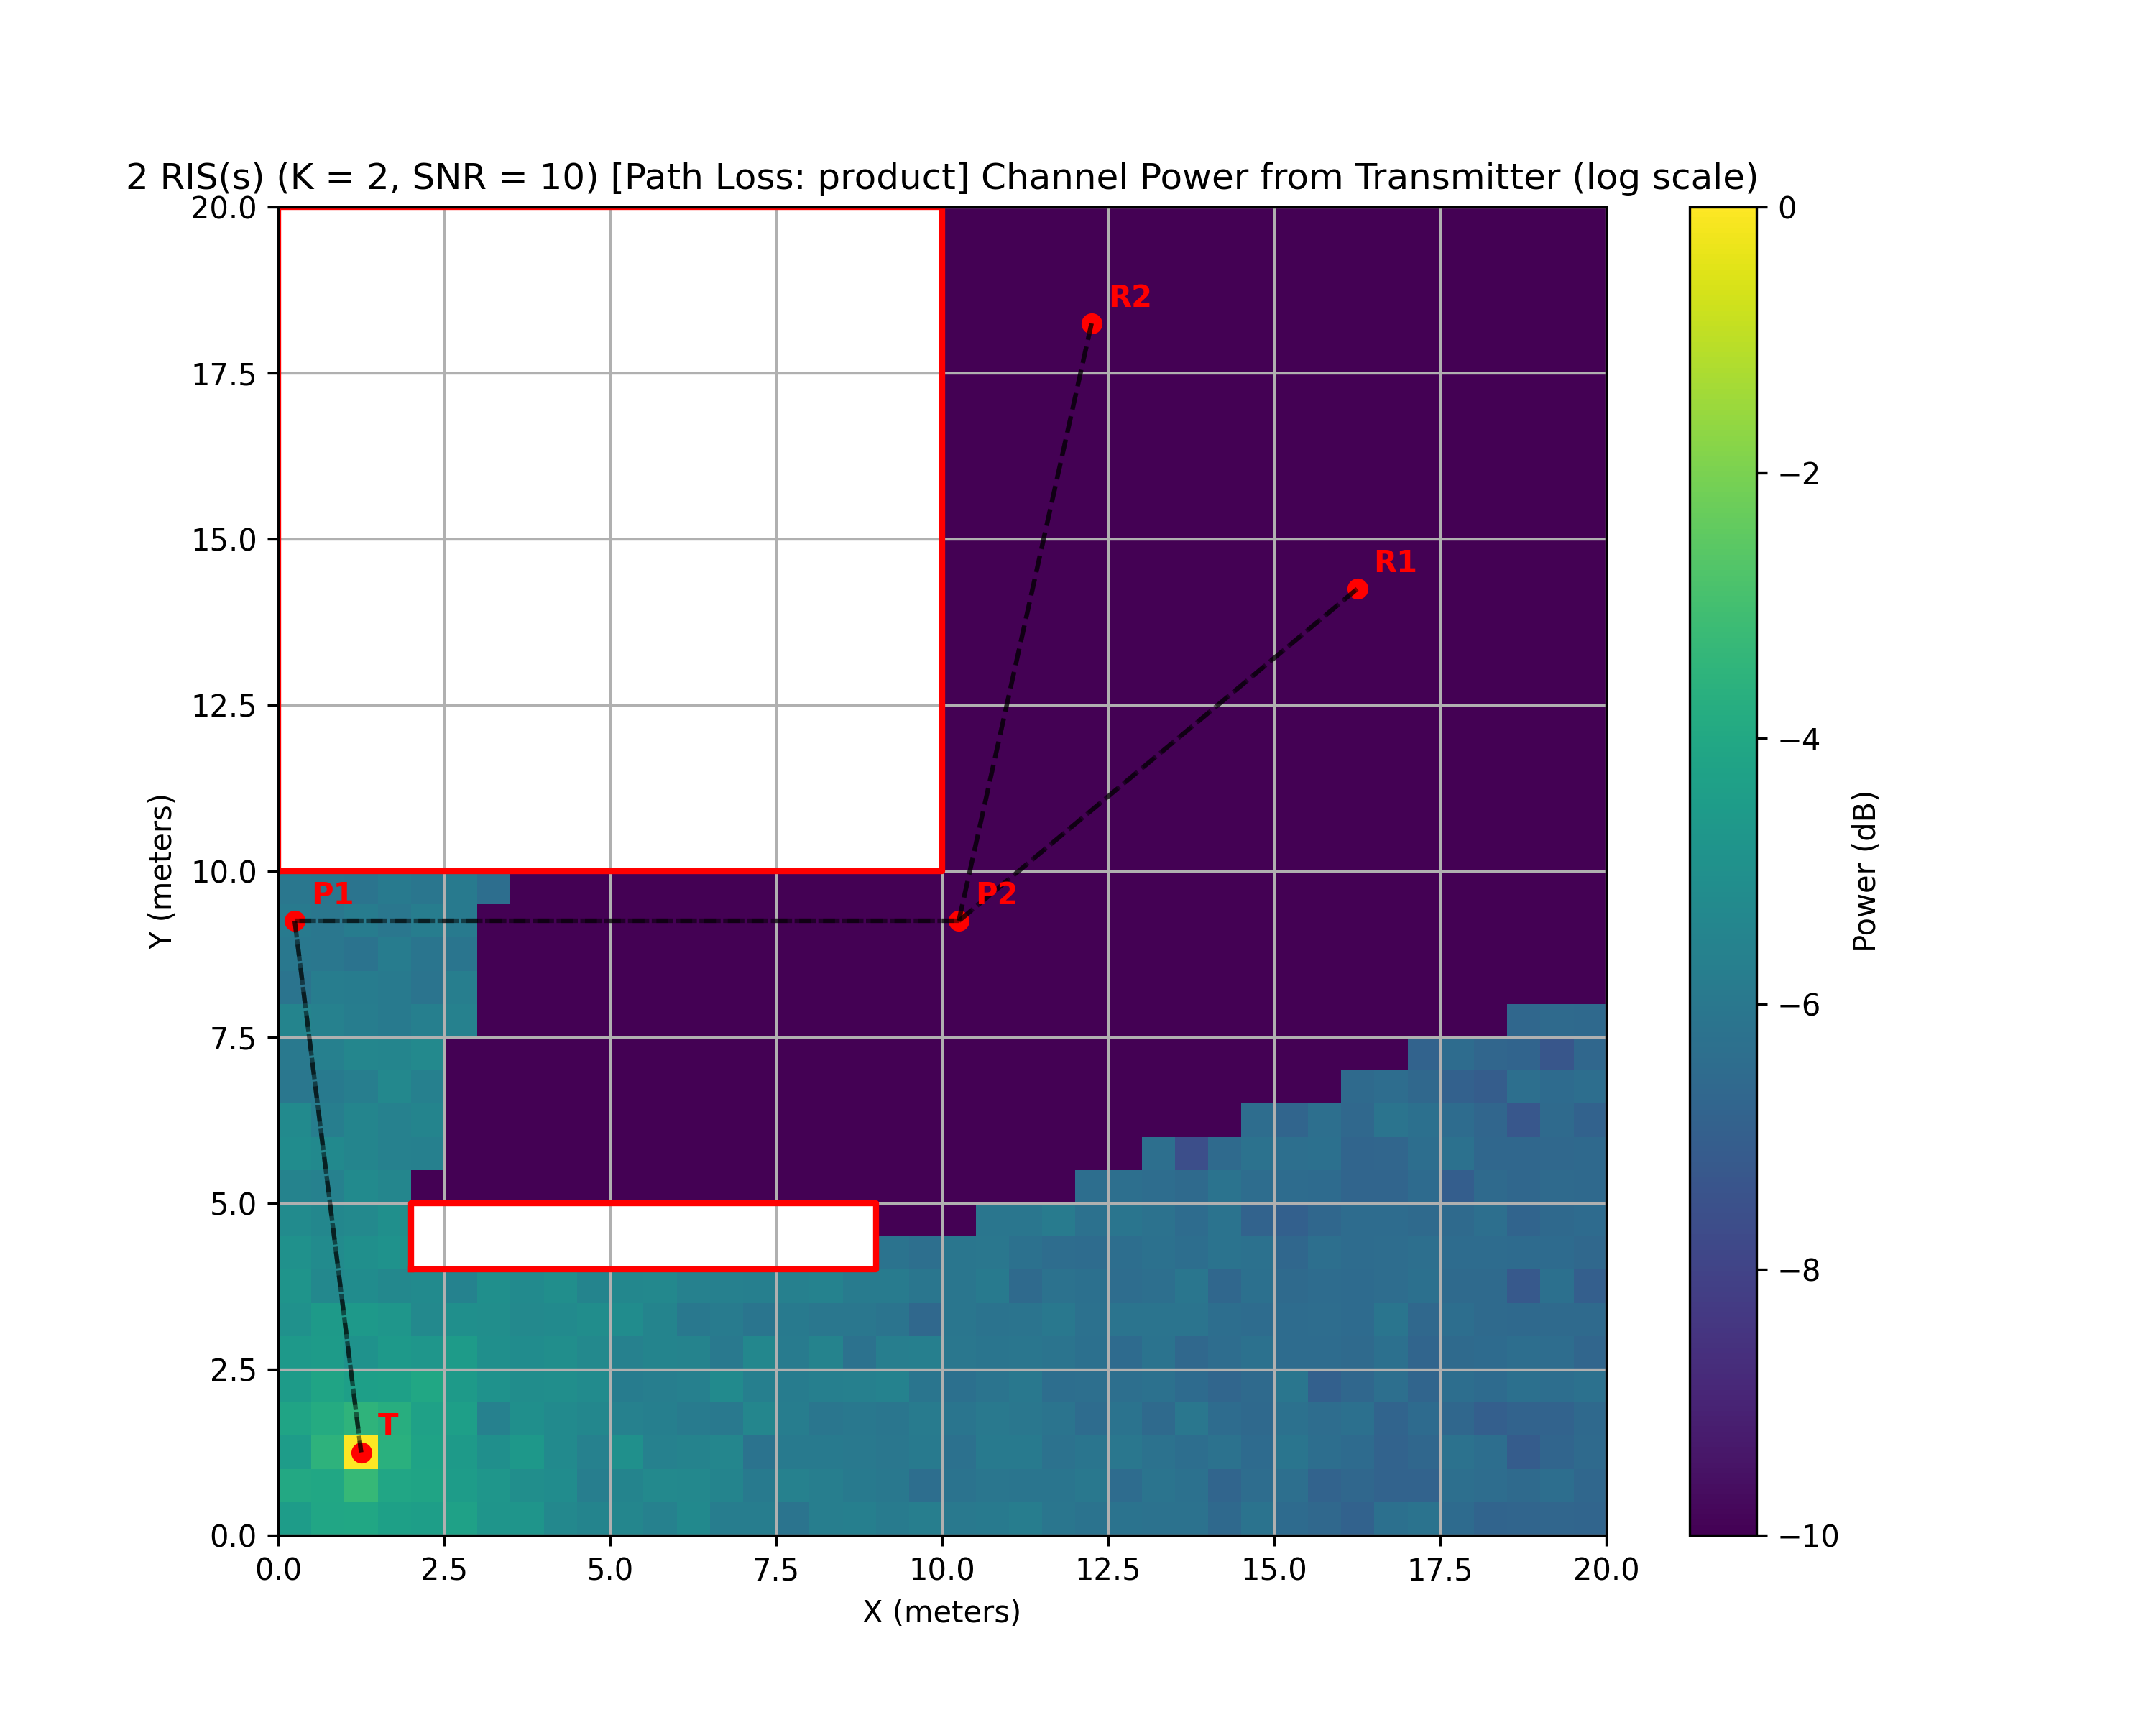
\includegraphics[width=0.7\linewidth]{imgs/heatmap-simulations/2 RIS(s) (K = 2, SNR = 10) [Path Loss_ product] Channel Power from Transmitter (log scale).png}
  \caption{2 RIS(s) [Path Loss: product] Channel Power from Transmitter (log scale)}
\end{figure}

\paragraph*{Path loss: sum}
The distinction between having or not LOS are very visible here. The displayed values for the BER are in line with the previous graph on the same kind of path loss.

Like the active path loss, here there is no difference in having a single disturbance from \textbf{P2} versus from both \textbf{P1} and \textbf{P2}.

We do remember also here that this graph is not realistic, as RIS should be directional. Again, we invite you to consider this as the sum of all possible direction the RIS could take.

\begin{figure}[H]
  \centering
  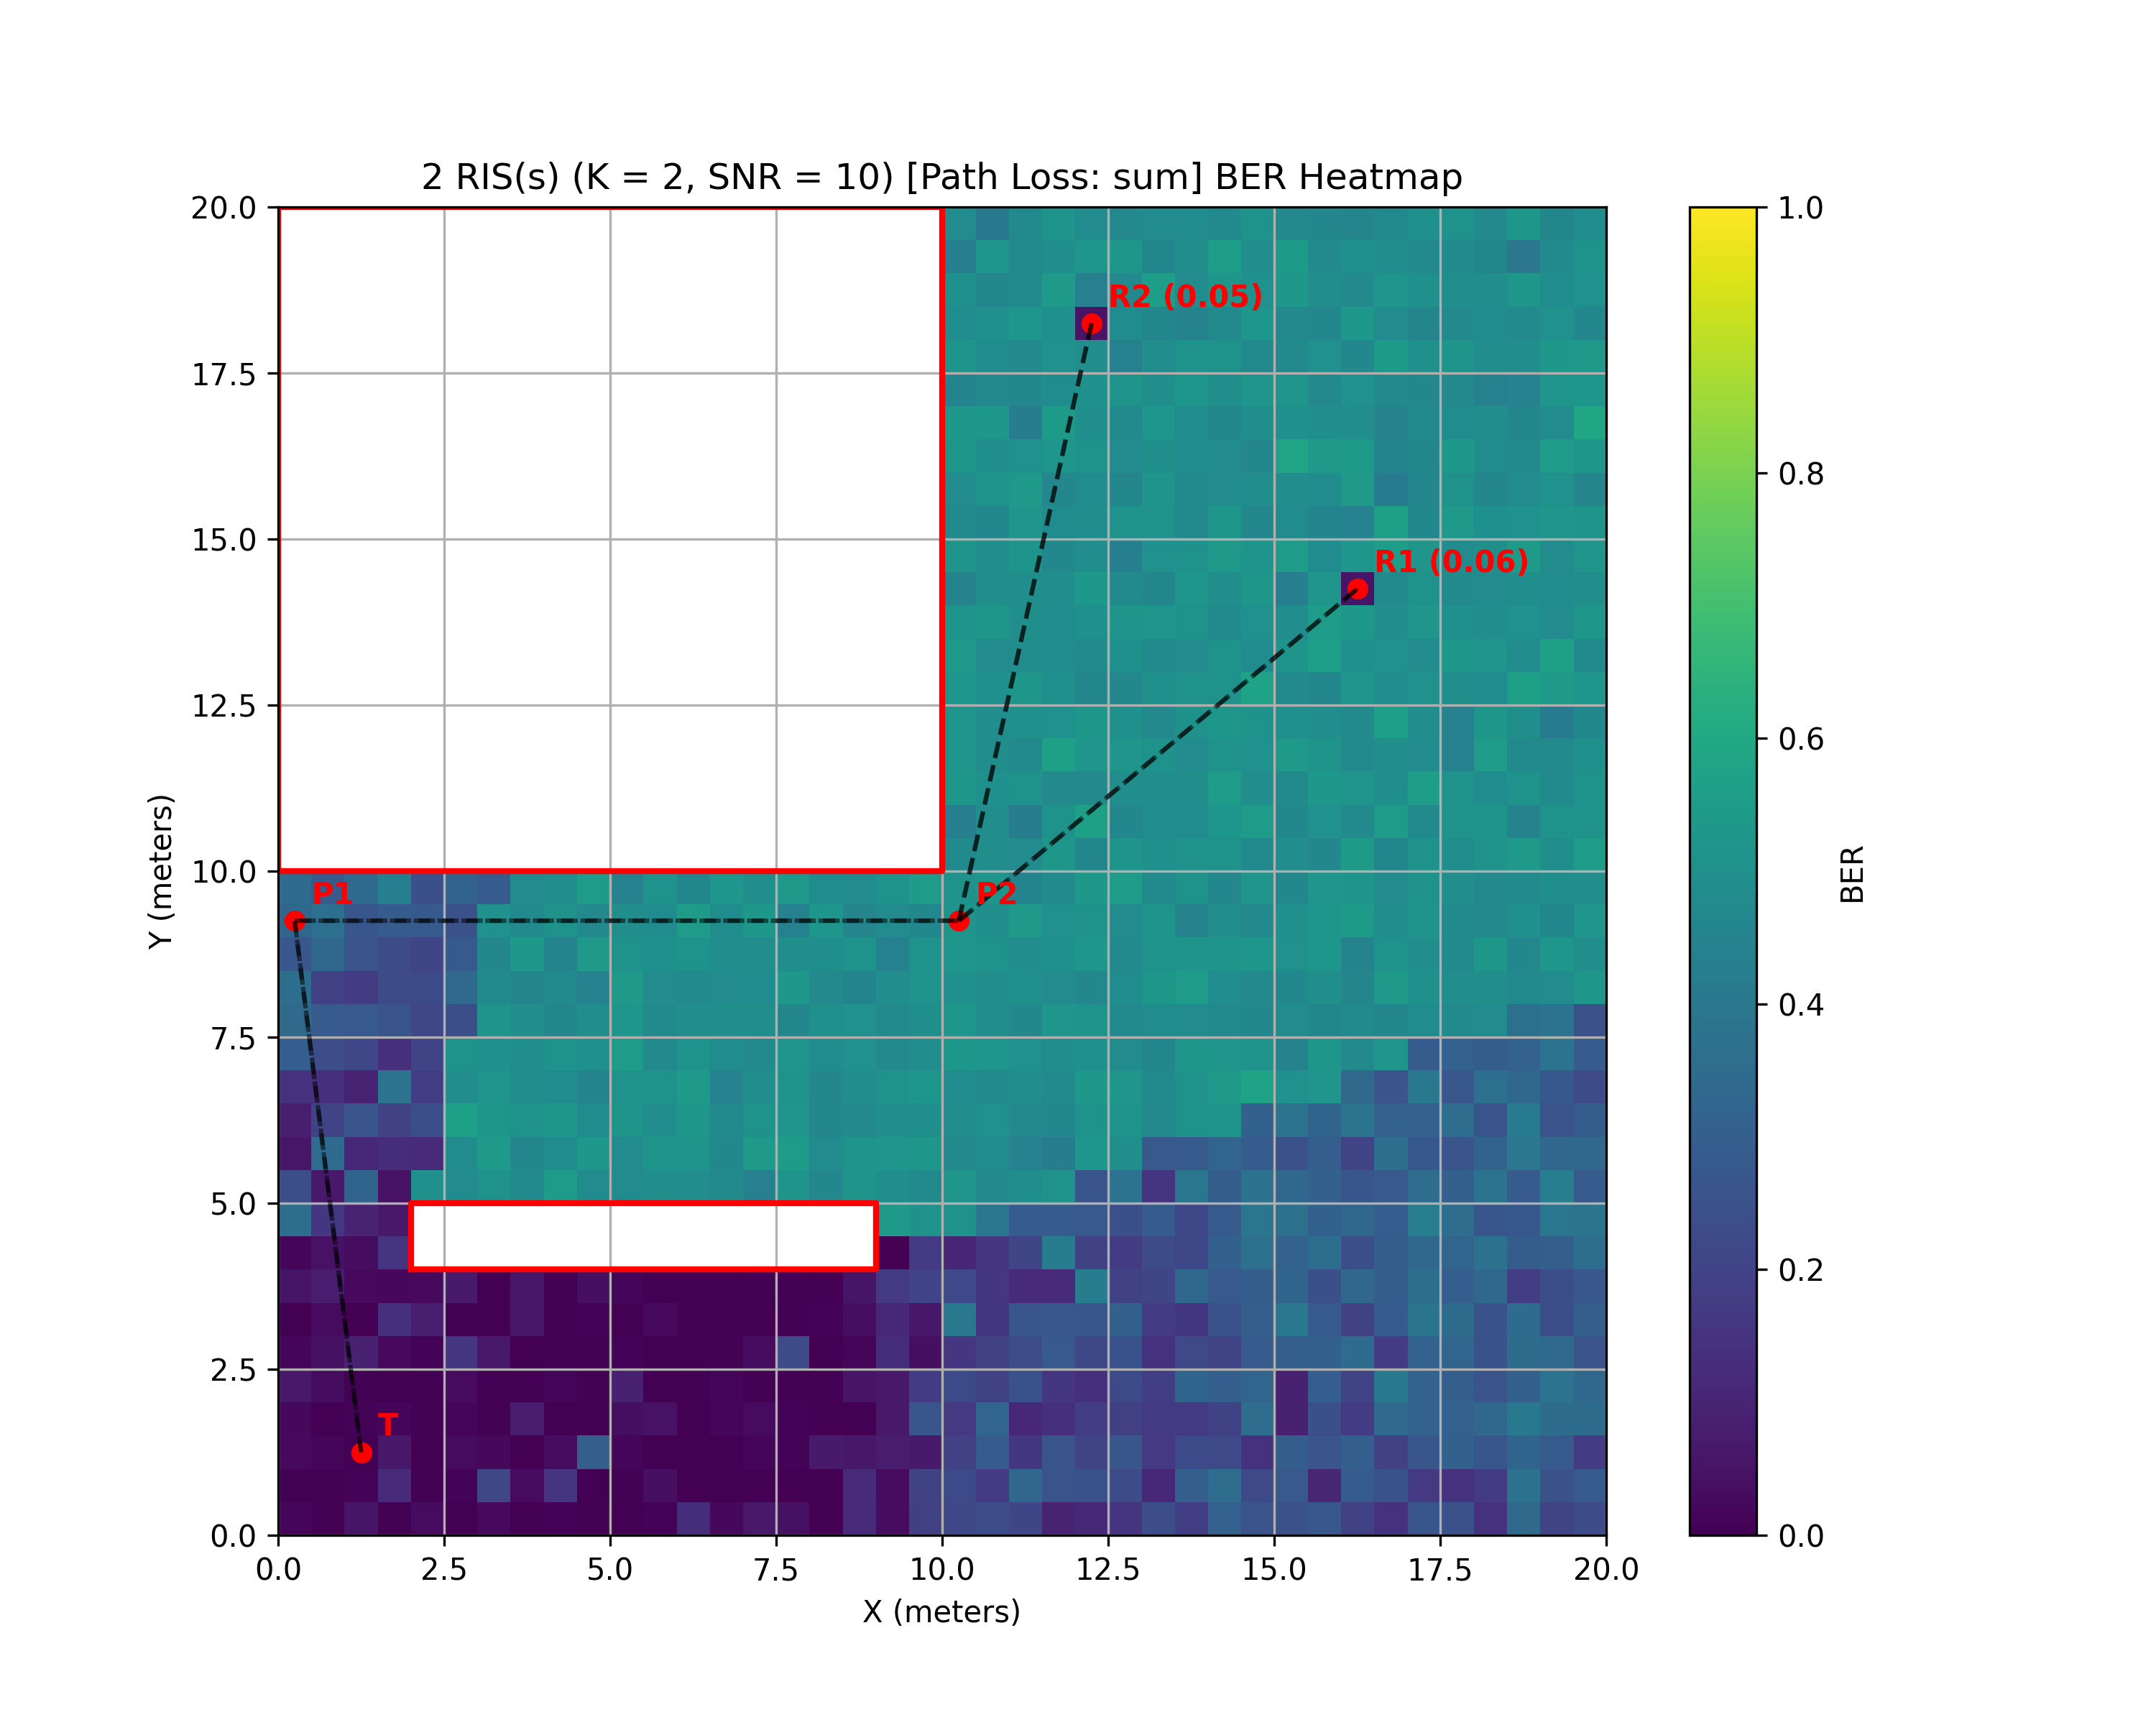
\includegraphics[width=0.7\linewidth]{imgs/heatmap-simulations/2 RIS(s) (K = 2, SNR = 10) [Path Loss_ sum] BER Heatmap.png}
  \caption{2 RIS(s) [Path Loss: sum] BER Heatmap}
\end{figure}

\begin{figure}[H]
  \centering
  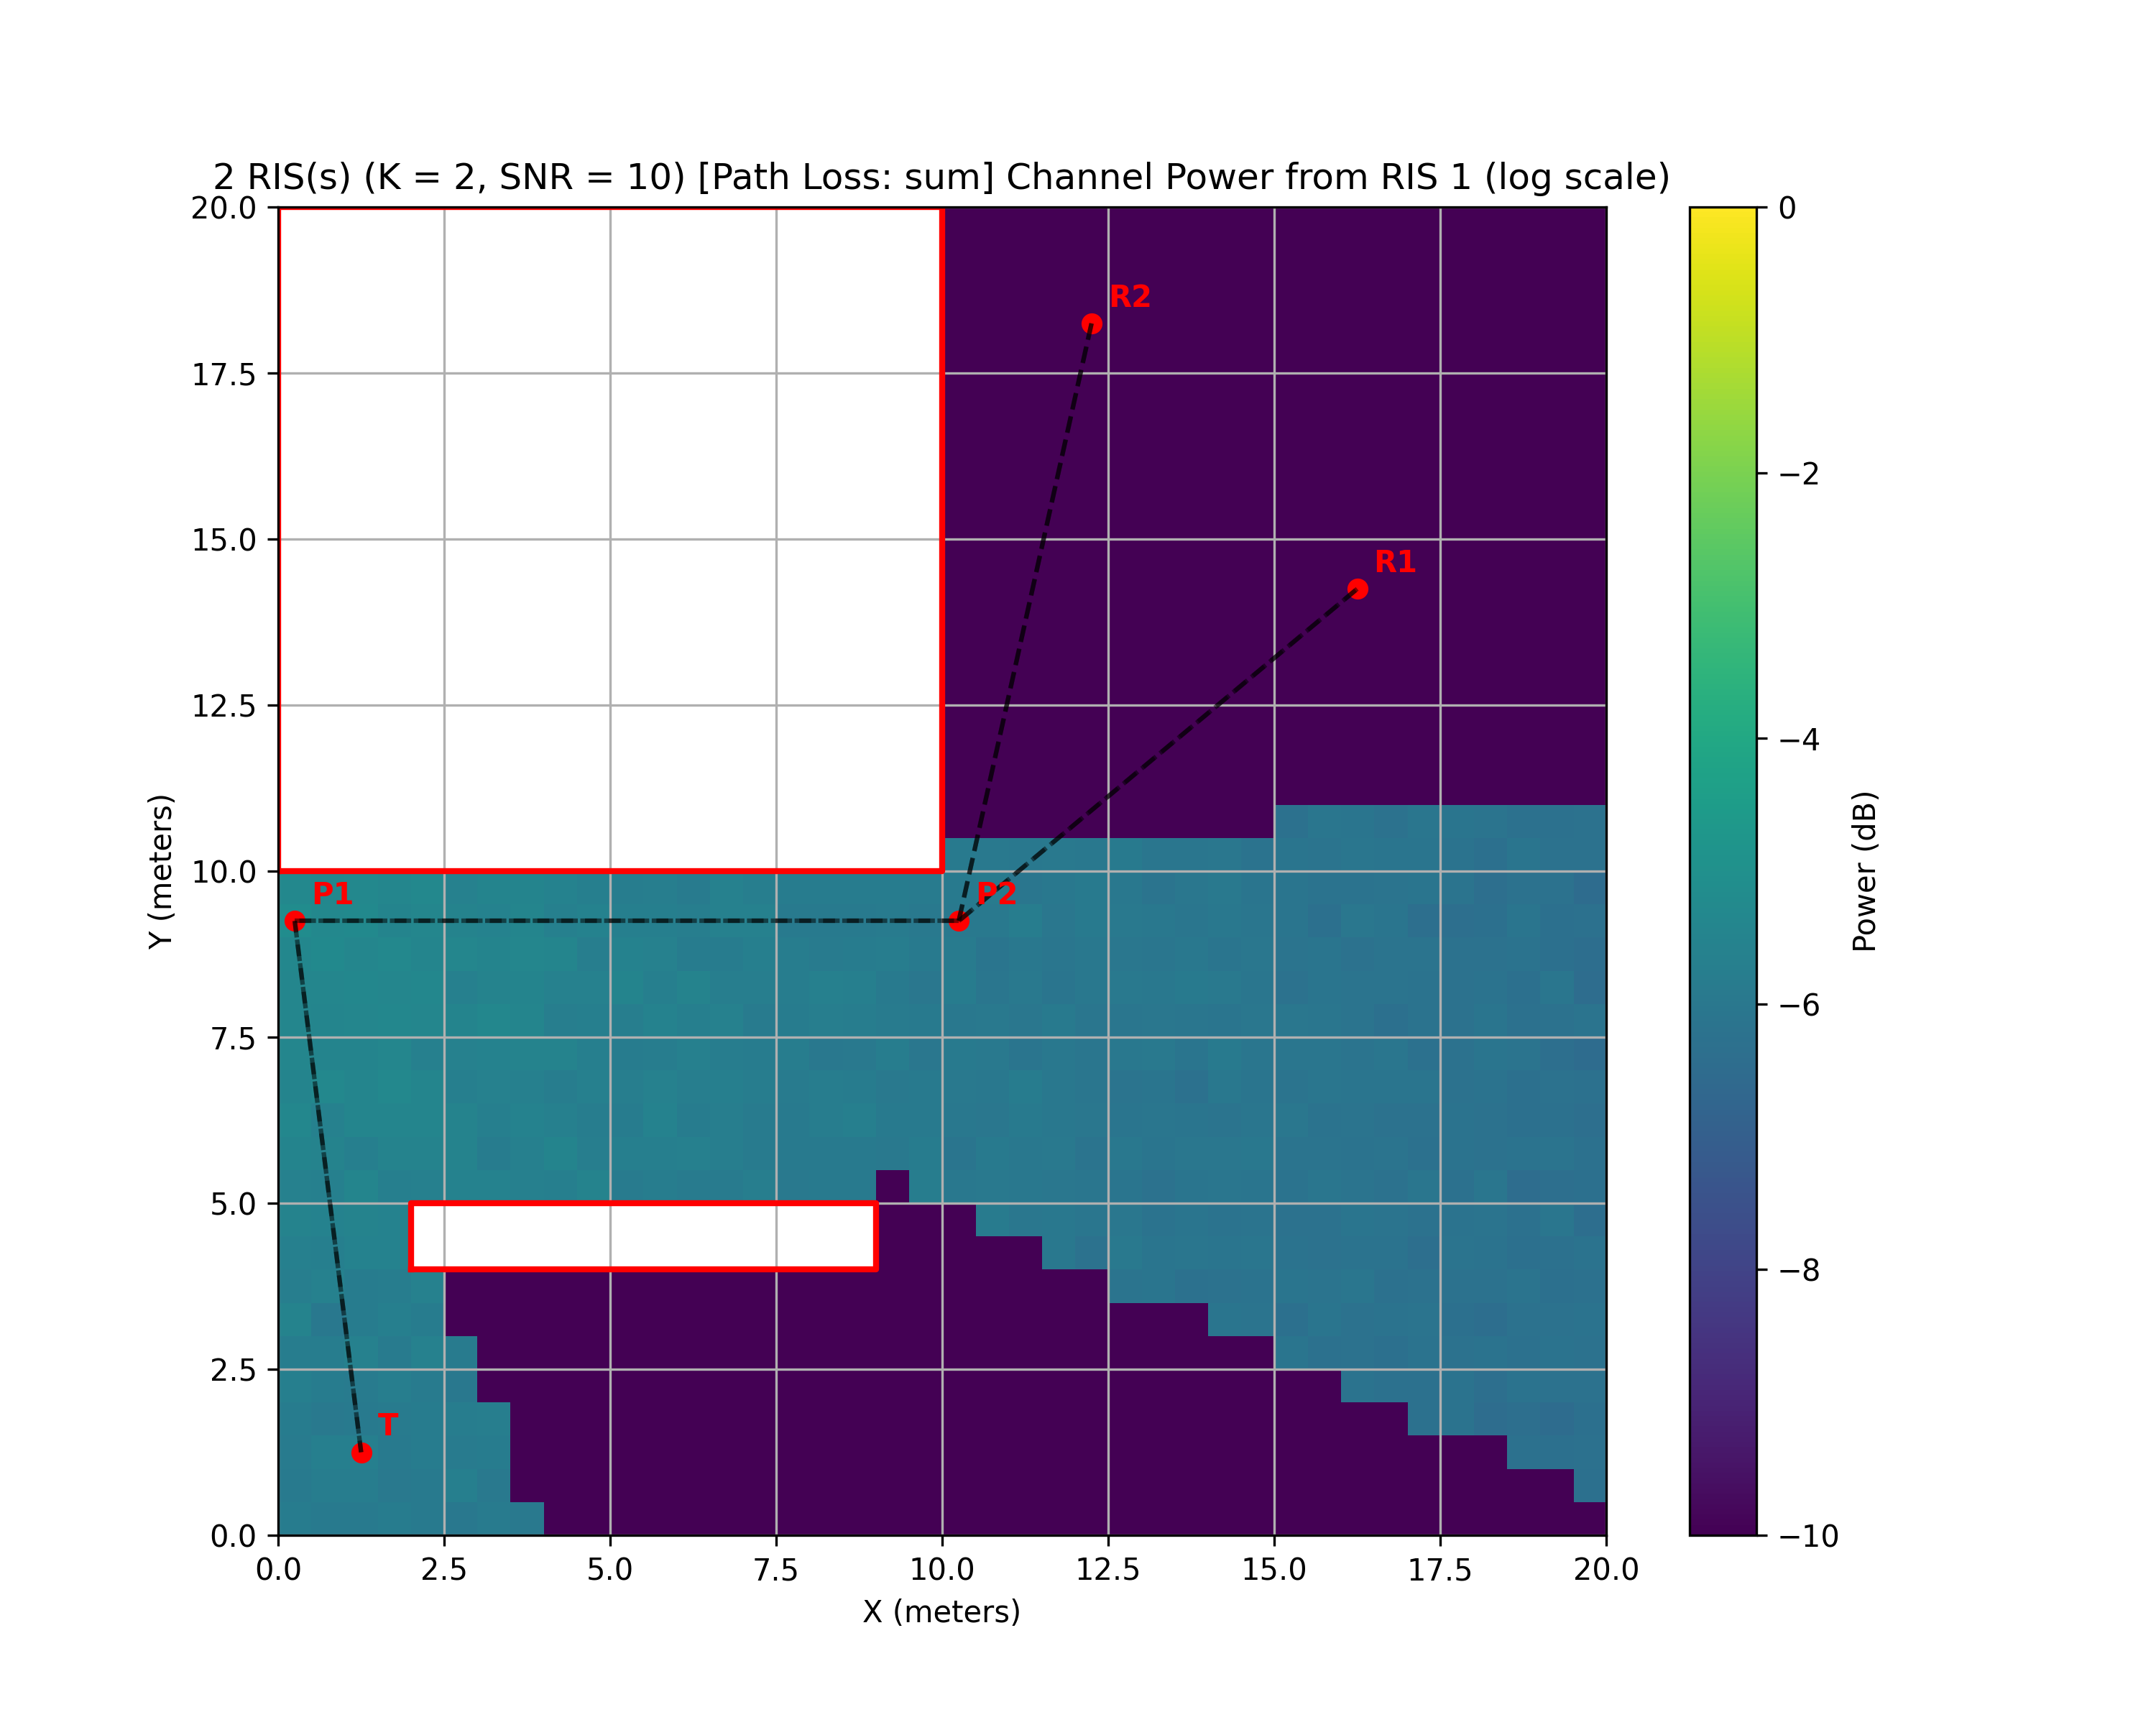
\includegraphics[width=0.7\linewidth]{imgs/heatmap-simulations/2 RIS(s) (K = 2, SNR = 10) [Path Loss_ sum] Channel Power from RIS 1 (log scale).png}
  \caption{2 RIS(s) [Path Loss: sum] Channel Power from RIS 1 (log scale)}
\end{figure}

\begin{figure}[H]
  \centering
  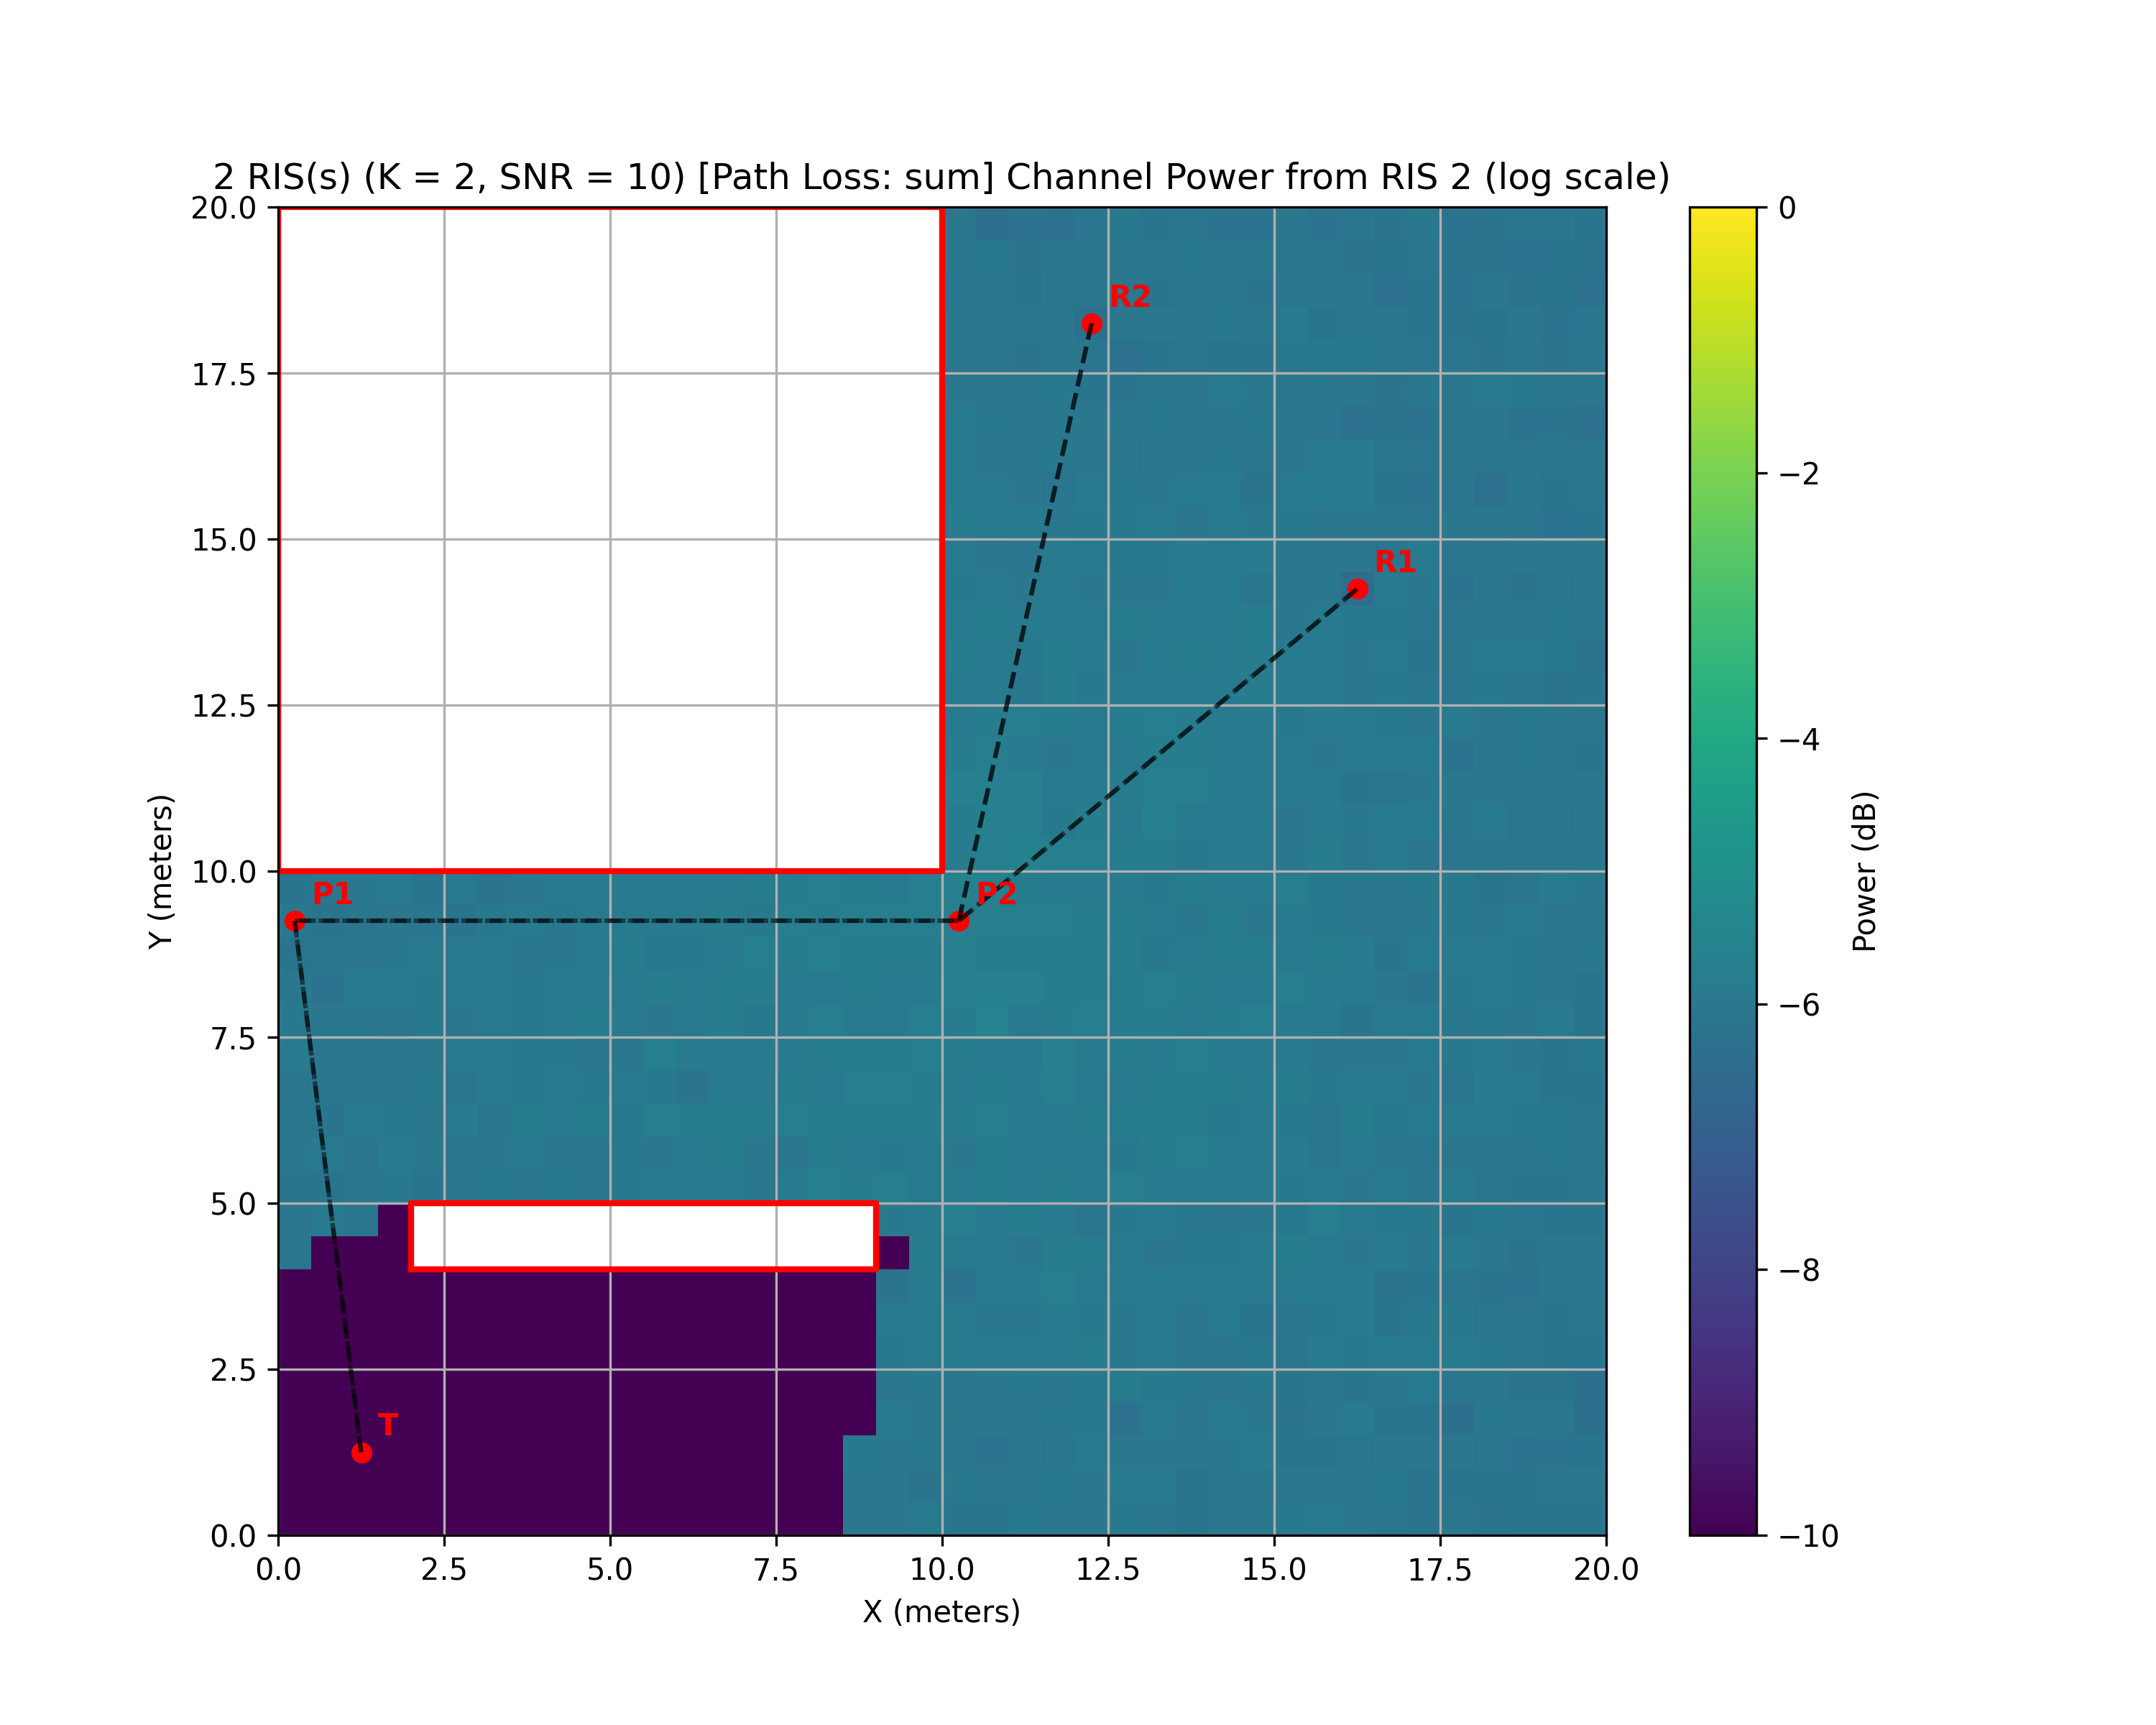
\includegraphics[width=0.7\linewidth]{imgs/heatmap-simulations/2 RIS(s) (K = 2, SNR = 10) [Path Loss_ sum] Channel Power from RIS 2 (log scale).png}
  \caption{2 RIS(s) [Path Loss: sum] Channel Power from RIS 2 (log scale)}
\end{figure}

\begin{figure}[H]
  \centering
  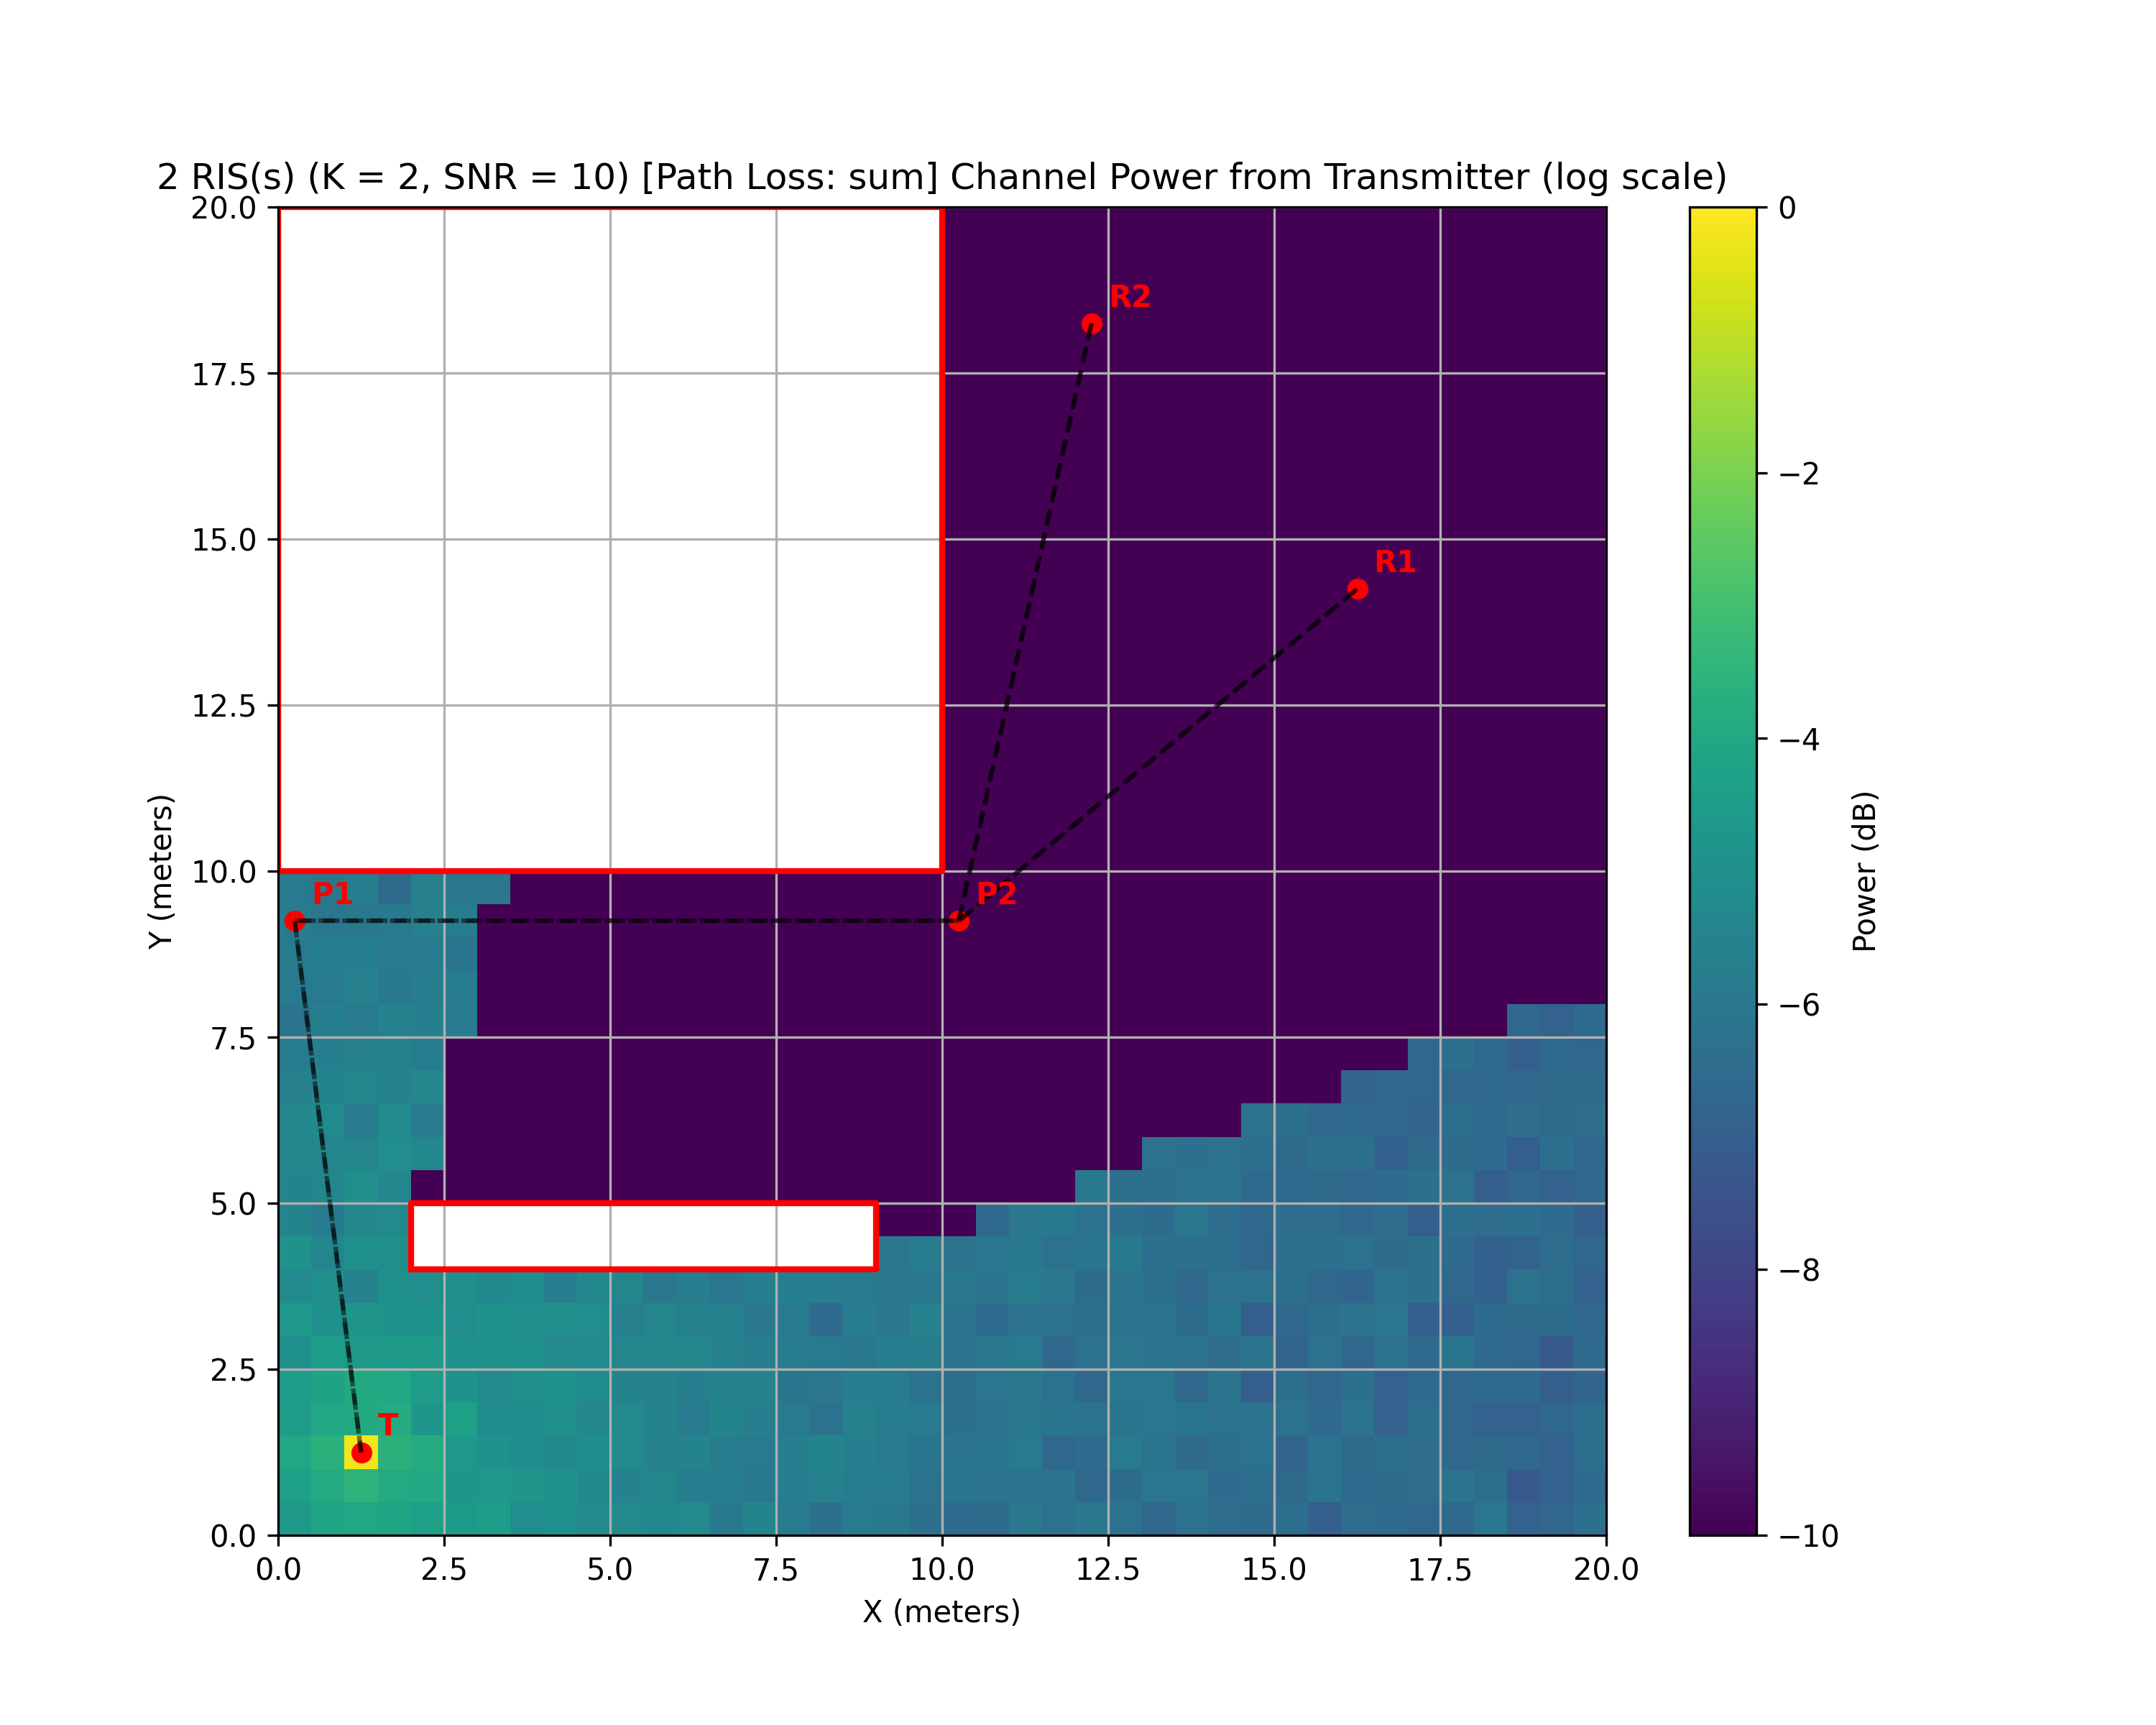
\includegraphics[width=0.7\linewidth]{imgs/heatmap-simulations/2 RIS(s) (K = 2, SNR = 10) [Path Loss_ sum] Channel Power from Transmitter (log scale).png}
  \caption{2 RIS(s) [Path Loss: sum] Channel Power from Transmitter (log scale)}
\end{figure}

\subsubsection{Heatmap conclusions}

We can see from the proposed path loss common properties:

\begin{itemize}
  \item with \textit{active path loss}, the RIS channel power is of the same order of magnitude as the transmitter channel power, so the direct signal receives significant noise. The problem is that, being an active RIS, it costs way more in both the deployment and the maintenance;
  \item with \textit{product path loss}, the RIS channel power is orders of magnitude smaller. The message remains hidden in areas without direct line of sight to the transmitter. If the budget is tight, or the direct LOS security is less needed compared to the non LOS security (for example, if the space in LOS with the transmitter is completely under control), this is an excellent possibility;
  \item with \textit{sum path loss}, the disturbance effect is still visible, although less effective. It also the one with the results most similar to the theoretical simulation we made in the previous section. Of course, the results must be considered keeping in mind that the RIS would be directional. It is an optimal choice for example to provide noise in a specific area, or if the scenario is composed of tight hallways.
\end{itemize}

Depending on the scenario, the budget and the level of security and obscuration needed, our framework provides an excellent choice for different kinds of situations and contexts.

Unfortunately, for specific vehicular applications, our framework is not really flexible due to the specific relation between the position, the distance and the channel gain matrix which then influence the readability of the signal. Our framework is still usable and highly recommended for static antennas and actors. For example, in a crossroad fixed antennas could communicate with the cars in the LOS using standard communication protocols, and with each other using RIS and our framework. The autonomous cars could also implement a traffic light - free crossroad queue system, when they would stop, communicate and coordinate with each other for who can go first. Common distributed algorithms for leader election could be used, like the \textit{Bully Algorithm} \cite{Bully_algorithm}.

It should be noted that the main difficulty in using our framework in conjunction with high speed moving vehicles is because of the channel gain estimation, since we do not only need the current one, but predict the next one where the car would go. Promising results are already coming in like in the paper "\textit{Adaptive Massive MIMO for fast moving connected vehicles: It will work with Predictor Antennas!}" \cite{8385489}, which studies how to use a different set of antennas, called Predictor Antennas, used to predict the main one channel gain with great accuracy. Similar literature can be found, showing a great interest in the field. For example, we also cite "\textit{Channel Estimation for Reconfigurable Intelligent Surface Assisted High-Mobility Wireless Systems}" \cite{9875062}, which proposes a new way to mitigate the error deriving from the movement speed, \textit{achieving substantial power efficiency improvements} at speeds up to 90 mph and with as few as $N=16$ RIS elements.